\chapter{Run II preparation}
\label{CHAPTER:RunIIPreparation}

% \glsresetall % Resetting all acronyms

%Status: DONE (reviewed J.Pela x1) 23Feb - LightTreeAna/test/LTAnalysis (plots) -> plotter
% indico 

After the successful completion of the first data taking period, the  Run I of the \gls{LHC}, the accelerator and detectors went through a two year long technical shut-down which was designated the \gls{LS1}. During this period the accelerator completed a consolidation and improvement program to allow a ramp up of the beams energy up to the design value of $7\,\TeV$ per beam in proton-proton mode. At the same time the experiments also performed maintenance, repair and improvement programs. 

Data analysis continued during this period of no data taking using the datasets already available or the newly reconstructed parked data. Gradually \gls{CMS} physics analysis groups started finishing their Run I analyses and shifted their focus to the preparation for the Run II of the \gls{LHC}, where higher collision energies, higher values of \gls{PU} and more recorded integrated luminosity are expected. As part of this global effort, the \gls{CMS} \gls{VBF} Higgs to invisible analysis also started its own preparation work. 

The first step is always the definition of a trigger condition for data taking. The effort made to define and study an adequate set of triggers is documented in section \ref{SECTION:RunIITriggerStudies}. Additionally, a study was conducted that led to the proposal of the creation of a dedicated \gls{QCD} \gls{MC} sample with signal-like characteristics expanding on similar samples made for Run I. This study can be found in section \ref{SECTION:RunIIPreparation_RunIIQCDMonteCarloSamples}.

%%%%%%%%%%%%%%%%%%%%%%%%%%%%%%%%%%%%%%%%%%%%%%%%%%%%%%%%%%%%%%%%%%%%%%%%%%%%%%%%%%%%%%%
%%% SECTION
%%%%%%%%%%%%%%%%%%%%%%%%%%%%%%%%%%%%%%%%%%%%%%%%%%%%%%%%%%%%%%%%%%%%%%%%%%%%%%%%%%%%%%%
\section{Run II trigger studies}
\label{SECTION:RunIITriggerStudies}

% Working areas
% 
% /vols/cms02/jca10/work/slc6/dev01/CMSSW_7_2_0_pre8/src
% /vols/cms02/jca10/work/slc6/dev01/testPhD/CMSSW_7_2_0_pre8/src
%
% Executable:
% /vols/cms02/jca10/work/slc6/dev01/testPhD/HEPFW/src/VBFHiggsToInvisible/TriggerAnalysisRun2015/exe/vbfinv_getTriggerResults.cxx
%
% L1T plots
% cd /vols/cms02/jca10/work/slc6/dev01/testPhD/CMSSW_7_2_0_pre8/src/jobs
% vbfinv_getTriggerResults --l1t
% cd /vols/cms02/jca10/work/slc6/dev01/testPhD/CMSSW_7_2_0_pre8/src/jobs/Run_1/SameDijet/DijetVBF30_DEta3p5/ <- Plots here
%
% HLT plots
% cd 
% vbfinv_getTriggerResults --hlt2 HLT_Run2015_ETM70/ HLT_Run2015_ETM70_NOTPFMET170/
% vbfinv_getTriggerResults --hlt2 HLT_Run2015_DijetVBF-SingleJet96/ HLT_Run2015_DijetVBF-SingleJet96_NOTPFMET170/
% vbfinv_getTriggerResults --hlt2 HLT_Run2015_DijetVBF-ETM50/ HLT_Run2015_DijetVBF-ETM50_NOTPFMET170/ 
% cd 
%
% Oct 21  2014 jobs
% Oct 14  2014 jobsHLT
% Oct 22  2014 jobsHLTv2
% Oct 22  2014 jobsL1Tv2

% Oct 26  2014 VBFHiggsToInvisible/TriggerStudies/HLT_Run2015
% Oct 26  2014 VBFHiggsToInvisible/TriggerStudies/HLT_Run2015_DijetVBF-ETM50_NOTPFMET170
% Oct 27  2014 VBFHiggsToInvisible/TriggerStudies/HLT_Run2015_ETM70
% Oct 27  2014 VBFHiggsToInvisible/TriggerStudies/HLT_Run2015_ETM70_NOTPFMET170
% Oct 27  2014 VBFHiggsToInvisible/TriggerStudies/L1TAddRate

% Additional rates study: 
% /vols/cms02/jca10/work/slc6/dev01/CMSSW_7_2_0/src/VBFHiggsToInvisible/

%Status: DONE (reviewed J.Pela x1)

The first step of any \gls{CMS} physics analysis is to define which trigger to use for data taking. The \gls{TSG} develops generic usage trigger conditions, know as trigger paths, which can be used by any analysis. Typically these conditions cover all possible single objects (single electron, single jets, etc), multiple objects (double electron, triple muon, etc), cross triggers (single electron $+$ sigle muon, etc) and sums (\gls{MET}, \gls{HT}, etc). In some cases, as for this analysis, it is better to define a custom condition to obtain maximum physics content at trigger level. The following reasons drove the decision to create a set of dedicated trigger paths.

\begin{itemize}
  \item Maximize signal collection efficiency by selecting our signal topology with reduced trigger thresholds compared to generic triggers;
  \item Use a trigger condition with $\text{MET}_{no-\mu}$ instead of MET to study the irreducible \gls{EWK} Z background;
  \item Create a new dedicated prescaled trigger path with reduced thresholds with objective of reducing systematics;
\end{itemize}

In order to propose new triggers, it was decided to consider low rate and high rate scenarios in terms of the available \gls{L1T} and \gls{HLT} bandwidth. For the \gls{L1T}, the low rate scenario was the usage of only the lowest threshold unprescaled \gls{MET} algorithm on the menu, while for the high rate scenario a dedicated additional \gls{L1T} seed algorithm with a pure rate (without accounting for overlaps with other trigger) of up to $5\,\kilo\hertz$ would be proposed. For the \gls{HLT} signal trigger path, rates of $1.5\,\hertz$ and $5.0\,\hertz$ were considered and of $0.1\,\hertz$ and $0.5\,\hertz$ for the background path.

%%%%%%%%%%%%%%%%%%%%%%%%%%%%%%%%%%%%%%%%%%%%%%%%%%%%%%%%%%%%%%%%%%%%%%%%%%%%%%%%%%%%%%%
%%% SUBSECTION
%%%%%%%%%%%%%%%%%%%%%%%%%%%%%%%%%%%%%%%%%%%%%%%%%%%%%%%%%%%%%%%%%%%%%%%%%%%%%%%%%%%%%%%
\subsection{Methodology}
\label{SECTION:RunIITriggerStudies_Methodology}

%Status: DONE (reviewed J.Pela x1)

To study new \gls{L1T} algorithms for a never before attempted collision energy, \gls{MC} simulation must be used. At this level the system has to analyse all collisions which are produced by the \gls{LHC}, which implies that the test simulated event sample cannot have significant generation cuts. For this purpose, the so called neutrino gun event samples are used. In these event simulations, the hard process is replaced by the production of a single neutrino which will escape the detector without leaving any deposit. \acrfull{PU} events are added to the event following a Poissonian distribution with its centre chosen according to predicted \gls{LHC} performance scenarios. This \gls{PU} events are selected randomly from a large \gls{QCD} multi-jet sample, generated with minimum restrictions. This type of sample normally is denominated by \textit{Minimum Bias \gls{QCD}}. The final event content will be the overlap of many minimum bias events without any hard process as expected from the great majority of collisions.

At the \gls{HLT}, the events are already pre-selected by the \gls{L1T} and the dominating processes at this point are dependent on the characteristics of both the \gls{L1T} seeding algorithm and the \gls{HLT} conditions. For the \gls{CMS} \gls{VBF} Higgs to invisible analysis, the trigger conditions take advantage of the topology of the \gls{VBF} jets and \gls{MET}. These characteristics make high energy \gls{QCD} multi-jet events the dominating source of rate for any \gls{HLT} paths that will collect specifically our signal process.

The trigger system that was present in the beginning of Run II was an upgraded version of the one previously used. As such, its response had to be emulated using available \gls{MC} samples. The latest version available of the \gls{L1T} stage 2 and \gls{HLT} systems description was used to preform these studies.

The target conditions of \gls{LHC} running used in this study and required for the development of new algorithms, the \textit{\gls{TSG} high luminosity scenario}, are an instantaneous luminosity of  $1.4 \times 10^{34}\,\centi\meter^{-2}\second^{-1}$, an average \gls{PU} of 40 collisions and a bunch separation of $25\,\nano\second$. 

%%%%%%%%%%%%%%%%%%%%%%%%%%%%%%%%%%%%%%%%%%%%%%%%%%%%%%%%%%%%%%%%%%%%%%%%%%%%%%%%%%%%%%%
%%% SUBSECTION
%%%%%%%%%%%%%%%%%%%%%%%%%%%%%%%%%%%%%%%%%%%%%%%%%%%%%%%%%%%%%%%%%%%%%%%%%%%%%%%%%%%%%%%
\subsection{L1T algorithm development}
\label{SECTION:RunIITriggerStudies_L1TAlgorithmDevelopment}

%Status: DONE (reviewed J.Pela x1)

In the \gls{L1T} trigger menu, the reference algorithm was selected as the lowest unprescaled \gls{MET} trigger available, which was \verb|L1_ETM70|. This algorithm selects events with \gls{L1T} \gls{MET} of $70\,\GeV$ which is only calculated in $|\eta|<3.0$ range. It has an expected pure rate of $\approx 7\,\kilo\hertz$ and a signal efficiency of 27-28\%. 

When designing an offline analysis, normally it is desirable to select events in a parameter space where the trigger efficiency is close to 100\%, avoiding the need to re-weight the \gls{MC} simulated events to match the trigger behaviour. Unfortunately, even if the default \gls{L1T} algorithm has a reasonable signal collection efficiency, it is likely to only be fully efficient when selecting events with offline \gls{PF} \gls{MET} two to three times higher than the trigger threshold, implying a significant increase of this offline variable requirement when compared with that used during Run I. For these reasons, the priority was to find a solution that would allow a lower threshold to be applied to \gls{L1T} \gls{MET} by requiring additional conditions.

To determine the best possible algorithm, an automatic optimization method was implemented. Several base dijet configurations were defined with one key variable being allowed to float to achieve a target rate. A maximum rate of $5\,\kilo\hertz$ was set as an optimistic acceptable pure rate for such an algorithm. All base configurations start by requiring at least one \gls{L1T} dijet being on opposite sides of the detector (\gls{VBF} condition). Many possible configurations were tested requiring the selected jets to have  $\pt>{30,40}$ and dijet $\Delta\eta>{3.0,3.5}$. Scanned variables included lead jet \pt, sub-lead jet \pt, dijet $M_{jj}$, \gls{L1T} \gls{MET} and \gls{L1T} \gls{MHT} (minus the momentum sum of all \gls{L1T} jets). 

As the reference trigger already collects a significant fraction of the signal, for each possible \gls{L1T} selection criteria the additional signal efficiency to \verb|L1_ETM70| is calculated. Table \ref{TABLE:RunIITriggerStudies_L1TAlgorithmDevelopment_OptimizationResults} shows the best results obtained by the automatic procedure, ordered in descending value of additional efficiency.

\begin{table}[!htb]
\centering
\resizebox{1.00\linewidth}{!}{
\begin{tabular}{|c|c|c|c|c|c|}
\hline
\multicolumn{3}{|c|}{Event Selection Criteria} & L1T & \multicolumn{2}{c|}{Signal Efficiency [\%]} \\
\hline
Base  & Additional & Value [$\GeV$] & Rate [$\hertz$]  & Individual &  Additional \\
\hline\hline
Dijet $\text{VBF} + \pt^{jets}>30 + \Delta\eta>3.5$ & Lead Jet \pt     & 97   & 4632 & 14.6 & 5.5 \\
Dijet $\text{VBF} + \pt^{jets}>40 + \Delta\eta>3.5$ & Lead Jet \pt     & 97   & 4356 & 13.5 & 5.2 \\
Dijet $\text{VBF} + \pt^{jets}>30 + \Delta\eta>3.5$ & ETM              & 51   & 4961 & 13.6 & 4.0 \\
Dijet $\text{VBF} + \pt^{jets}>30 + \Delta\eta>3.0$ & ETM              & 56   & 4890 & 17.6 & 3.9 \\
Dijet $\text{VBF} + \pt^{jets}>40 + \Delta\eta>3.0$ & Dijet $M_{jj}$   & 1760 & 4991 &  6.5 & 3.7 \\
Dijet $\text{VBF} + \pt^{jets}>40 + \Delta\eta>3.5$ & ETM              & 51   & 4482 & 12.4 & 3.7 \\
Dijet $\text{VBF} + \pt^{jets}>40 + \Delta\eta>3.5$ & MHT              & 47   & 4963 & 12.5 & 3.7 \\
Dijet $\text{VBF} + \pt^{jets}>40 + \Delta\eta>3.5$ & Dijet $M_{jj}$   & 1760 & 4991 &  6.5 & 3.7 \\
Dijet $\text{VBF} + \pt^{jets}>40 + \Delta\eta>3.0$ & ETM              & 56   & 4589 & 16.4 & 3.6 \\
Dijet $\text{VBF} + \pt^{jets}>30 + \Delta\eta>3.5$ & MHT              & 49   & 4518 & 13.1 & 3.6 \\
\hline
\end{tabular}
}
\caption{Results of the search for \gls{L1T} algorithms with a maximum rate of $5\,\kilo\hertz$ for the \textit{\gls{TSG} high luminosity scenario}. Base criteria is fixed while an additional variable is scanned and its value is set to the by the allowed maximum rate. Results are presented in descending order of additional signal collection efficiency relative to L1\_ETM70, while individual efficiency is the sole algorithm signal efficiency.}
\label{TABLE:RunIITriggerStudies_L1TAlgorithmDevelopment_OptimizationResults}
\end{table}

The obtained results are surprising as the highest additional efficiency algorithm found does not includ any \gls{L1T} \gls{MET} requirement. Instead, it requires that the leading \gls{L1T} jet in the event is at least $97\,\GeV$. As expected, by adding a dijet requirement  the \gls{MET} requirement could be reduced to about $50\,\GeV$. Both a \gls{MHT} and dijet $M_{jj}$ requirements preform significantly worse than the single jet and \gls{MET} options. The two following criteria were selected after rounding to the closest possible \gls{L1T} thresholds for further studies:

%TODO: Check rounding

\begin{itemize}
  \item Dijet $\text{VBF} + \pt^{jets}>30\,\GeV + \Delta\eta>3.5$ + $ETM \geq 50\,\GeV$
  \item Dijet $\text{VBF} + \pt^{jets}>30\,\GeV + \Delta\eta>3.5$ + Single Jet $\pt>96\,\GeV$ 
\end{itemize}

For both of these algorithms the plots resulting from the scan over the additional variable can be found in figure \ref{FIGURE:RunIIPreparation_L1TAlgorithmDevelopment_VariableScan}. 

\begin{figure}[!htp]%
\centering
\subfloat[][]{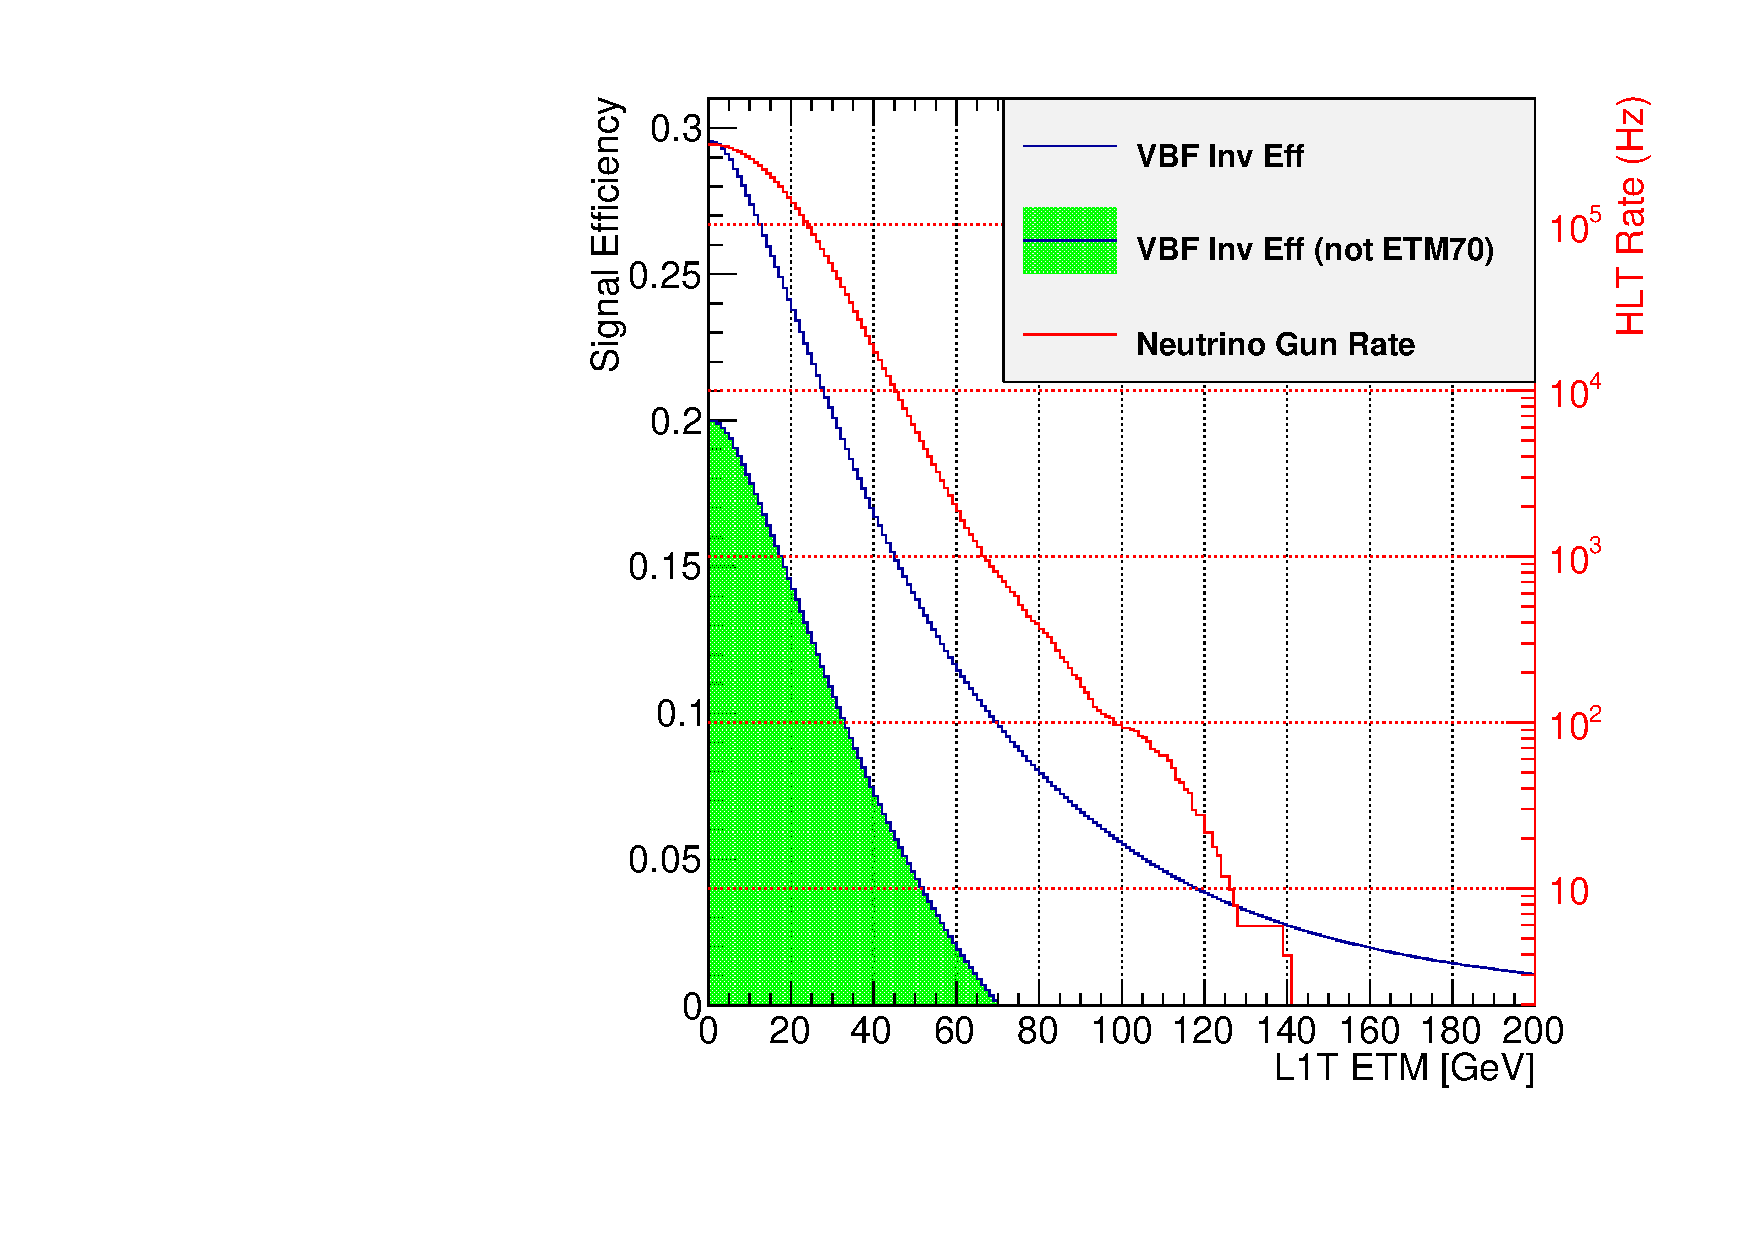
\includegraphics[width=0.49\linewidth]{Chapter08/TriggerStudies/L1T/DijetVBF30_DEta3p5_-_l1t_etm.pdf}}
\subfloat[][]{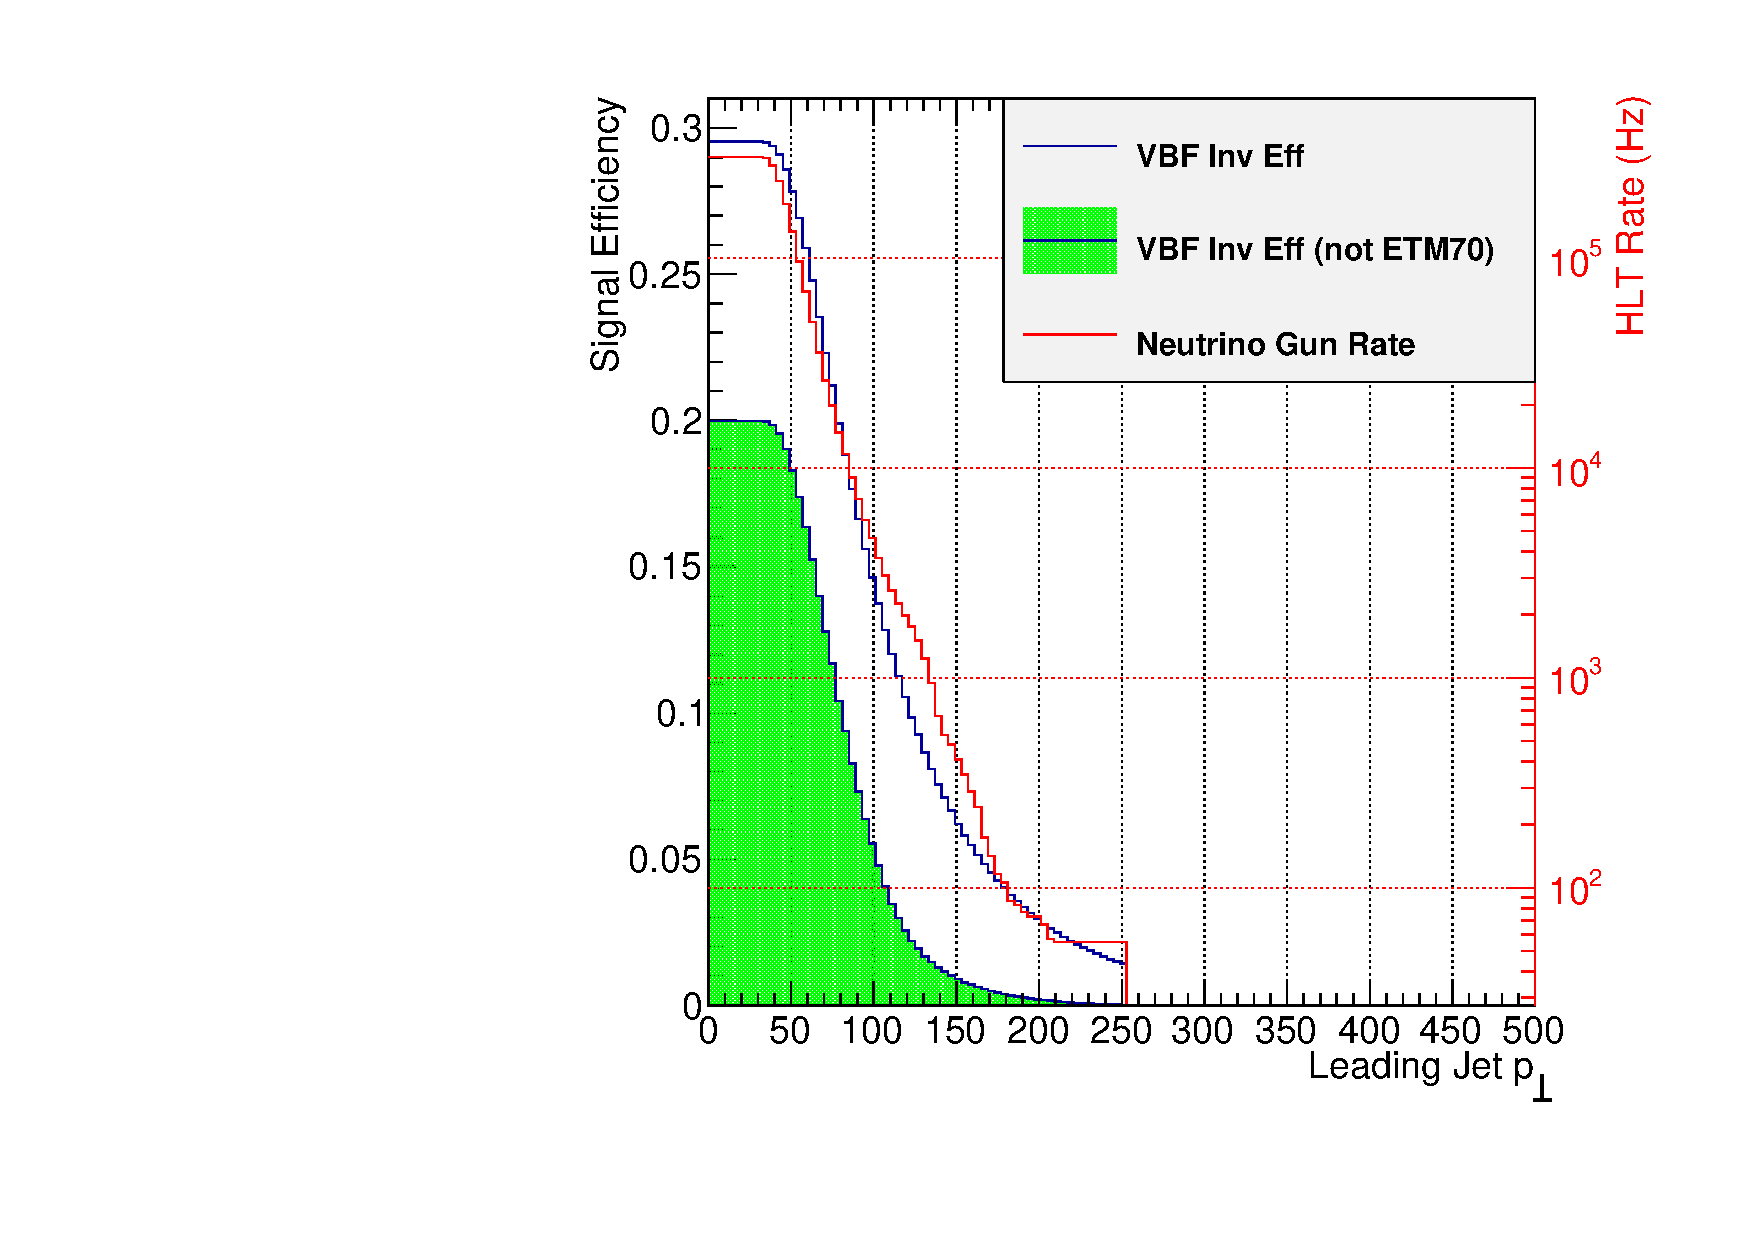
\includegraphics[width=0.49\linewidth]{Chapter08/TriggerStudies/L1T/DijetVBF30_DEta3p5_-_dijet_pt0.pdf}}\\
\caption{Plots produced by the optimization process of possible \gls{L1T} algorithms with a maximum rate of $5\,\kilo\hertz$ for the \textit{\gls{TSG} high luminosity scenario}. Both figures require events with at least one dijet in opposite sides of the detector passing $\pt^{jets}>30$ and $\Delta\eta>3.5$. Figure (a) shows the scan over \gls{L1T} \gls{MET} while figure (b) shows the scan over leading jet \pt. The red line is the estimated rate in $\hertz$, the blue line the faction of accepted signal and the green shaded area the additional efficiency relative to L1\_ETM70.}
\label{FIGURE:RunIIPreparation_L1TAlgorithmDevelopment_VariableScan}
\end{figure}

%%%%%%%%%%%%%%%%%%%%%%%%%%%%%%%%%%%%%%%%%%%%%%%%%%%%%%%%%%%%%%%%%%%%%%%%%%%%%%%%%%%%%%%
%%% SUBSECTION
%%%%%%%%%%%%%%%%%%%%%%%%%%%%%%%%%%%%%%%%%%%%%%%%%%%%%%%%%%%%%%%%%%%%%%%%%%%%%%%%%%%%%%%
\subsection{HLT algorithm development}
\label{SECTION:RunIITriggerStudies_HLTAlgorithmDevelopment}

%Status: DONE (reviewed J.Pela x1)

In the \gls{HLT} trigger menu, the reference trigger was selected as the lowest unprescaled \gls{PF} \gls{MET} trigger available which was \verb|HLT_PFMET170_NoiseCleaned|. This algorithm is seeded by \verb|L1_ETM70| and selects events with \gls{HLT} \gls{PF} \gls{MET} over $170\,\GeV$, which is calculated in the full $\eta$ coverage of the detector. This trigger was calculated to have an expected \gls{HLT} pure rate of $\approx 4.5\,\hertz$ and a signal collection efficiency of 9.4\%, while the Run I prompt trigger efficiency was $\approx 7.6\%$ and the parked trigger between $\approx 10.0\%$ and $\approx 12.9\%$ depending on the acquisition era. 

Similarly to the \gls{L1T} search algorithm, an automatic approach was developed to obtain the best possible algorithm thresholds. In this case, the only variable scanned to fulfil the desired rate algorithm was \gls{HLT} \gls{PF} \gls{MET}. A \textit{grid search} method was implemented, where all possible base configurations of thresholds were tested. For each set of thresholds, the signal efficiency, selection rates, and additional efficiency to reference \gls{HLT} path were calculated. 

Events were selected when at least one \gls{HLT} dijet was found, where both jets were on opposite sides of the detector (\gls{VBF} condition) passing all the requirements of the base selection and the additional \gls{PF} \gls{MET} minimum. The following base configuration variables and values were tested:

\begin{itemize}
  \item Symmetric dijet $p_T^{jets}>{40,50,60}$
  \item Asymmetric dijet $p_T^{jet_1},p_T^{jet_2}>{(50,40),(60,40),(70,40),(80,40),(90,40),(100,40)}$
  \item Dijet $M_{jj}>{500,600,700,800,900,1000,1100}$
  \item Dijet $\Delta\eta>{3.5,3.7,3.9,4.1,4.3,4.5}$
\end{itemize}

The \gls{PF} \gls{MET} minimum threshold was optimised for the signal \gls{HLT} path considering a conservative low target rate of $\approx 1.5\,\hertz$ and an aggressive high target rate  of $5.0\,\hertz$. The assumption was that the high target rate trigger would be the base of the proposal to the \gls{TSG} group, but if there was limited available bandwidth in the menu we would have the fallback conservative trigger proposal. For the sake of brevity, and as the high rate scenario was accepted by the \gls{TSG} group only these results are shown in the following section.

%%%%%%%%%%%%%%%%%%%%%%%%%%%%%%%%%%%%%%%%%%%%%%%%%%%%%%%%%%%%%%%%%%%%%%%%%%%%%%%%%%%%%%%
%%% SUBSUBSECTION
%%%%%%%%%%%%%%%%%%%%%%%%%%%%%%%%%%%%%%%%%%%%%%%%%%%%%%%%%%%%%%%%%%%%%%%%%%%%%%%%%%%%%%%
\subsubsection{Signal path with L1T seed L1\_ETM70}
\label{SECTION:RunIITriggerStudies_HLTAlgorithmDevelopment_L1ETM70}

%Status: DONE (reviewed J.Pela x1)

The baseline \gls{HLT} signal path was optimized for events passing the already available \gls{L1T} reference algorithm which was \verb|L1_ETM70|. All the obtained paths for a $5\,\hertz$ maximum \gls{HLT} rate have significantly lower signal collection efficiency than the reference \gls{HLT} path. Table \ref{TABLE:RunIIPreparation_HLT_Seed_L1TETM70} shows the best algorithm thresholds for the maximum total signal efficiency, maximum additional signal efficiency and lowest lowest \gls{PF} \gls{MET} threshold. For each category of results, the best dijet symmetric and asymmetric \pt thresholds results are presented.

\begin{table}[!htb]
\centering
\resizebox{1.00\linewidth}{!}{
\begin{tabular}{|c|c|c|c|c|c|c|c|c|}
\hline
Algorithm & \multicolumn{5}{c|}{Event Requirements} & Rate & \multicolumn{2}{c|}{Signal Efficiency} \\
\hline
Type       & $p_T^{jet_1},p_T^{jet_2}\,[\GeV]$ & VBF & $\Delta\eta$ & $M_{jj}\,[\GeV]$ & MET $[\GeV]$ & HLT [Hz] & Total [\%] & Additional [\%] \\
\hline\hline
\multicolumn{9}{|c|}{Maximum Total Signal Efficiency} \\
\hline\hline
Asymmetric &                             70,40 & Yes &          3.5 &              500 &          144 &     4.99 &      5.18  &            1.37 \\
Symmetric  &                             40,40 & Yes &          3.5 &              600 &          140 &     4.68 &      5.16  &            1.49 \\
\hline\hline
\multicolumn{9}{|c|}{Maximum Additional Signal Efficiency} \\
\hline\hline
Asymmetric &                             60,40 & Yes &          3.7 &              500 &          140 &     4.84 &      5.13  &            1.55 \\
Symmetric  &                             40,40 & Yes &          3.5 &              600 &          140 &     4.68 &      5.16  &            1.49 \\
\hline\hline
\multicolumn{9}{|c|}{Lowest PF MET Threshold} \\
\hline\hline
Symmetric  &                             60,60 & Yes &          4.1 &              800 &          119 &     4.99 &     $<3\%$ &            1.04 \\
Asymmetric &                            100,40 & Yes &          4.3 &             1000 &          122 &     4.94 &     $<3\%$ &            1.01 \\
\hline
\end{tabular} 
}
\caption{Results of the automatic optimization of possible \gls{HLT} paths for a maximum rate of $5\,\hertz$ for the \textit{\gls{TSG} high luminosity scenario}. All \gls{HLT} algorithms are seeded by L1\_ETM70. Results are presented for the best dijet symmetric and asymmetric \pt thresholds, for maximum total signal efficiency, maximum additional signal efficiency to HLT\_PFMET170\_NoiseCleaned, and lowest \gls{PF} \gls{MET}.}
\label{TABLE:RunIIPreparation_HLT_Seed_L1TETM70}
\end{table}

The best algorithms for both maximum total and additional efficiencies are asymmetric. However, the difference to the best symmetric algorithms is small and comes mostly at a cost of an increased \gls{PF} \gls{MET} requirement or by lowering $M_{jj}$, while increasing the lead jet \pt. The algorithms that minimize \gls{PF} \gls{MET}, have only about $\approx 1\%$ signal efficiency but reduce that threshold by $\approx 50\,\GeV$ when compared with the reference \gls{HLT} path. Plots obtained during the scan of \gls{PF} \gls{MET} for the two maximum additional signal efficiency algorithms can be found in figure \ref{FIGURE:RunIIPreparation_HLT_Seed_L1TETM70}.

\begin{figure}[!htp]
\centering
\subfloat[][]{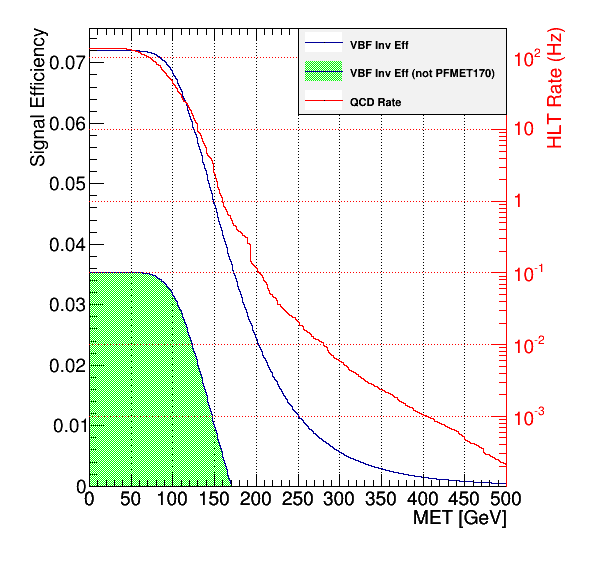
\includegraphics[width=0.45\linewidth]{Chapter08/TriggerStudies/HLT/Seed_L1TETM70/HLT_DijetVBF40-40_DEta3p5_MJJ600}}\qquad
\subfloat[][]{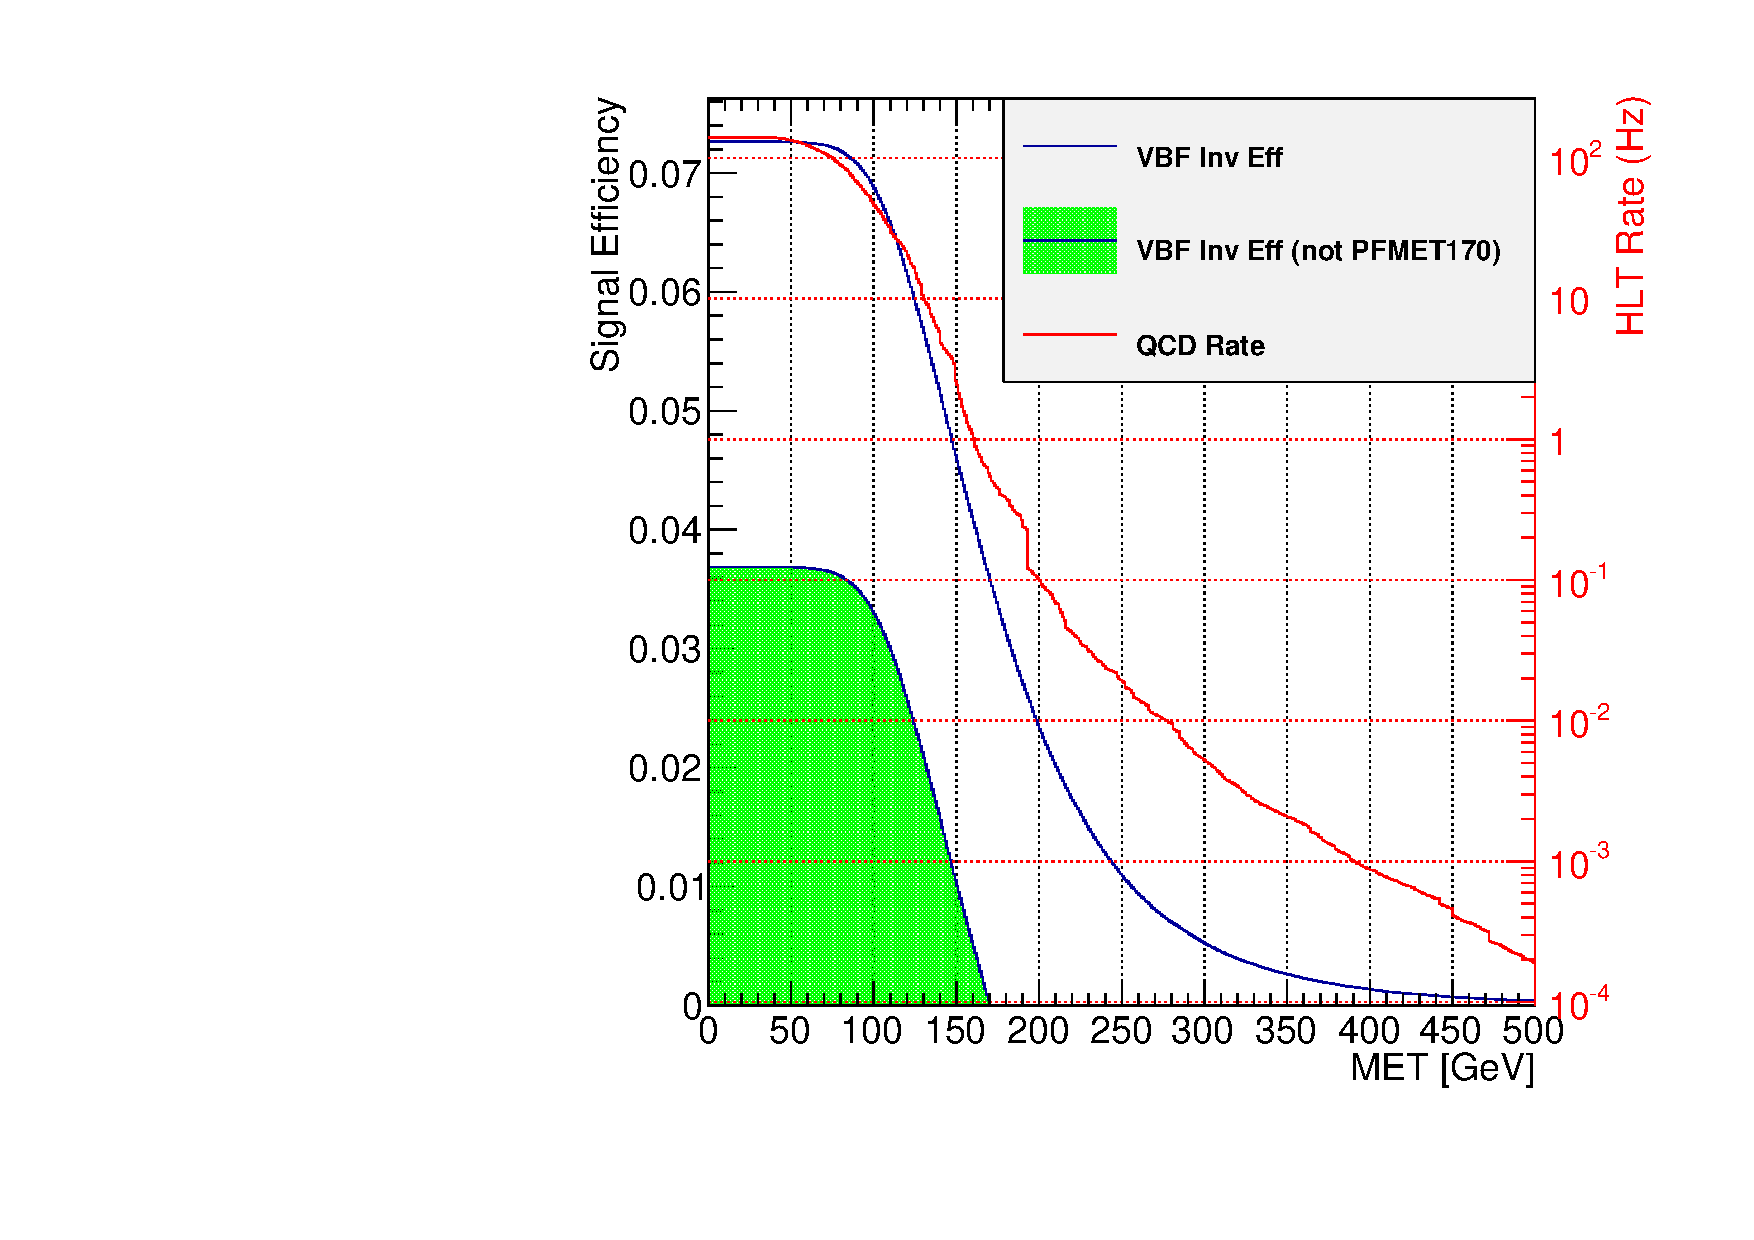
\includegraphics[width=0.45\linewidth]{Chapter08/TriggerStudies/HLT/Seed_L1TETM70/HLT_DijetVBF60-40_DEta3p7_MJJ500}}\\
\caption{Plots showing the scan over \gls{HLT} \gls{PF} \gls{MET} for different algorithm base selection in the \textit{\gls{TSG} high luminosity scenario}. All \gls{HLT} algorithms are seeded by L1\_ETM70. Figure (a) base configuration requiring a dijet on opposite sides of the detector, $p_T^{jet_1},p_T^{jet_2}>40,40\,\GeV$, $\Delta\eta>3.5$ and $M_{jj}>600\,\GeV$ while figure (b) base configuration requiring a dijet on opposite sides of the detector, $p_T^{jet_1},p_T^{jet_2}>60,40\,\GeV$, $\Delta\eta>3.7$ and $M_{jj}>500\,\GeV$.}
\label{FIGURE:RunIIPreparation_HLT_Seed_L1TETM70}
\end{figure}

Since the difference was small between these two trigger paths, for simplicity the symmetric path was chosen. This dedicated trigger, combined with the \gls{HLT} reference trigger, records 10.9\% of the simulated signal process, which corresponds to an increase of signal collection efficiency of 15.8\% when compared with just the reference trigger. Due to the lack of time and manpower to study and implement a new \gls{L1T} algorithm, this was the proposed solution for data taking during 2015. This proposal was accepted by the \gls{TSG} and the resulting \gls{HLT} trigger path used \gls{PF} $\text{MET}_{no-\mu}$, which does not increase the rate significantly. It was integrated into the standard \gls{CMS} trigger menu and was used to record data during the full 2015 Run II campaign.

%%%%%%%%%%%%%%%%%%%%%%%%%%%%%%%%%%%%%%%%%%%%%%%%%%%%%%%%%%%%%%%%%%%%%%%%%%%%%%%%%%%%%%%
%%% SUBSUBSECTION
%%%%%%%%%%%%%%%%%%%%%%%%%%%%%%%%%%%%%%%%%%%%%%%%%%%%%%%%%%%%%%%%%%%%%%%%%%%%%%%%%%%%%%%
\subsubsection{VBF Higgs to invisible trigger turn ons}
\label{SECTION:RunIITriggerStudies_HLTAlgorithmDevelopment_TriggerTurnOns}

In the end of the 2015 data taking run, trigger analysis was performed with the full luminosity recorded with $8\,\TeV$. To study the trigger efficiency in an unbiased way events were used that were recorded through a single muon trigger. The \gls{VBF} Higgs to invisible dedicated \gls{HLT} trigger has requirements in four variables, $\text{MET}_{no-\mu}$, dijet $\pt_T^{jets}$, dijet $\Delta\eta$ and dijet $M_{jj}$. To study the trigger efficiency in selecting events depending on the offline values of these variables (trigger turn ons) they must be analysed individually. 

To decouple the dependency between them, we require all except the one being analysed to be above a threshold where in that specific variable the trigger is 100\% efficient. The offline selection used requires events with lead dijet $p_{T}^{jets}>80\,\GeV$, dijet $M_{jj}>600\,\GeV$, dijet $\Delta\eta_{jj}>3.6$ and $\text{MET}_{no-\mu}>300\,\GeV$. When analysing a variable turn-on, the corresponding event selection requirement is removed. Figure \ref{FIGURE:RunIIPreparation_HLT_TriggerTurnOns} shows the trigger turn ons for all variables used on the trigger as a function of their offline counterparts. 

\begin{figure}[!htp]
\centering
\subfloat[][]{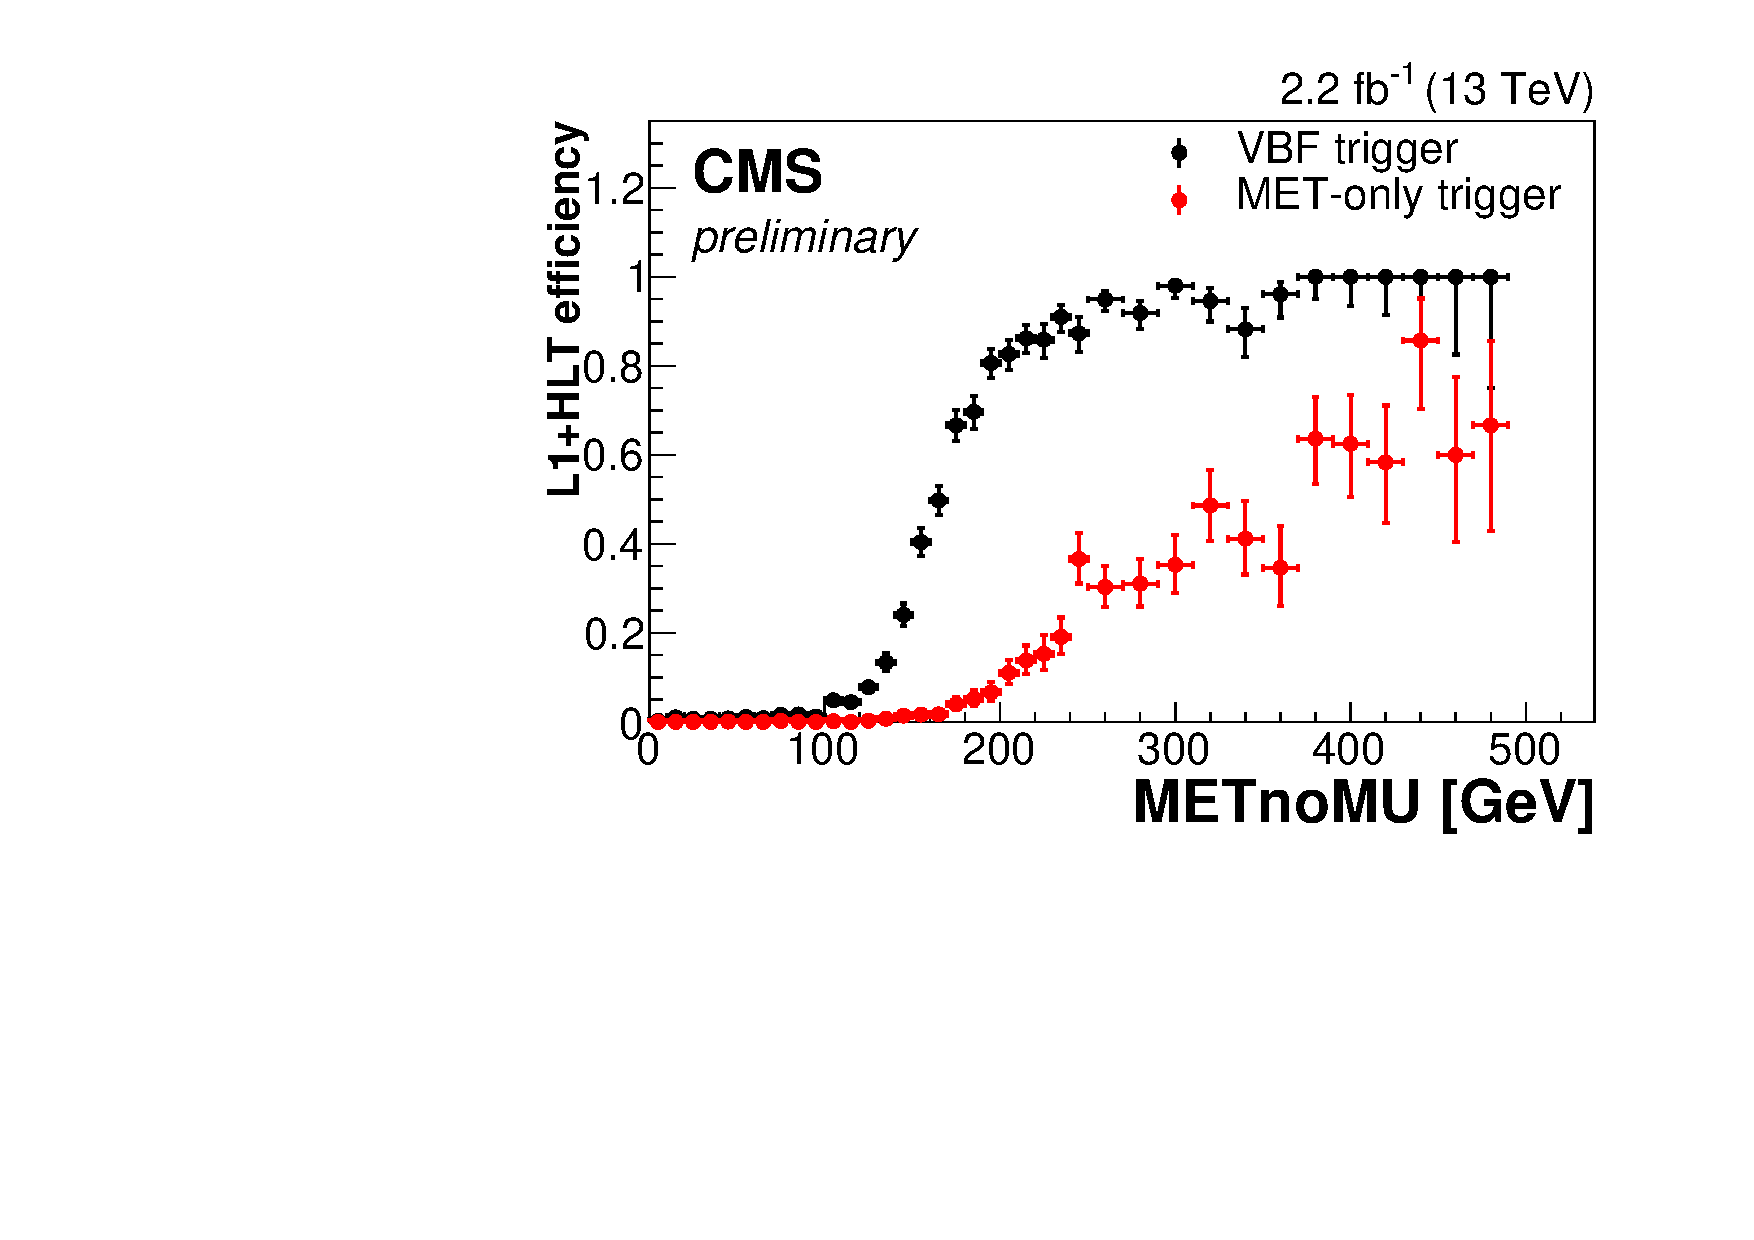
\includegraphics[width=0.49\linewidth]{Chapter08/TriggerStudies/TurnOns/nunu_metnomuons.pdf}}
\subfloat[][]{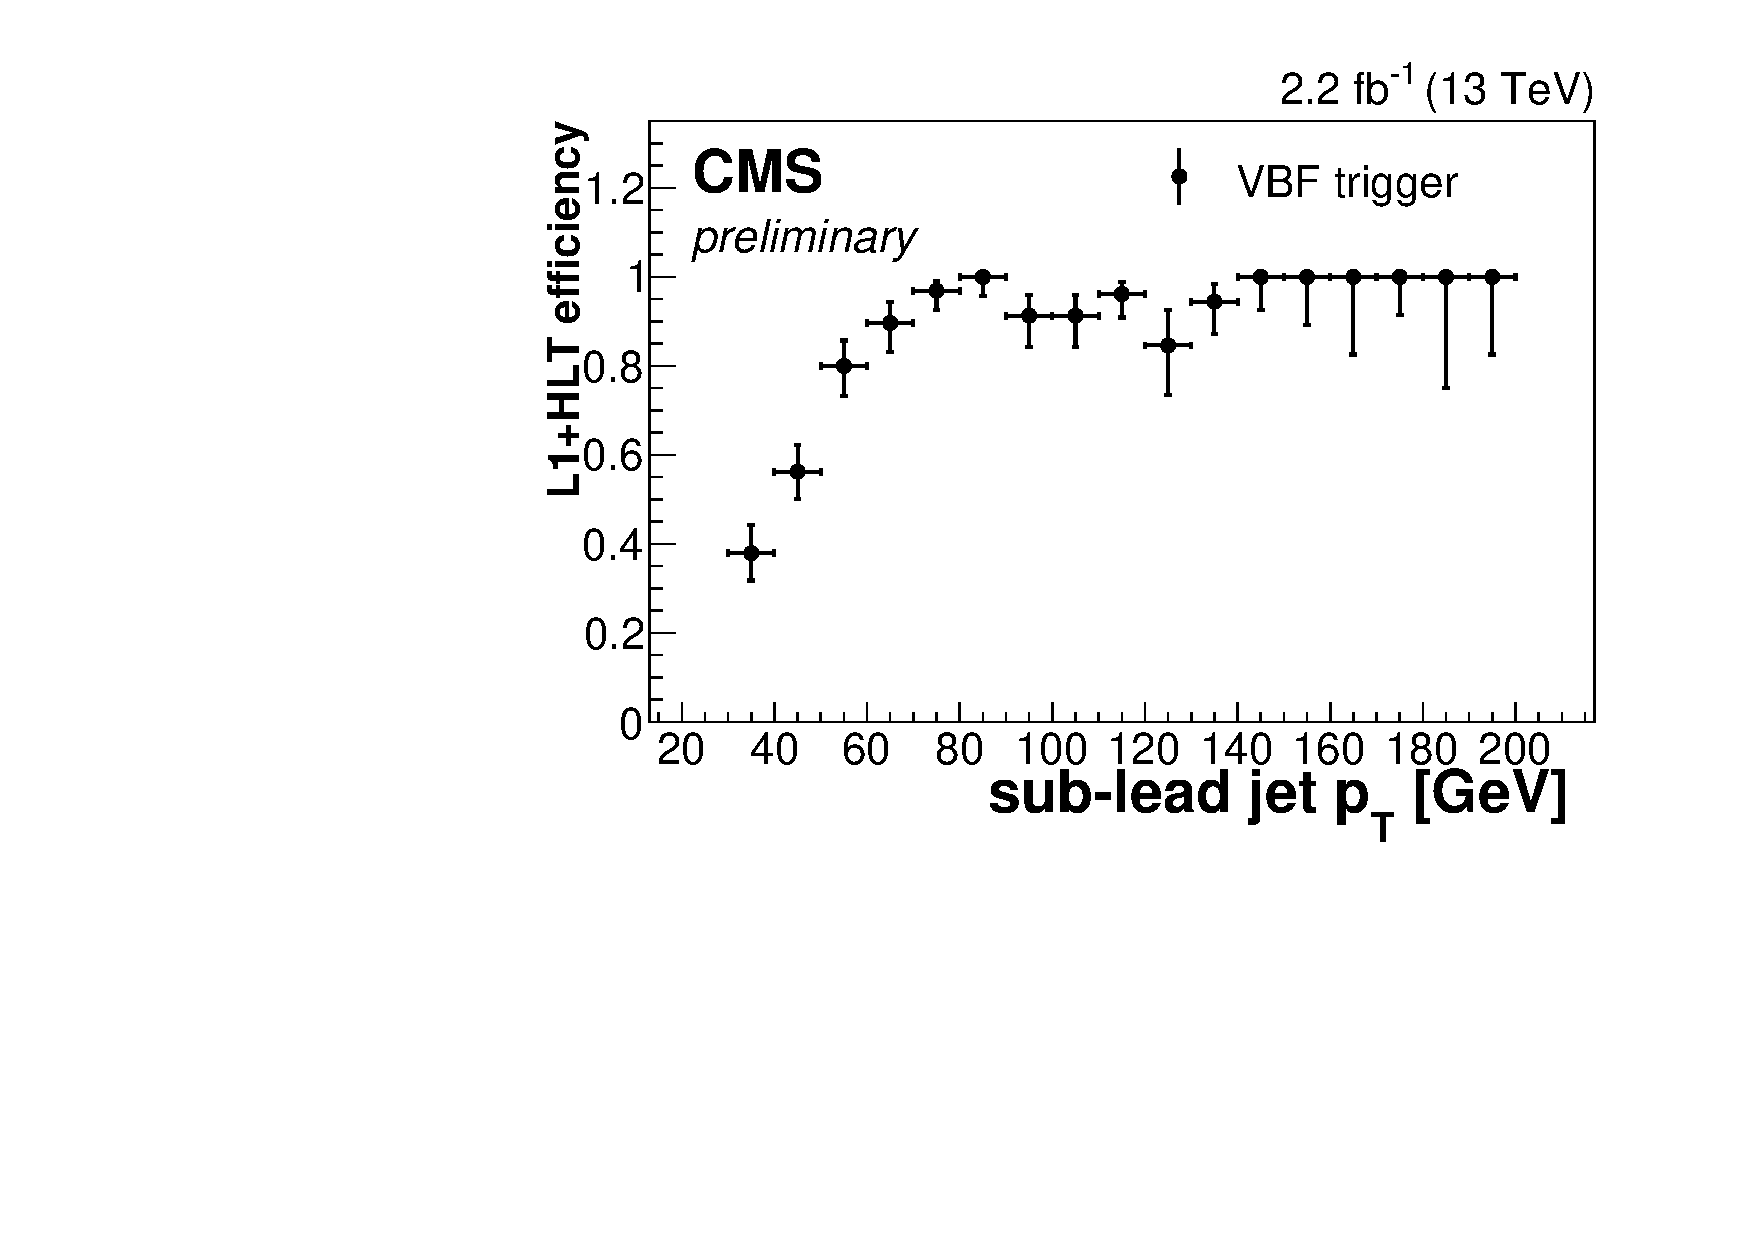
\includegraphics[width=0.49\linewidth]{Chapter08/TriggerStudies/TurnOns/nunu_jet2_pt.pdf}} \\
\subfloat[][]{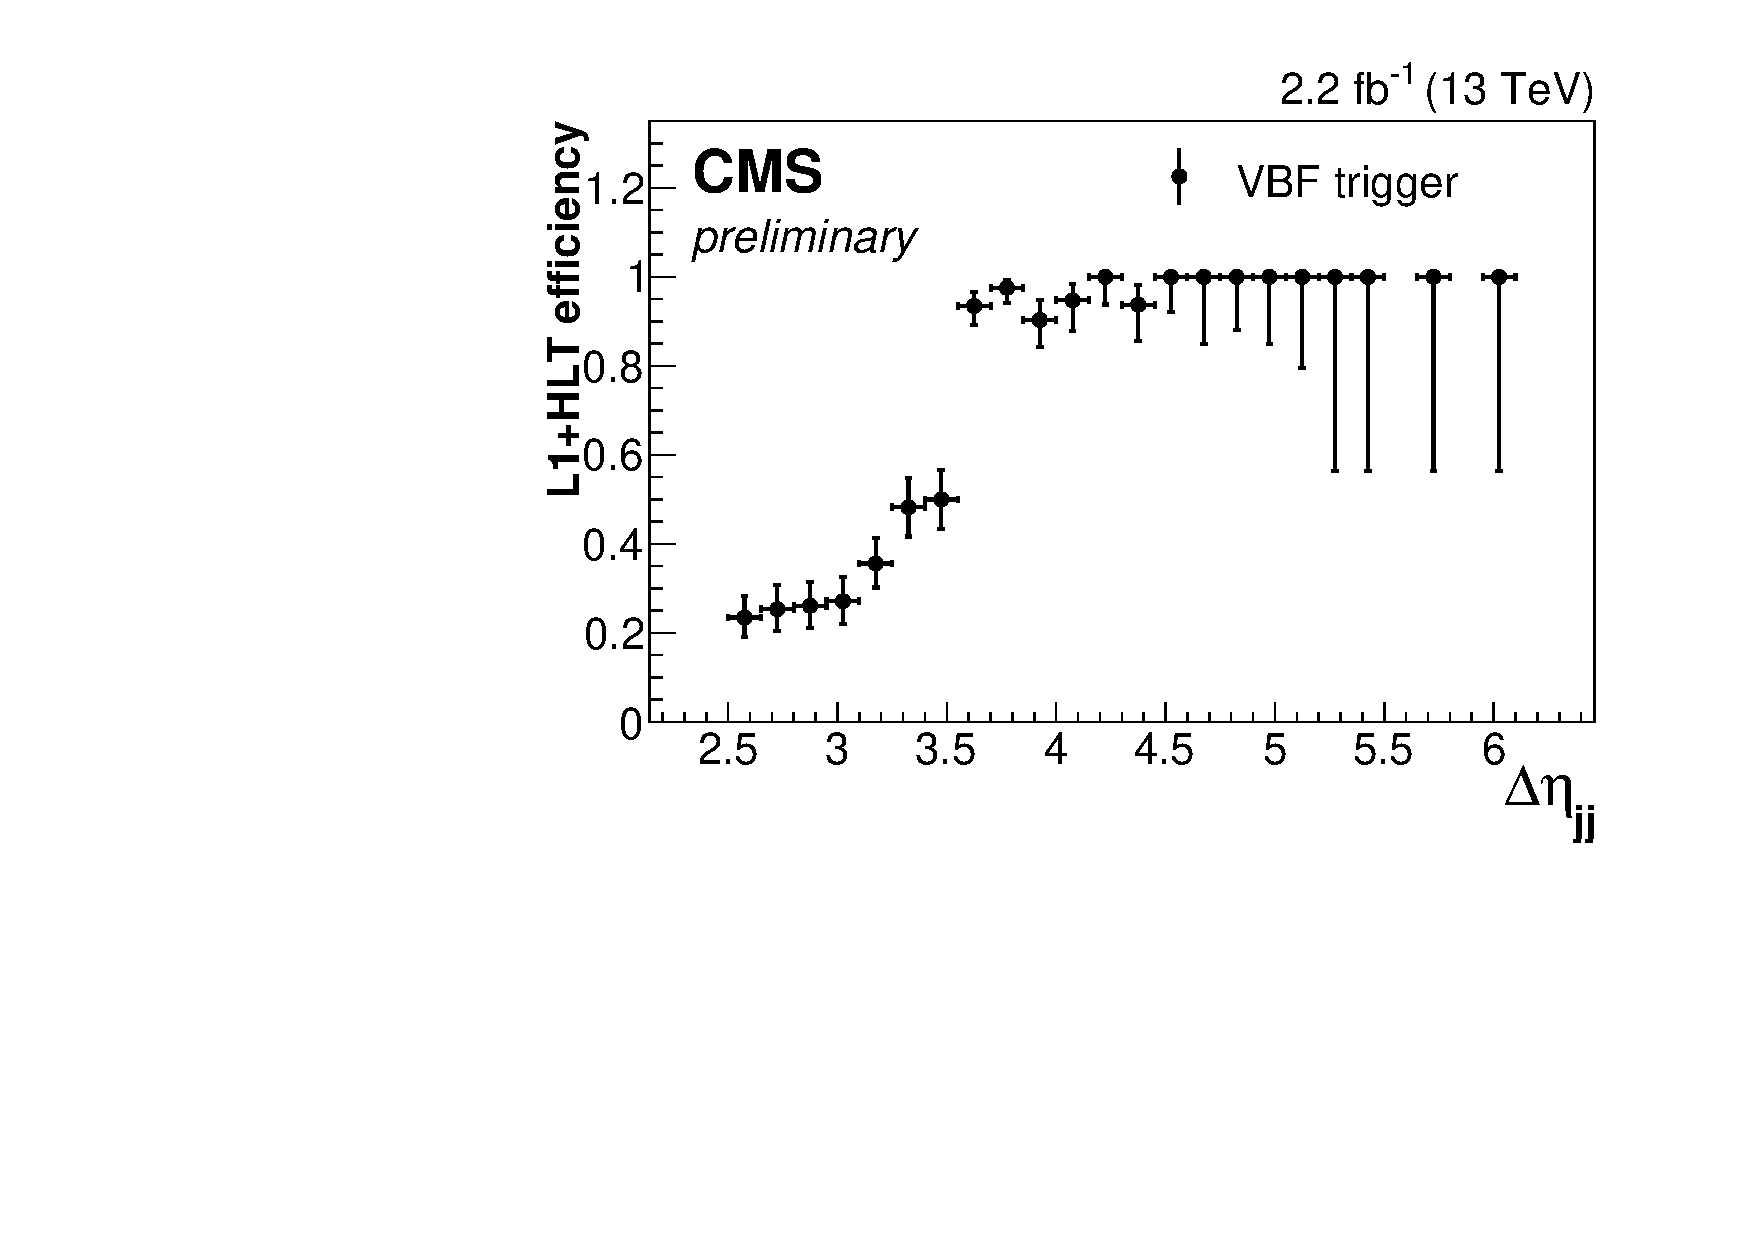
\includegraphics[width=0.49\linewidth]{Chapter08/TriggerStudies/TurnOns/nunu_dijet_deta.pdf}} 
\subfloat[][]{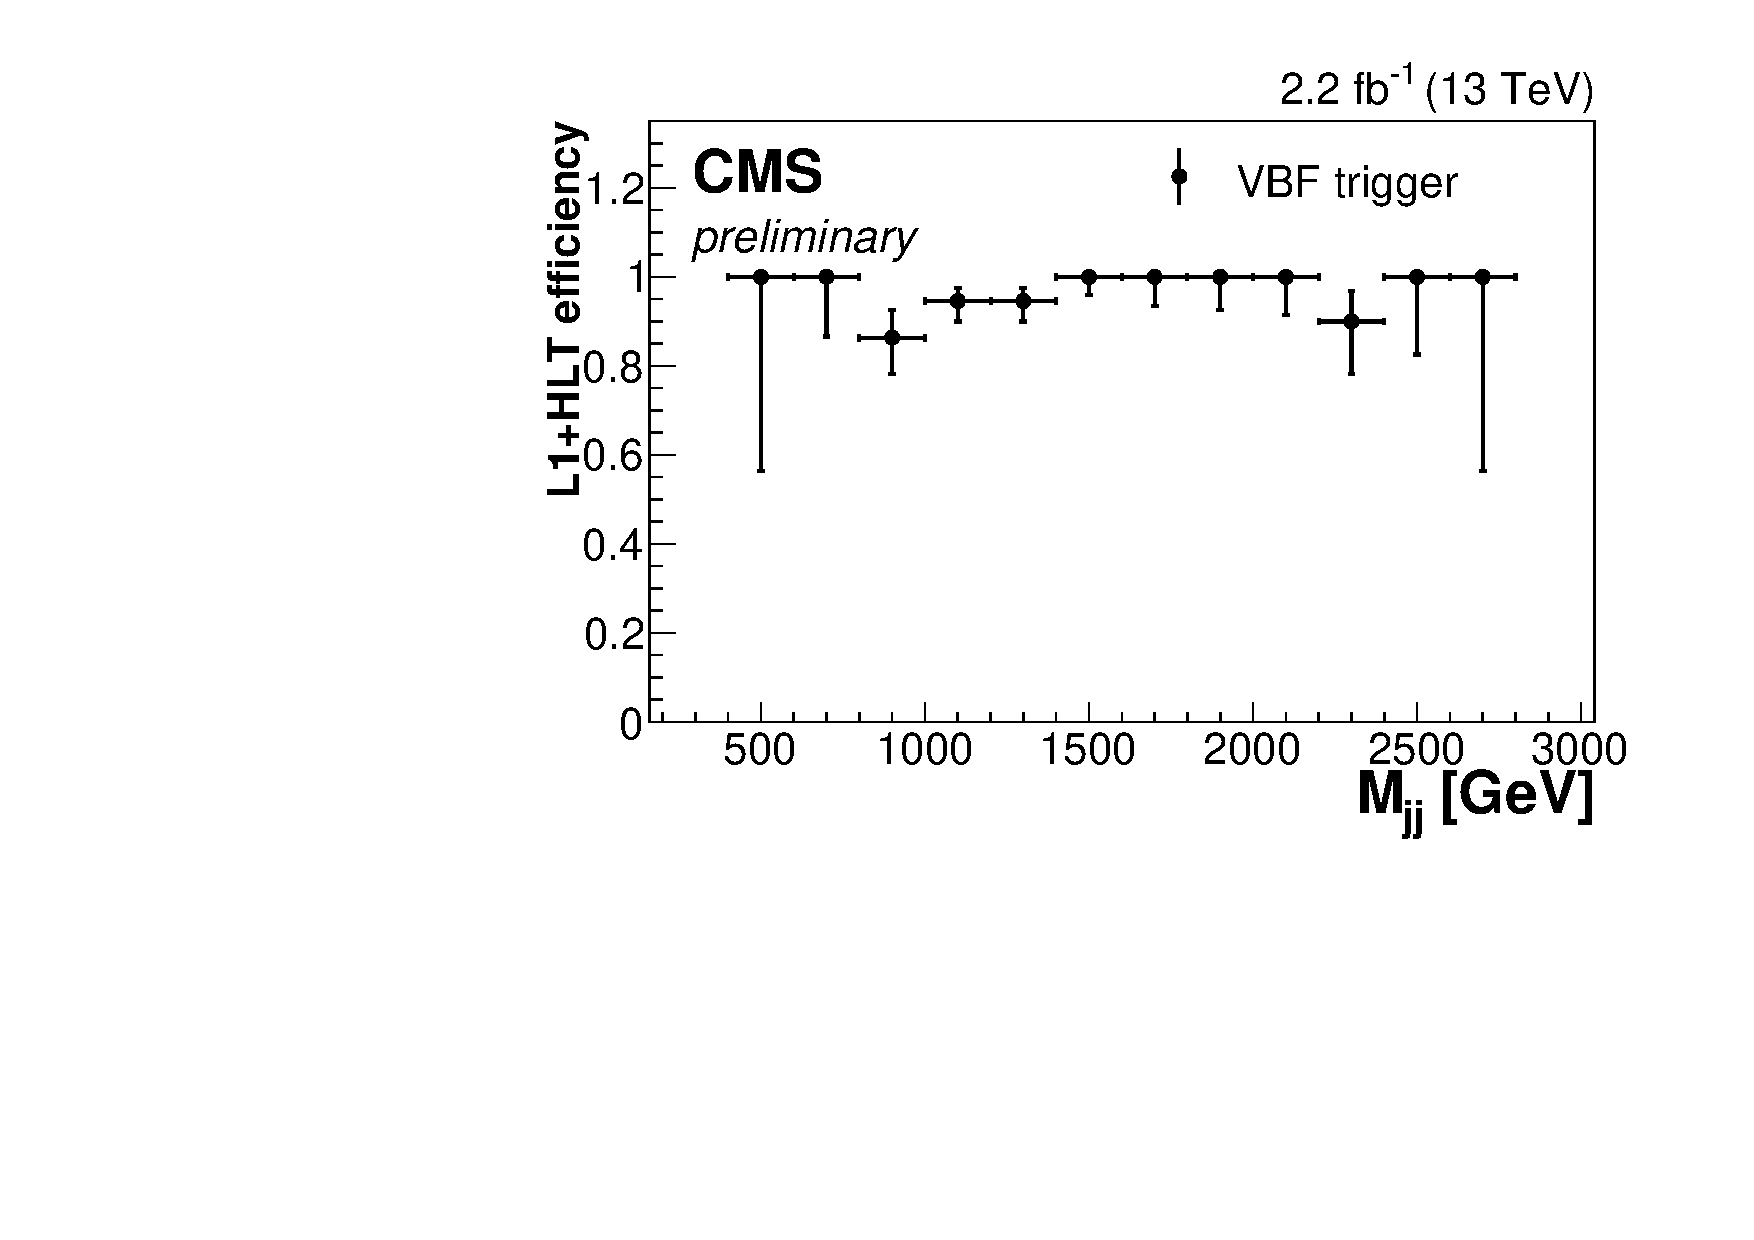
\includegraphics[width=0.49\linewidth]{Chapter08/TriggerStudies/TurnOns/nunu_dijet_M.pdf}} \\
\caption{Trigger turn ons for the \gls{VBF} Higgs to invisible dedicated trigger for (a) $\text{MET}_{no-\mu}$ (includes comparison with the trigger menu \gls{MET} only trigger), (b) dijet sub-lead jet \pt, (c) dijet $\Delta\eta_{jj}$ and (d) dijet $M_{jj}$~\cite{IMAGEREF:LHCJamboree}.}
\label{FIGURE:RunIIPreparation_HLT_TriggerTurnOns}
\end{figure}

It can be seen that the dedicated trigger preforms significantly better than the \gls{MET} only trigger which selects events with \gls{PF} $\text{MET}>170\,\GeV$, when considering the $\text{MET}_{no-\mu}$ turn-on. In this variable, 90\% efficiency is reached at around 
$240\,\GeV$, for the dijet sub-leading jet $\pt$ around $70\,\GeV$, for dijet $\Delta\eta_{jj}$ around 3.7. For dijet $M_{jj}$ a precise turn on cannot be described with the current statistics, but it appears to sharply rise to 100\% just after the trigger requirement of $600\,\GeV$. With these results we can conclude that the trigger is performing as expected and is significantly better than the \gls{MET}-only trigger, considering the analysis needs.

%%%%%%%%%%%%%%%%%%%%%%%%%%%%%%%%%%%%%%%%%%%%%%%%%%%%%%%%%%%%%%%%%%%%%%%%%%%%%%%%%%%%%%%
%%% SUBSUBSECTION
%%%%%%%%%%%%%%%%%%%%%%%%%%%%%%%%%%%%%%%%%%%%%%%%%%%%%%%%%%%%%%%%%%%%%%%%%%%%%%%%%%%%%%%
\subsubsection{Signal path with L1T seed Dijet + MET}
\label{SECTION:RunIITriggerStudies_HLTAlgorithmDevelopment_L1TDijetMET}

%Status: DONE (reviewed J.Pela x1)

Optimization can also be done for the two new proposed \gls{L1T} seeds. Events are selected with a \gls{L1T} dijet with its jets in opposite sides of the detector where $\pt^{jets}>30\,\GeV$, $\Delta\eta>3.5$ and \gls{L1T} $ETM \geq 50\,\GeV$. The same procedure was applied as described in previous section. Results for the best algorithm threshold combinations for maximum total signal efficiency and lowest \gls{PF} \gls{MET} threshold can be found in table \ref{TABLE:RunIIPreparation_HLT_Seed_L1TDijetMET}. Again, for each category of results, the best dijet symmetric and asymmetric \pt thresholds results are presented.

\begin{table}[!htb]
\centering
\resizebox{1.00\linewidth}{!}{
\begin{tabular}{|c|c|c|c|c|c|c|c|c|}
\hline
Algorithm & \multicolumn{5}{c|}{Event Requirements} & Rate & \multicolumn{2}{c|}{Signal Efficiency} \\
\hline
Type       & $p_T^{jet_1},p_T^{jet_2}\,[\GeV]$ & VBF & $\Delta\eta$ & $M_{jj}\,[\GeV]$ & MET $[\GeV]$ & HLT $[\hertz]$ & Total [\%] & Additional [\%] \\
\hline\hline
\multicolumn{9}{|c|}{Maximum efficiency for jets} \\
\hline\hline
Asymmetric &                             60,40 & Yes &          3.7 &              500 &          144 &           4.76 &     4.59 &            1.57 \\
Symmetric  &                             40,40 & Yes &          3.5 &              600 &          145 &           4.69 &     4.48 &            1.52 \\
\hline\hline
\multicolumn{9}{|c|}{Maximum Additional Efficiency} \\
\hline\hline
Asymmetric &                             60,40 & Yes &          4.1 &              500 &          140 &           4.77 &     4.39 &            1.71 \\
Symmetric  &                             40,40 & Yes &          4.1 &              600 &          141 &           4.95 &     4.23 &            1.62 \\
\hline\hline
\multicolumn{9}{|c|}{Lowest MET Threshold} \\
\hline\hline
Symmetric  &                             60,60 & Yes &          4.5 &             1000 &          122 &           4.93 &     2.28 &            1.02 \\
Asymmetric &                            100,40 & Yes &          4.5 &             1100 &          125 &           4.87 &     2.64 &            1.00 \\
\hline
\end{tabular}
}
\caption{Results of the automatic optimization of possible \gls{HLT} paths for a maximum rate of $5\,\hertz$ for the \textit{\gls{TSG} high luminosity scenario}. All \gls{HLT} algorithms are seeded by proposed \gls{L1T} algorithm selecting a dijet passing requirements \gls{VBF}, $\pt^{jets}>30\,\GeV$, and $\Delta\eta>3.5$ and $ETM \geq 50\,\GeV$. Results are presented for the best dijet symmetric and asymmetric \pt thresholds, for maximum total signal efficiency, maximum additional signal efficiency to HLT\_PFMET170\_NoiseCleaned, and lowest \gls{PF} \gls{MET}.}
\label{TABLE:RunIIPreparation_HLT_Seed_L1TDijetMET}
\end{table}

As expected lowering the \gls{L1T} \gls{MET} threshold allows a bigger additional signal efficiency to be achieved. The best algorithms in this benchmark quantity, similarly to the previous study, also requires \gls{HLT} $\text{MET}>140\,\GeV$  and similar dijet thresholds, implying the added efficiency comes from recovering events that fail \verb|L1_ETM70|. It is also interesting that the total efficiency is lower than seen in table \ref{TABLE:RunIIPreparation_HLT_Seed_L1TETM70}, which could be caused by the additional \gls{L1T} jet requirements. Plots of the two best additional signal efficiency algorithms scans of \gls{PF} \gls{MET} can be found in figure \ref{FIGURE:RunIIPreparation_HLT_Seed_L1TDijetMET}.

\begin{figure}[!htp]%
\subfloat[][]{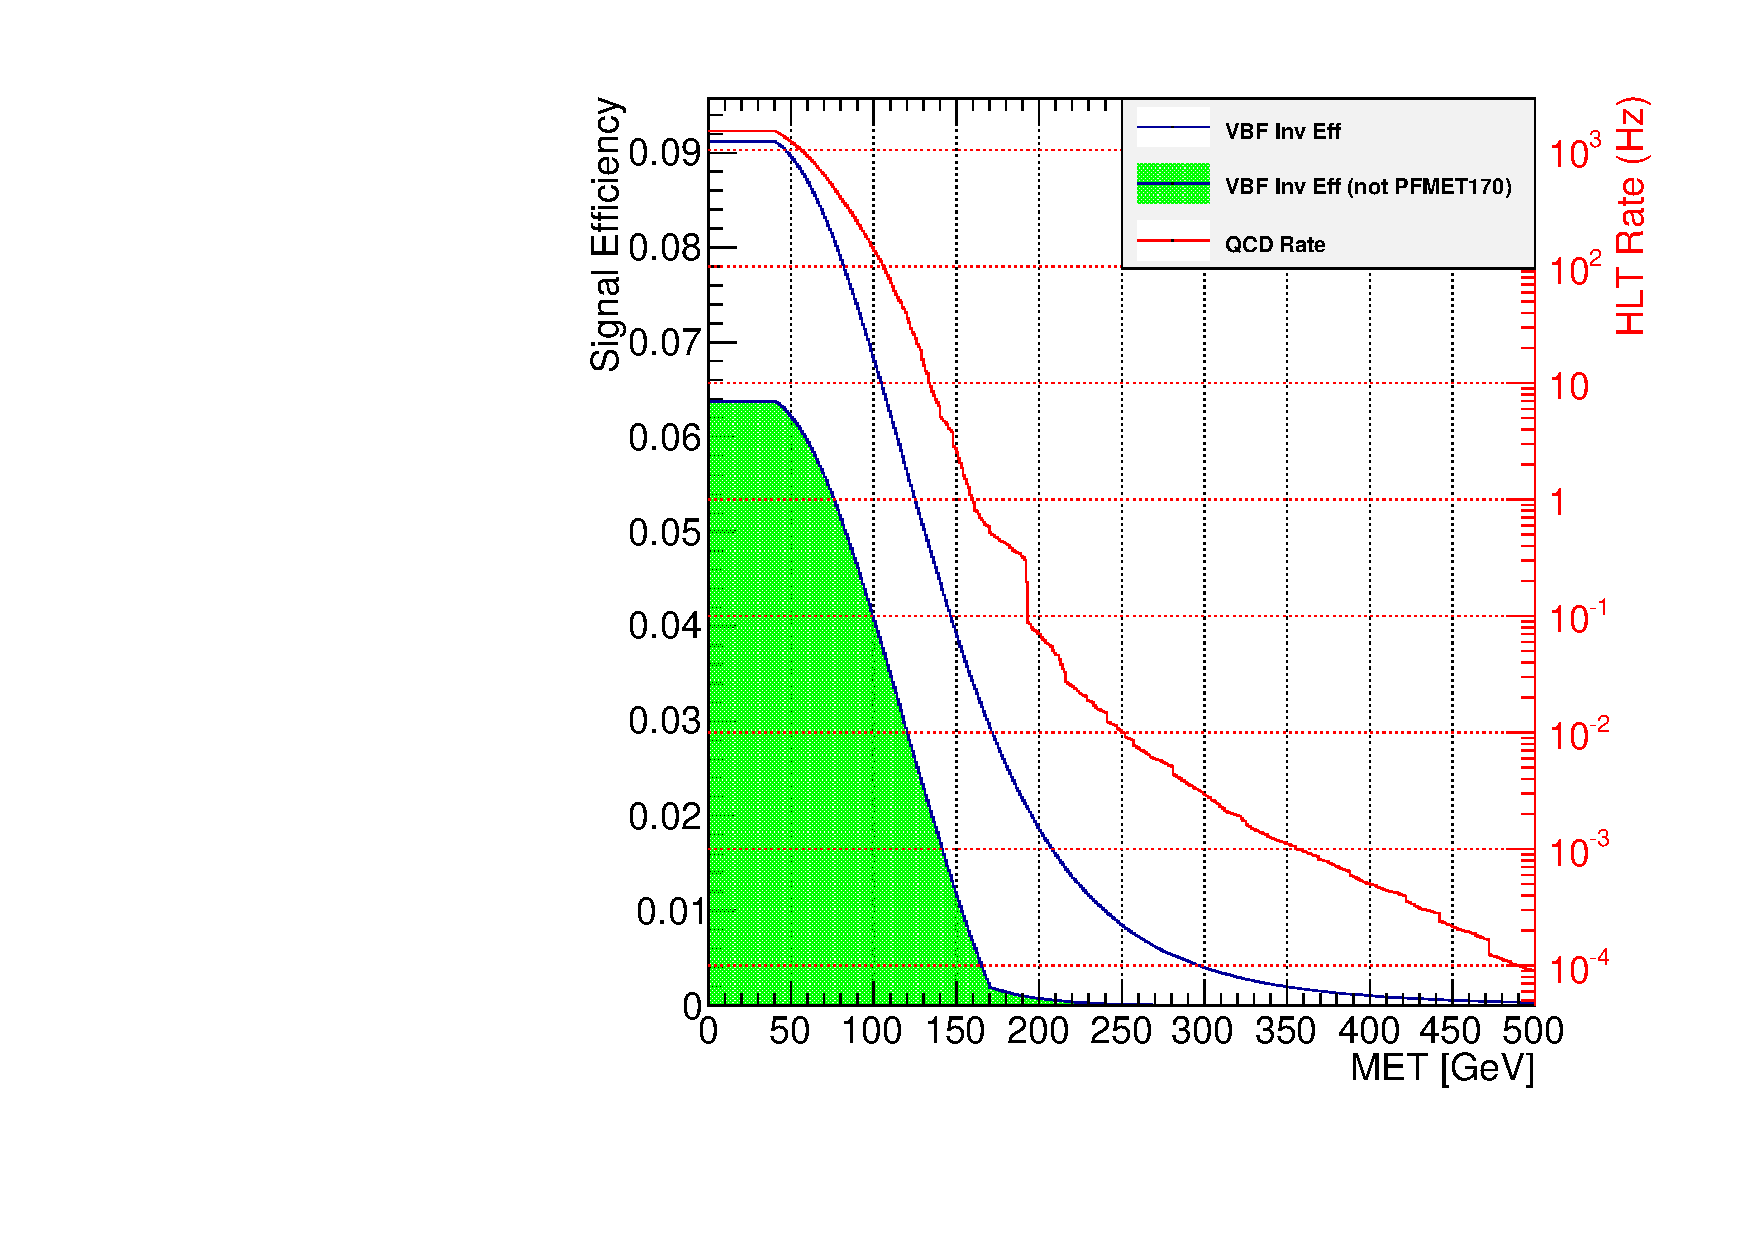
\includegraphics[width=0.45\linewidth]{Chapter08/TriggerStudies/HLT/Seed_DijetVBF30_DEta3p5_ETM50/HLT_DijetVBF60-40_DEta4p1_MJJ500.pdf}}\qquad
\subfloat[][]{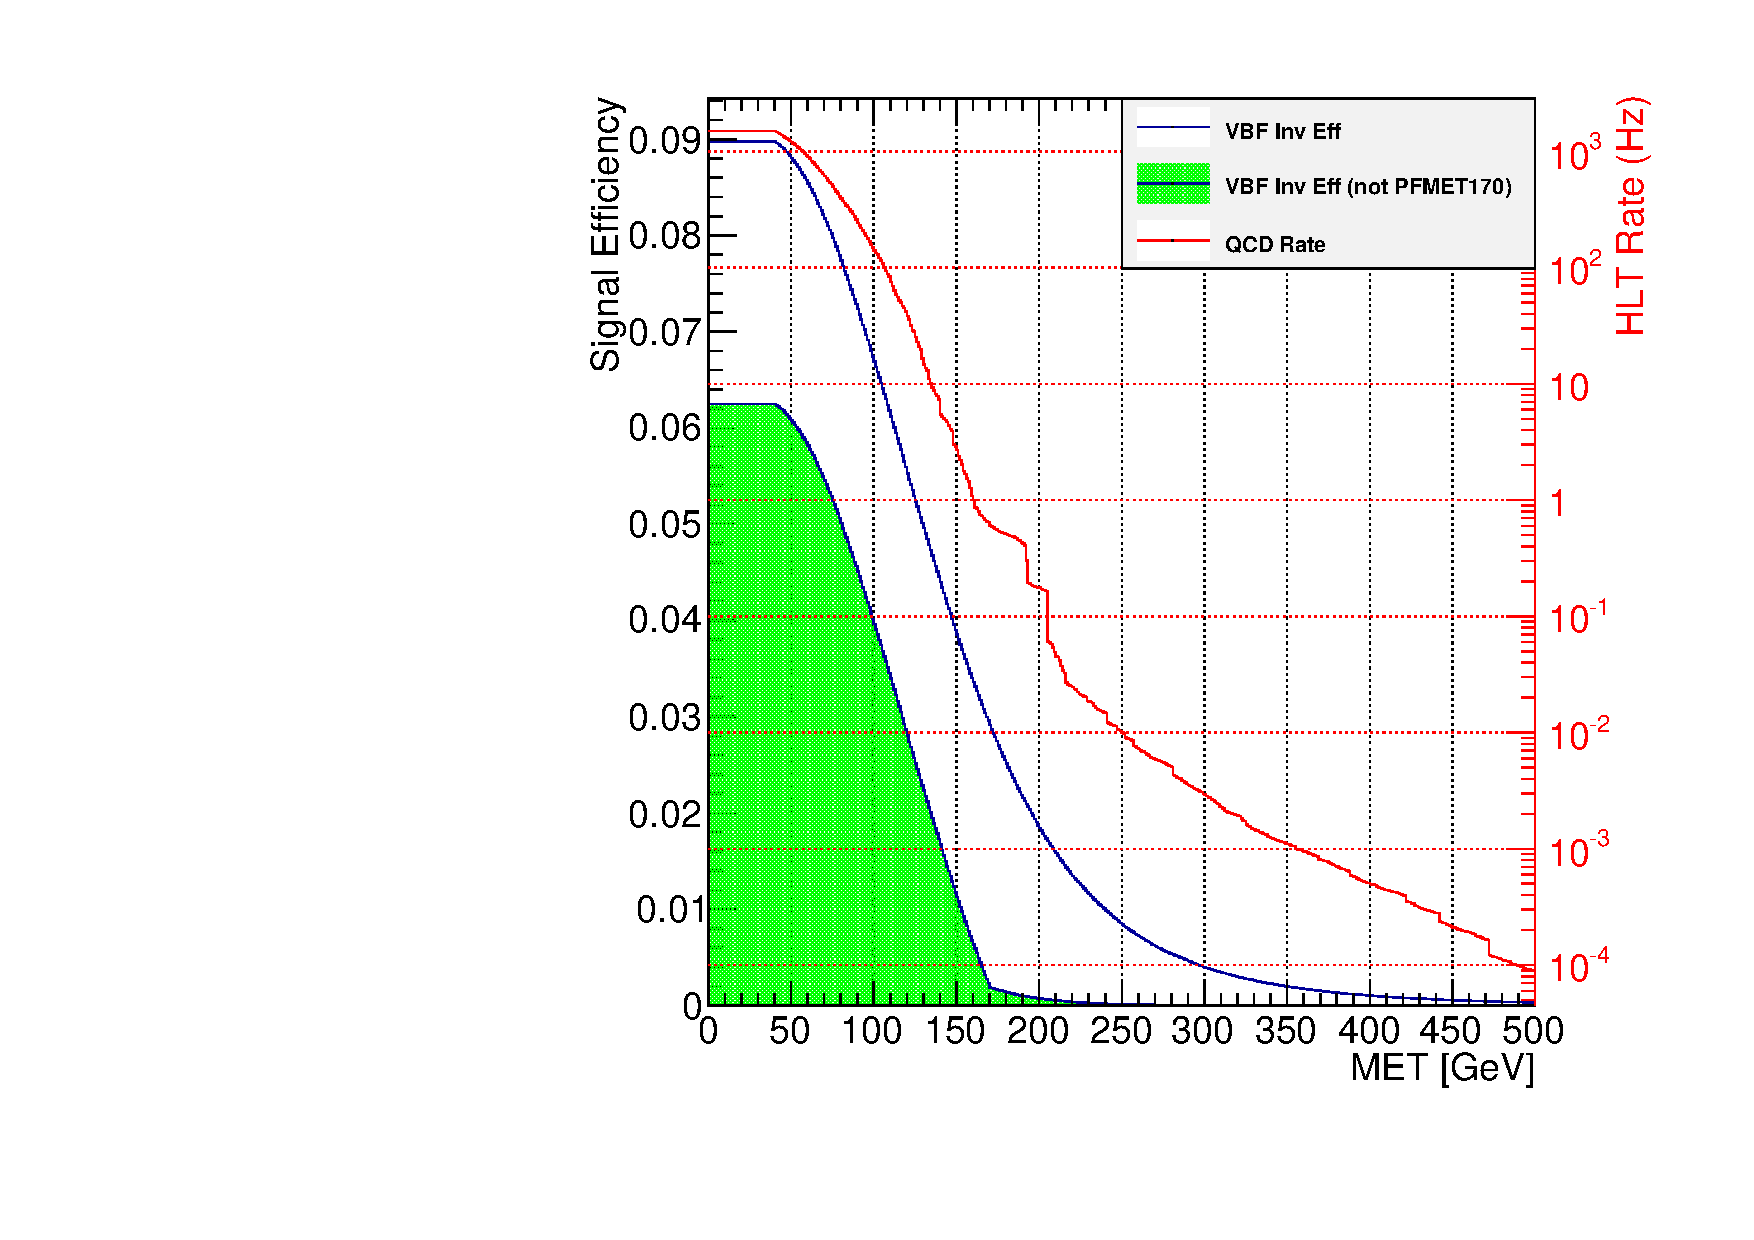
\includegraphics[width=0.45\linewidth]{Chapter08/TriggerStudies/HLT/Seed_DijetVBF30_DEta3p5_ETM50/HLT_DijetVBF40-40_DEta4p1_MJJ600.pdf}}\\
\caption{Plots showing the scan over \gls{HLT} \gls{PF} \gls{MET} for different algorithm base selection in the \textit{\gls{TSG} high luminosity scenario}. All \gls{HLT} algorithms are seeded by proposed \gls{L1T} algorithm selecting a dijet passing requirements \gls{VBF}, $\pt^{jets}>30\,\GeV$, and $\Delta\eta>3.5$ and $ETM \geq 50\,\GeV$. Figure (a) base configuration requiring a dijet on opposite sides of the detector, $p_T^{jet_1},p_T^{jet_2}>60,40\,\GeV$, $\Delta\eta>4.1$ and $M_{jj}>500\,\GeV$ while figure (b) base configuration requiring a dijet on opposite sides of the detector, $p_T^{jet_1},p_T^{jet_2}>40,40\,\GeV$, $\Delta\eta>4.1$ and $M_{jj}>600\,\GeV$.}
\label{FIGURE:RunIIPreparation_HLT_Seed_L1TDijetMET}
\end{figure}

The tail of additional efficiency can be seen continuing above \gls{PF} $\text{MET}>170\,\GeV$, further supporting the hypothesis that efficiency is being recovered from events lost by the \verb|L1_ETM70| requirement. The best additional signal efficiency algorithm optimized for this \gls{L1T} dijet plus \gls{MET} seed combined with the \gls{HLT} reference trigger records 11.11\% of the simulated signal process. This dedicated \gls{HLT} trigger, when compared with the proposed dedicated trigger for Run II, gives 14.8\% additional efficiency with an increase of 2.0\% in total signal efficiency.

%%%%%%%%%%%%%%%%%%%%%%%%%%%%%%%%%%%%%%%%%%%%%%%%%%%%%%%%%%%%%%%%%%%%%%%%%%%%%%%%%%%%%%%
%%% SUBSUBSECTION
%%%%%%%%%%%%%%%%%%%%%%%%%%%%%%%%%%%%%%%%%%%%%%%%%%%%%%%%%%%%%%%%%%%%%%%%%%%%%%%%%%%%%%%
\subsubsection{Signal path with L1T seed Dijet + Single Jet}
\label{SECTION:RunIITriggerStudies_HLTAlgorithmDevelopment_L1TDijetSingleJet}

%Status: DONE (reviewed J.Pela x1)

Finally, optimization of \gls{HLT} algorithms was also preformed over a possible \gls{L1T} seed without any \gls{MET} requirement. This seed selected events with a \gls{L1T} dijet with its jets in opposite sides of the detector, where $\pt^{jets}>30\,\GeV$, $\Delta\eta>3.5$ and the highest \pt \gls{L1T} jet in the event has at least $96\,\GeV$. This high \pt jet can and should be in the selected dijet but for simplicity of algorithm design both in hardware and software coupled with development time constraints, forced these conditions to be kept separated. The same procedure from previous section is applied and the results can be found in table \ref{TABLE:RunIITriggerStudies_HLT_Seed_L1TDijetSingleJet}.

\begin{table}[!htb]
\centering
\resizebox{1.00\linewidth}{!}{
\begin{tabular}{|c|c|c|c|c|c|c|c|c|}
\hline
Algorithm & \multicolumn{5}{c|}{Event Requirements} & Rate & \multicolumn{2}{c|}{Signal Efficiency} \\
\hline
Type       & $p_T^{jet_1},p_T^{jet_2}\,[\GeV]$ & VBF & $\Delta\eta$ & $M_{jj}\,[\GeV]$ & MET $[\GeV]$ & HLT [Hz] & Total [\%] & Additional [\%] \\
\hline\hline
\multicolumn{9}{|c|}{Maximum efficiency} \\
\hline\hline
Symmetric  &                             40,40 & Yes &          3.5 &              500 &          148 &     4.93 &       4.79 &            1.75 \\
Asymmetric &                             50,40 & Yes &          3.5 &              500 &          148 &     4.92 &       4.78 &            1.74 \\
\hline\hline
\multicolumn{9}{|c|}{Maximum Additional Efficiency} \\
\hline\hline
Asymmetric &                             90,40 & Yes &          4.1 &              500 &          140 &     4.51 &       4.44 &            1.86 \\
Symmetric  &                             40,40 & Yes &          4.3 &              800 &          140 &     4.81 &       4.09 &            1.78 \\
\hline\hline
\multicolumn{9}{|c|}{Lowest MET Threshold} \\
\hline\hline
Symmetric  &                             60,60 & Yes &          4.3 &             1100 &          123 &     4.89 &       2.53 &            1.20 \\
Asymmetric &                            100,40 & Yes &          4.3 &             1100 &          128 &     4.98 &       3.18 &            1.42 \\
\hline
\end{tabular}
}
\caption{Results of the automatic optimization of possible \gls{HLT} paths for a maximum rate of $5\,\hertz$ for the \textit{\gls{TSG} high luminosity scenario}. All \gls{HLT} algorithms are seeded by proposed \gls{L1T} algorithm selecting a dijet passing requirements \gls{VBF}, $\pt^{jets}>30\,\GeV$, and $\Delta\eta>3.5$ and a single jet $\pt^{jets}>96\,\GeV$. Results are presented for the best dijet symmetric and asymmetric \pt thresholds, for maximum total signal efficiency, maximum additional signal efficiency to HLT\_PFMET170\_NoiseCleaned, and lowest \gls{PF} \gls{MET}.}
\label{TABLE:RunIITriggerStudies_HLT_Seed_L1TDijetSingleJet}
\end{table}

The best additional signal efficiency \gls{HLT} trigger algorithm found was highly asymmetric, as expected. Surprisingly, this is the best additional efficiency algorithm obtained in all studies. Once again, the determined \gls{PF} \gls{MET} was $140\,\GeV$, suggesting that the recovered efficiency comes from the absence of an \gls{L1T} \gls{MET} restriction, combined with the asymmetric topological requirements. The total efficiency is also below the algorithms based on the \verb|L1_ETM70| seed. Since the best additional efficiency configurations are selected, this implies that phase space lost by reference algorithm is being recovered at the cost of total efficiency. Plots of the two best additional signal efficiency algorithms \gls{PF} \gls{MET} scans can be found in figure \ref{FIGURE:RunIITriggerStudies_HLT_Seed_L1TDijetSingleJet}.

\begin{figure}[!htp]%
\centering
\subfloat[][]{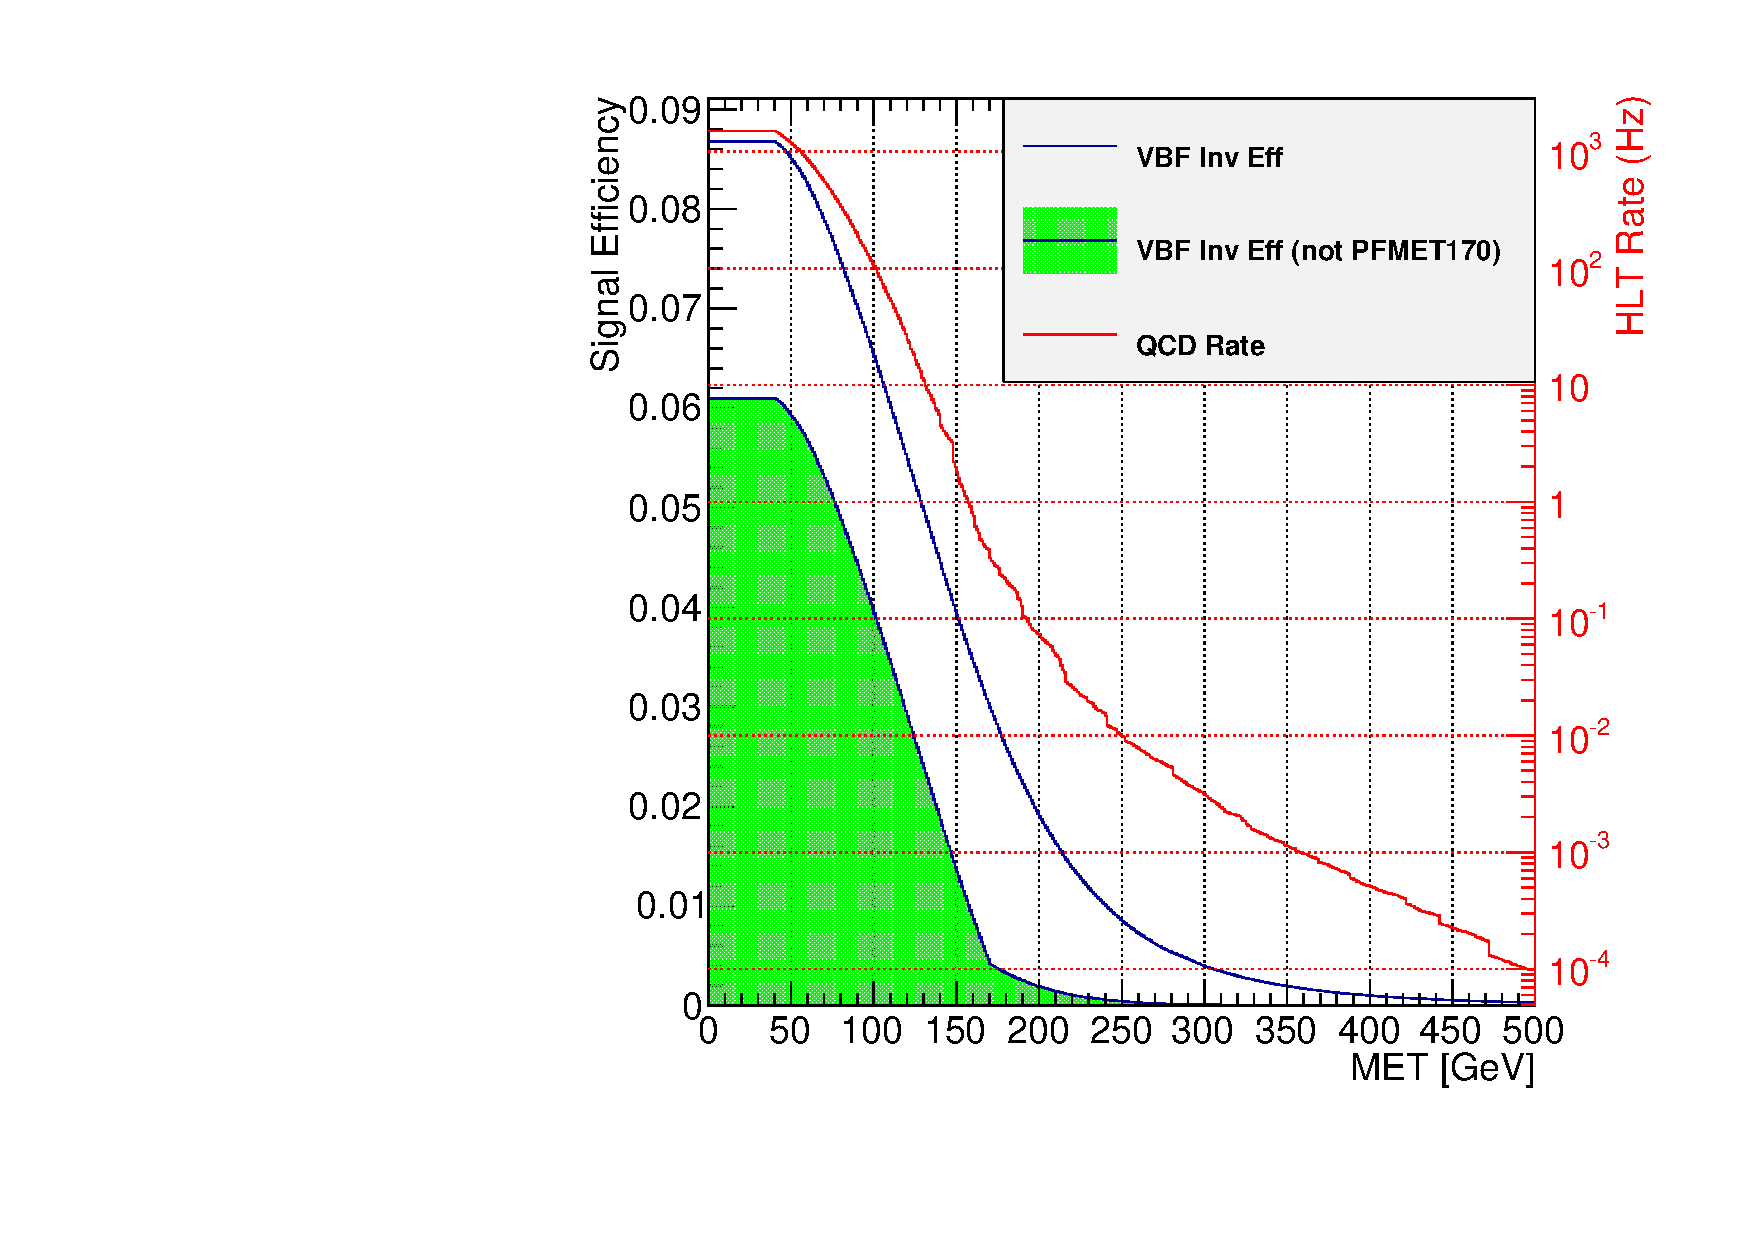
\includegraphics[width=0.45\linewidth]{Chapter08/TriggerStudies/HLT/Seed_DijetVBF30_DEta3p5_SingleJet96/HLT_DijetVBF90-40_DEta4p1_MJJ500.pdf}}\qquad
\subfloat[][]{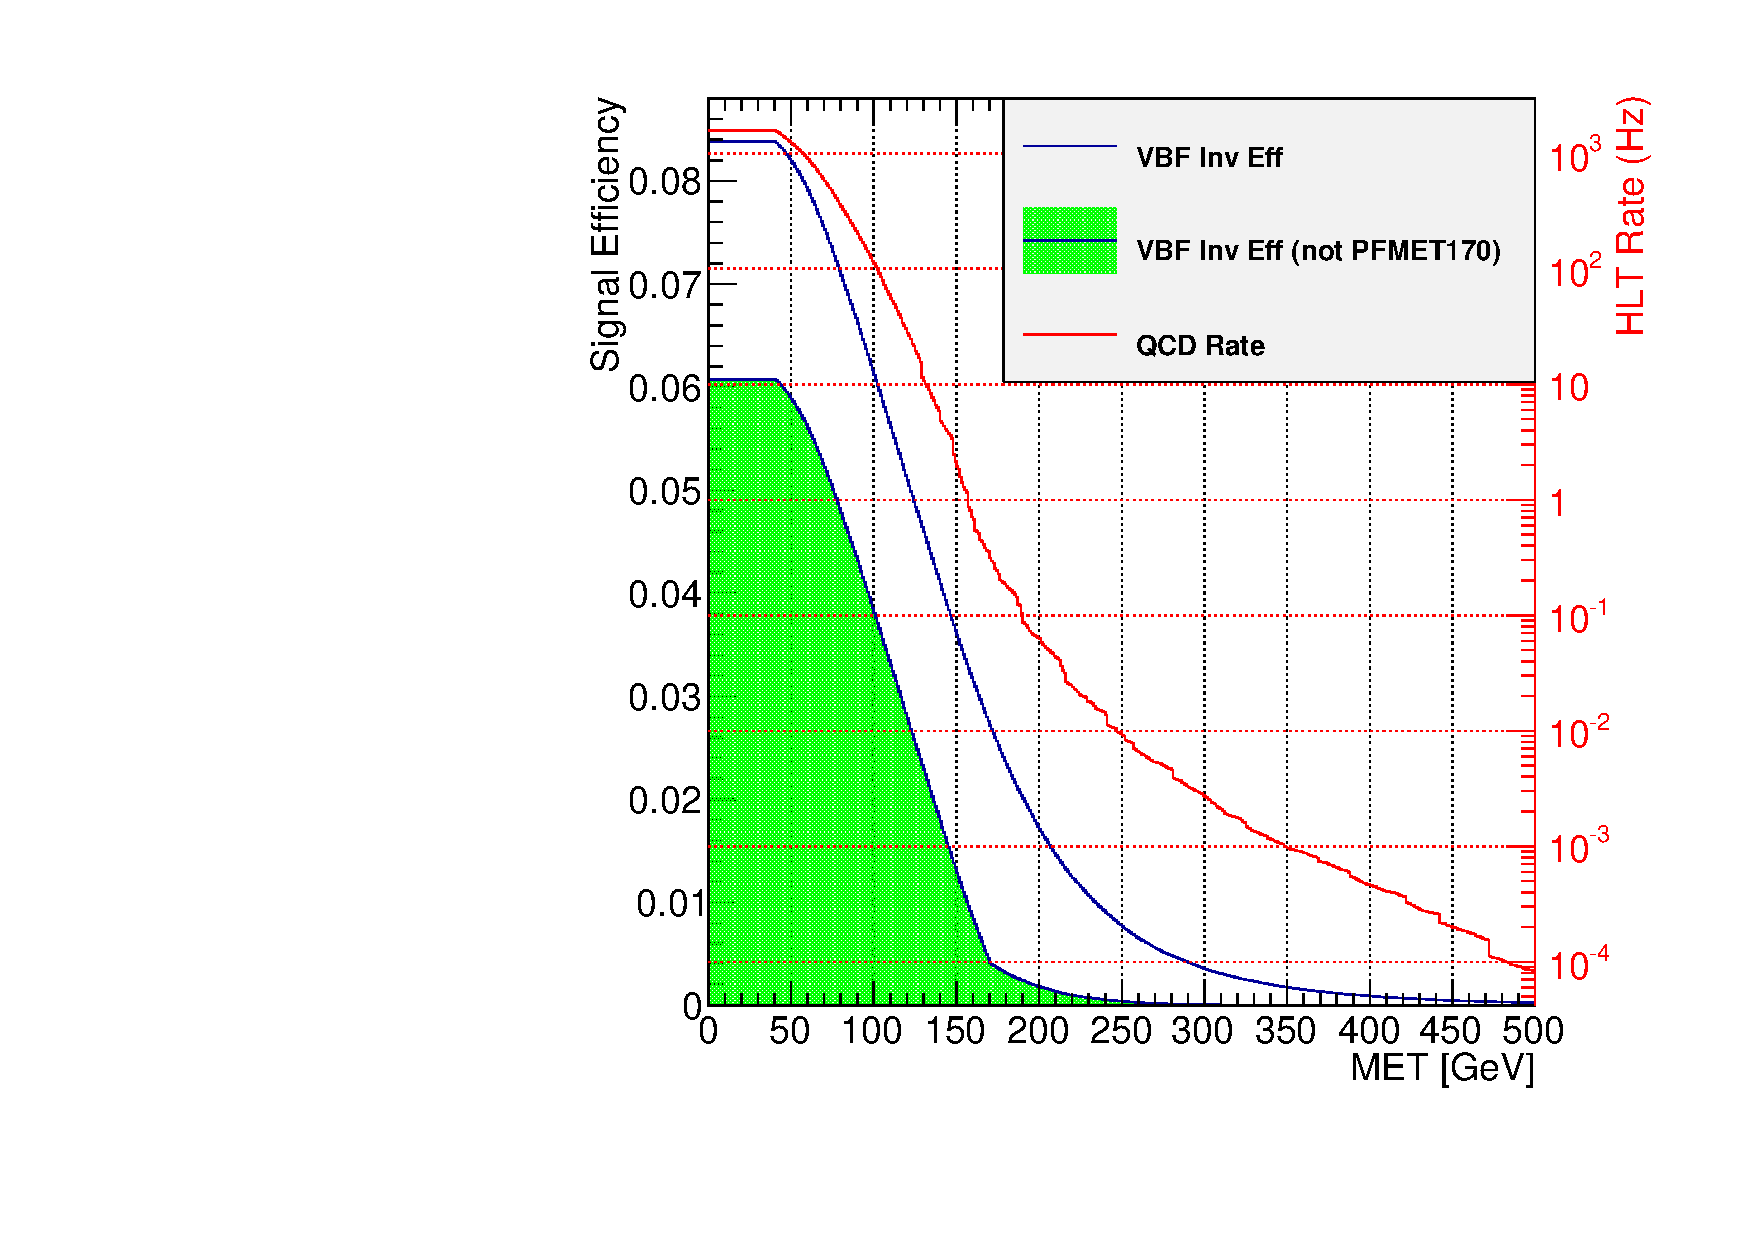
\includegraphics[width=0.45\linewidth]{Chapter08/TriggerStudies/HLT/Seed_DijetVBF30_DEta3p5_SingleJet96/HLT_DijetVBF40-40_DEta4p3_MJJ800.pdf}}\\
\caption{Plots showing the scan over \gls{HLT} \gls{PF} \gls{MET} for different algorithm base selection in the \textit{\gls{TSG} high luminosity scenario}. All \gls{HLT} algorithms are seeded by proposed \gls{L1T} algorithm selecting a dijet passing requirements \gls{VBF}, $\pt^{jets}>30\,\GeV$, and a single jet $\pt^{jets}>96\,\GeV$. Figure (a) base configuration requiring a dijet on opposite sides of the detector, $p_T^{jet_1},p_T^{jet_2}>90,40\,\GeV$, $\Delta\eta>4.1$ and $M_{jj}>500\,\GeV$ while figure (b) base configuration requiring a dijet on opposite sides of the detector, $p_T^{jet_1},p_T^{jet_2}>40,40\,\GeV$, $\Delta\eta>4.3$ and $M_{jj}>800\,\GeV$.}
\label{FIGURE:RunIITriggerStudies_HLT_Seed_L1TDijetSingleJet}
\end{figure}

The best additional signal efficiency algorithm optimized for this \gls{L1T} dijet plus single jet seed combined with the \gls{HLT} reference trigger records 11.26\% of the simulated signal process. This dedicated \gls{HLT} trigger, when compared with the proposed dedicated trigger for Run II, selects 19.8\% additional efficiency with an increase of 3.4\% in total signal efficiency. This trigger configuration most interesting feature is that it avoids completely the slow turn on of \gls{L1T} \gls{MET} which may allow lower offline \gls{MET} selection threshold.

%%%%%%%%%%%%%%%%%%%%%%%%%%%%%%%%%%%%%%%%%%%%%%%%%%%%%%%%%%%%%%%%%%%%%%%%%%%%%%%%%%%%%%%
%%% SUBSUBSECTION
%%%%%%%%%%%%%%%%%%%%%%%%%%%%%%%%%%%%%%%%%%%%%%%%%%%%%%%%%%%%%%%%%%%%%%%%%%%%%%%%%%%%%%%
\subsubsection{Systematics HLT trigger development}
\label{SECTION:RunIITriggerStudies_HLTAlgorithmDevelopment_SystematicsPath}

%Status: DONE (reviewed J.Pela x1)

One of the main systematics for the Run II analysis was the lack of statistics on the background control regions. In an attempt to solve this problem in Run II, it was seen as desirable to design a trigger algorithm with lower thresholds to study these regions. To allow the lowering of thresholds the trigger has to be prescaled. The target rate is for the low bandwidth scenario $0.1\,\hertz$ and $0.5\,\hertz$ for the high bandwidth scenario.

Considering the chosen dedicated \gls{HLT} trigger path presented in section \ref{SECTION:RunIITriggerStudies_HLTAlgorithmDevelopment_L1ETM70}, it was decided to make a background path with the lowest possible \gls{MET} requirement both at \gls{L1T} and \gls{HLT}. The \gls{L1T} algorithm chosen to seed this trigger path was \verb|L1_ETM50| which in the \gls{TSG} proposed menu is prescaled by 1000. The same automatic procedure used for the signal path studies was used here again. The maximum rate for this seed before any prescale applied was $500\,\hertz$ for the high bandwidth scenario of an \gls{HLT} output rate of $0.5\,\hertz$. The same base dijet configuration as the dedicated signal path was used, selecting events with a dijet on opposite sides of the detector passing requirements: $p_T^{jet_1},p_T^{jet_2}>40,40\,\GeV$, $\Delta\eta>3.5$ and $M_{jj}>600\,\GeV$. The obtained \gls{HLT} \gls{PF} \gls{MET} threshold was $80\,\GeV$ for an unprescaled rate of $505.75\,\hertz$. The final predicted rate for an \gls{HLT} prescale of 1 was $0.5\,\hertz$ and $0.1\,\hertz$ for an \gls{HLT} prescale of 5, as required by the study targets for each scenario. A plot of the scan over \gls{HLT} \gls{PF} \gls{MET} results from the optimization procedure can be found in figure \ref{FIGURE:RunIITriggerStudies_SystematicsPath}.

\begin{figure}[!htp]%
\centering
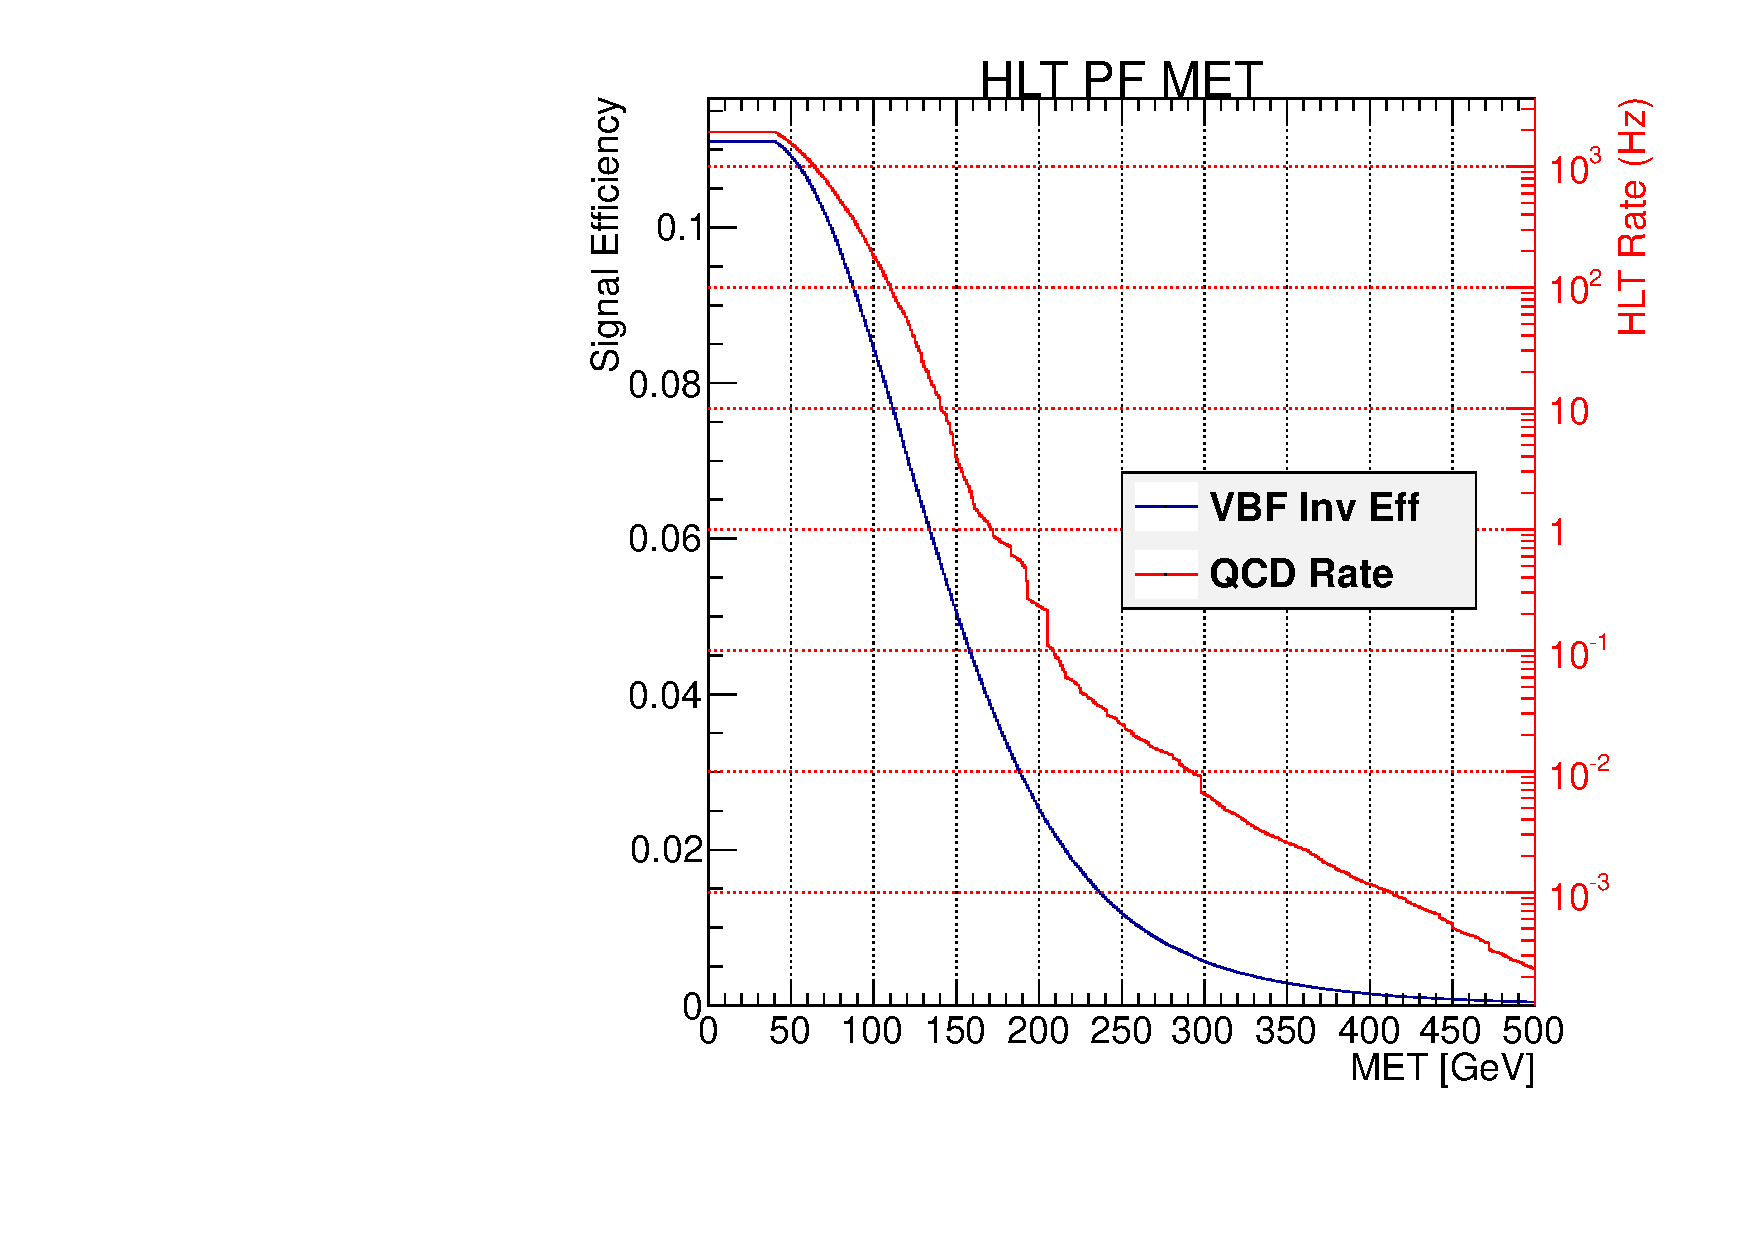
\includegraphics[width=0.55\linewidth]{Chapter08/TriggerStudies/HLT/Systematics/L1ETM50_HLT_DijetVBF40_DEta3p5_MJJ600.pdf}
\caption{Results of the automatic optimization of possible \gls{HLT} path for a maximum rate of $500\,\hertz$ for the \textit{\gls{TSG} high luminosity scenario}. The \gls{HLT} algorithm is seeded by L1\_ETM50. Figure shows the scan over \gls{HLT} \gls{PF} \gls{MET} for base configuration requiring a dijet on opposite sides of the detector, $p_T^{jet_1},p_T^{jet_2}>40,40$, $\Delta\eta>3.5$ and $M_{jj}>600\,\GeV$}
\label{FIGURE:RunIITriggerStudies_SystematicsPath}
\end{figure}

It was decided to propose to the \gls{TSG} the lowest rate background path with prescale 1000 at \gls{L1T} and 5 at \gls{HLT}. This proposal was accepted and a version of this trigger using \gls{PF} $\text{MET}_{no-\mu}$ was implemented and integrated into the standard \gls{CMS} trigger menu and was used to record data during the full 2015 Run II campaign.

%%%%%%%%%%%%%%%%%%%%%%%%%%%%%%%%%%%%%%%%%%%%%%%%%%%%%%%%%%%%%%%%%%%%%%%%%%%%%%%%%%%%%%%
%%% SUBSECTION
%%%%%%%%%%%%%%%%%%%%%%%%%%%%%%%%%%%%%%%%%%%%%%%%%%%%%%%%%%%%%%%%%%%%%%%%%%%%%%%%%%%%%%%
\subsection{Summary}
\label{SUBSECTION:RunIIPreparation_Summary}

%Status: DONE (reviewed J.Pela x1)

A complete study was preformed to define trigger conditions to record data during the \gls{LHC} Run II to be used by the \gls{VBF} Higgs to invisible analysis. Two \gls{HLT} triggers were proposed and accepted by the \gls{TSG} and included in the 2015 trigger menus. 

Considering a \gls{SM} \gls{VBF} Higgs to Invisible process with $m_H=125\,\GeV$, the signal is gathered by a combination of a general purpose trigger path, \verb|HLT_PFMET170_NoiseCleaned| and a dedicated trigger. The dedicated trigger is seeded by \verb|L1_ETM70| and selects events with at least one dijet on opposite sides of the detector passing requirements $p_T^{jets}>40\,\GeV$, $\Delta\eta>3.5$, $M_{jj}>600\,\GeV$ and \gls{PF} $\text{MET}_{no-\mu}>140\,\GeV$. Together these triggers collect 10.9\% of the simulated signal process where the dedicated path corresponds to an increase of signal collection efficiency of 15.8\% over the \gls{MET} only trigger. For the \textit{\gls{TSG} high luminosity scenario} the dedicated trigger is expected to have a pure rate under $5.0\,\hertz$. Turn on curves has been produced for this trigger with the full luminosity recorded during 2015, showing it is operating as expected.

A new background trigger path was developed, it is seeded by \verb|L1_ETM50| and selects events with at least one dijet on opposite sides of the detector passing requirements $p_T^{jets}>40\,\GeV$, $\Delta\eta>3.5$, and $M_{jj}>600\,\GeV$ and \gls{PF} $\text{MET}_{no-\mu}>80\,\GeV$. For the \textit{\gls{TSG} high luminosity scenario} an \gls{HLT} pure rate of $\approx 0.1\,\hertz$ is expected when applying a \gls{L1T} prescale of 1000 and 5 at \gls{HLT}.

Additionally, a study of new dedicated \gls{L1T} algorithms was preformed with the \gls{HLT} algorithms optimised for the highest additional rate when compared with the baseline triggers. It was demonstrated that the dedicated trigger additionally efficiency can be increased by 14.8\% by using a dedicated \gls{L1T} algorithm selecting events with a dijet plus \gls{MET} and by as much as 19.8\% when selecting events with a dijet plus a hard single jet. The latter would have the advantage of avoiding the slow turn-on the \gls{L1T} \gls{MET}. Both these options are being considered for the 2016 Run II campaign.

%%%%%%%%%%%%%%%%%%%%%%%%%%%%%%%%%%%%%%%%%%%%%%%%%%%%%%%%%%%%%%%%%%%%%%%%%%%%%%%%%%%%%%%
%%% SECTION
%%%%%%%%%%%%%%%%%%%%%%%%%%%%%%%%%%%%%%%%%%%%%%%%%%%%%%%%%%%%%%%%%%%%%%%%%%%%%%%%%%%%%%%
\section{Run II QCD Monte Carlo samples}
\label{SECTION:RunIIPreparation_RunIIQCDMonteCarloSamples}

%Status: DONE (reviewed J.Pela x1)

During the preparation of the Run I \gls{VBF} Higgs to invisible analysis, a set of \gls{QCD} samples with \gls{VBF}-like jets and real \gls{MET} were produced, described in section \ref{SECTION:PreparationParkedDataAnalysis_QCDVBFMET}. These samples enabled the understanding of the mechanisms that create real \gls{MET} in \gls{QCD} and how those could be mitigated. However, events with fake \gls{MET} were found to be the dominating type of QCD multi-jet events passing the analysis selection criteria. 

In the preparation for Run II, it was considered once again to be useful to have similar samples remade and possibly extended. It was identified that not only real \gls{MET} is significant but also fake \gls{MET} coming from detector mis-measurement. The \gls{QCD} background is currently the only background without any adequate representative \gls{MC} event sample. If such a sample could be produced, it could allow the analysis to evolve into a shape-based analysis or the use of machine learning techniques, since full description of the signal and backgrounds would be possible with simulations.

%%%%%%%%%%%%%%%%%%%%%%%%%%%%%%%%%%%%%%%%%%%%%%%%%%%%%%%%%%%%%%%%%%%%%%%%%%%%%%%%%%%%%%%
%%% SUBSECTION
%%%%%%%%%%%%%%%%%%%%%%%%%%%%%%%%%%%%%%%%%%%%%%%%%%%%%%%%%%%%%%%%%%%%%%%%%%%%%%%%%%%%%%%
\subsection{Goals and first attempt}
\label{SUBSECTION:RunIIPreparation_GoalsAndFirstAttempt}

%Status: DONE (reviewed J.Pela x1)

Building on the knowledge gained from the samples produced during Run I, we can define the goals for these new samples. Cuts at generator level involving \gls{MET} should be avoided in order to not filter out events where the \gls{MET} comes from mis-measurement. Variables that may bias the $\Delta\phi(jet-jet)$ distribution should also be avoided, as the Run I analysis uses inverted cuts in this variable to perform data-driven \gls{QCD} estimation. All cuts should be below the event selections used during Run I and, if possible, around or even below the Run II trigger conditions. The sample to be simulated should be equivalent to at least $1\,\femto\barn^{-1}$ of data but of a size comparable with the current official \gls{QCD} Inclusive sample. This last requirement is to ensure that the computing resources necessary for making such sample do not go above those currently used to produce similar purpose samples. 

The first attempt to produce a proposal for the production of this \gls{QCD} \gls{VBF}-like sample was based on filtering events produced by \textsc{PYTHIA 8}. This filtering was done by first clustering the generator particles in anti-$k_T$ jets with $R=0.4$, where muons were ignored. Only events with at least one dijet with \gls{VBF} characteristics would be kept. Unfortunately, this approach leads to a very large number of event being generated (hard scattering and hadronization) and clustered, only to be discarded. The computing time was considered too large to be feasible considering the physics case by the \gls{CMS} team responsible for official sample production. However, it was recommended to take a different approach by using a \gls{ME} generator, like \textsc{MADGRAPH}, and to cut at the parton level, before any hadronization or clustering. After this initial event selection, a second layer of cuts could be applied after hadronization to ensure the actual outgoing jets would pass offline selection criteria. Furthermore, using a \gls{ME} generator should provide a more accurate description of multi-jet events, while the two-step approach should allow a significant reduction of the necessary computing time. 

%%%%%%%%%%%%%%%%%%%%%%%%%%%%%%%%%%%%%%%%%%%%%%%%%%%%%%%%%%%%%%%%%%%%%%%%%%%%%%%%%%%%%%%
%%% SUBSECTION
%%%%%%%%%%%%%%%%%%%%%%%%%%%%%%%%%%%%%%%%%%%%%%%%%%%%%%%%%%%%%%%%%%%%%%%%%%%%%%%%%%%%%%%
\subsection{\textsc{MADGRAPH} parton level simulation}
\label{SUBSECTION:RunIIPreparation_MadGraphPartonLevelSimulation}

%Status: DONE (reviewed J.Pela x1)

The \textsc{MADGRAPH} event generator was selected to produce the parton level simulation. With this generator it is possible to simulate events from the interaction of two proton partons and to obtain a final state with any number of partons. Each additional parton on the final state comes at the cost of an exponential increase of the possible diagrams, which in turn means more time is necessary to create events. It was chosen to only produce final states with 2, 3 and 4 outgoing partons. This generator has been used to create similar \gls{QCD} samples used by some \gls{CMS} \gls{SUSY} analyses. 

The outgoing partons are defined to be a gluon or a quark (u, d, c, s or b). We do not allow diagrams with top quarks as they do not hadronize and lead to event topologies which are already accounted by other \gls{MC} samples. The outgoing partons are the seeds of our final state jets. 

A custom parton level filter was implemented inside the \textsc{MADGRAPH} code to select events with \gls{VBF} characteristics. To pass the filter, the event must have at least one outgoing di-parton with invariant mass of $800\,\GeV$, where both parton are inside the detector volume with $|\eta|<5.0$ and have $p_{T}>30\,\GeV$. The distributions of these variables for events passing this cuts can be found in figure \ref{FIGURE:RunIIPreparation_PassPartonFilterDistributions}.

\begin{figure}[!htp]%
\centering
\subfloat[][]{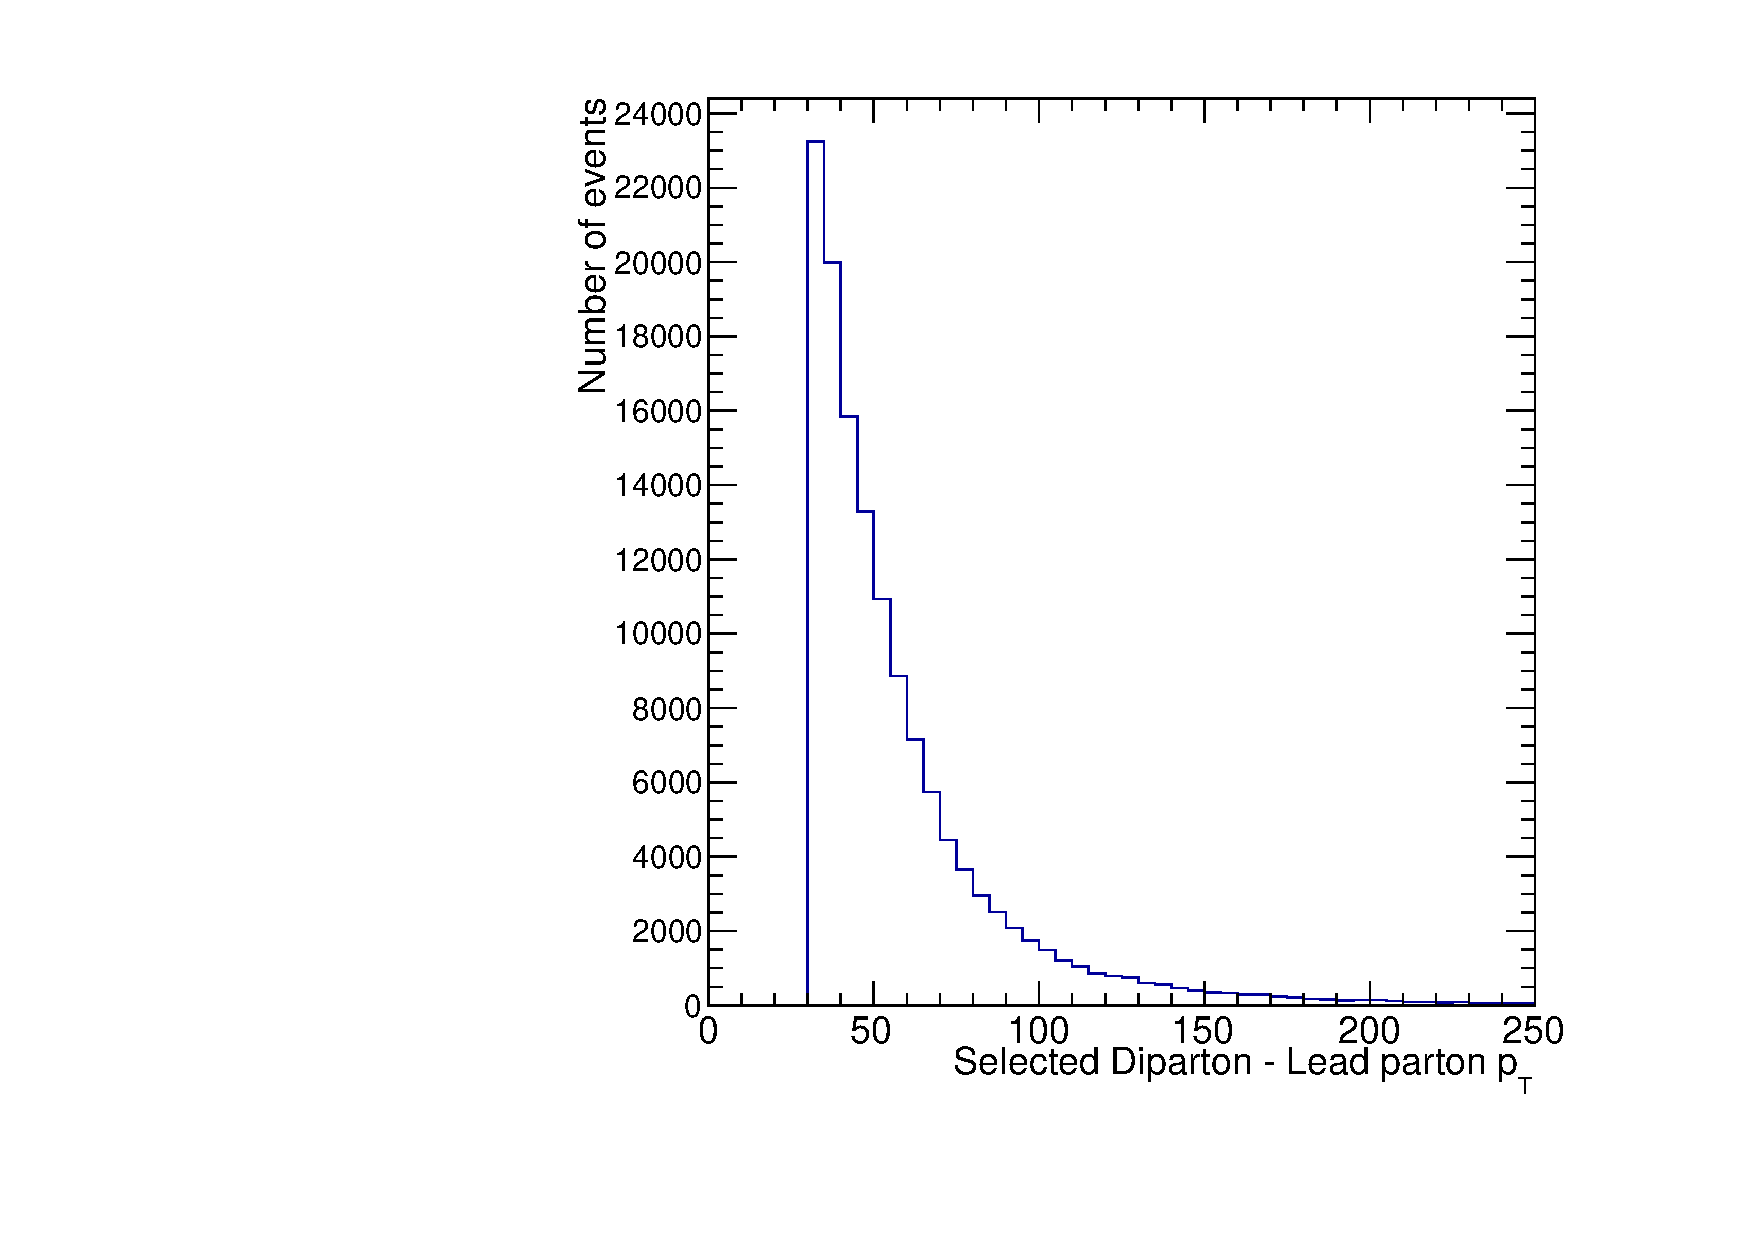
\includegraphics[width=0.40\linewidth]{Chapter08/QCDVBFSamples/PartonFilter/Images/SelDiParton_Parton1_Pt.pdf}}\qquad
\subfloat[][]{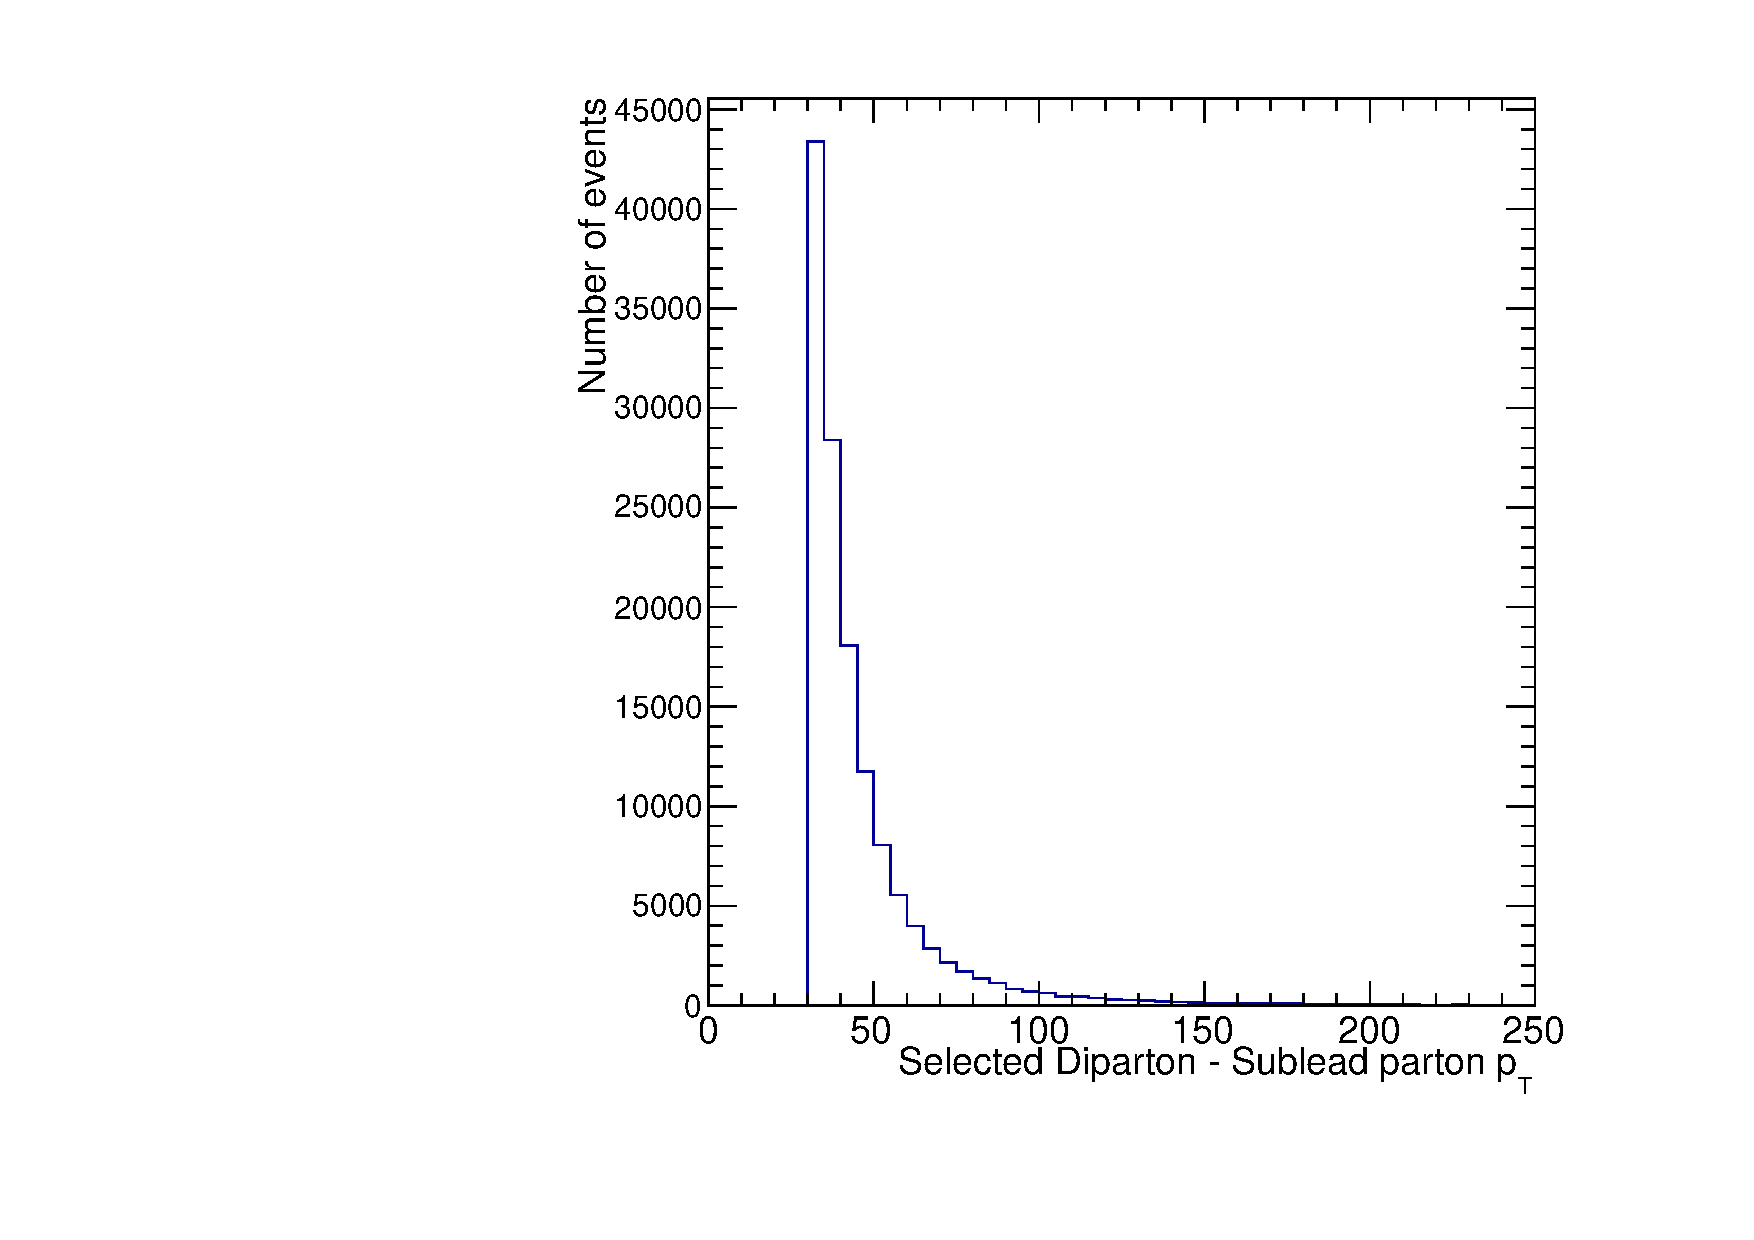
\includegraphics[width=0.40\linewidth]{Chapter08/QCDVBFSamples/PartonFilter/Images/SelDiParton_Parton2_Pt.pdf}}\\
\subfloat[][]{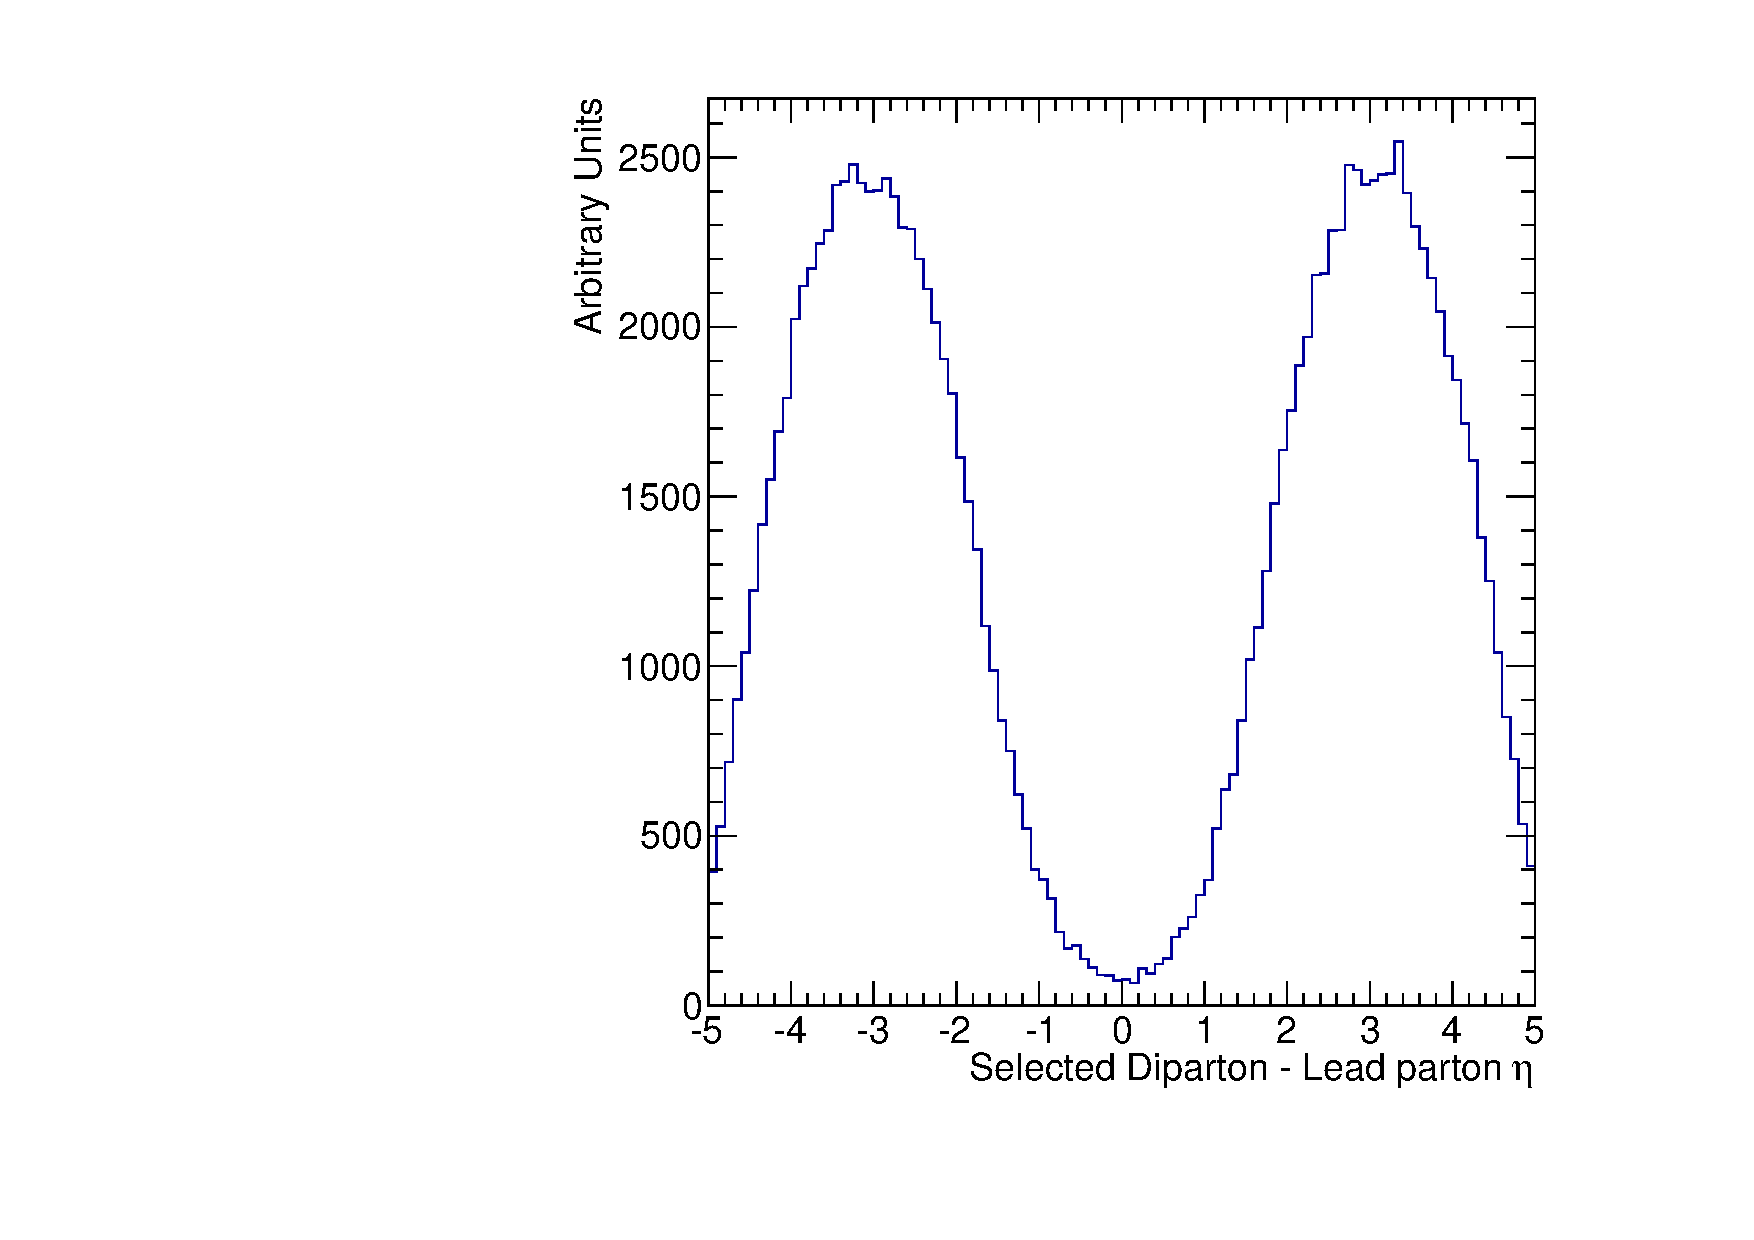
\includegraphics[width=0.40\linewidth]{Chapter08/QCDVBFSamples/PartonFilter/Images/SelDiParton_Parton1_Eta.pdf}}\qquad
\subfloat[][]{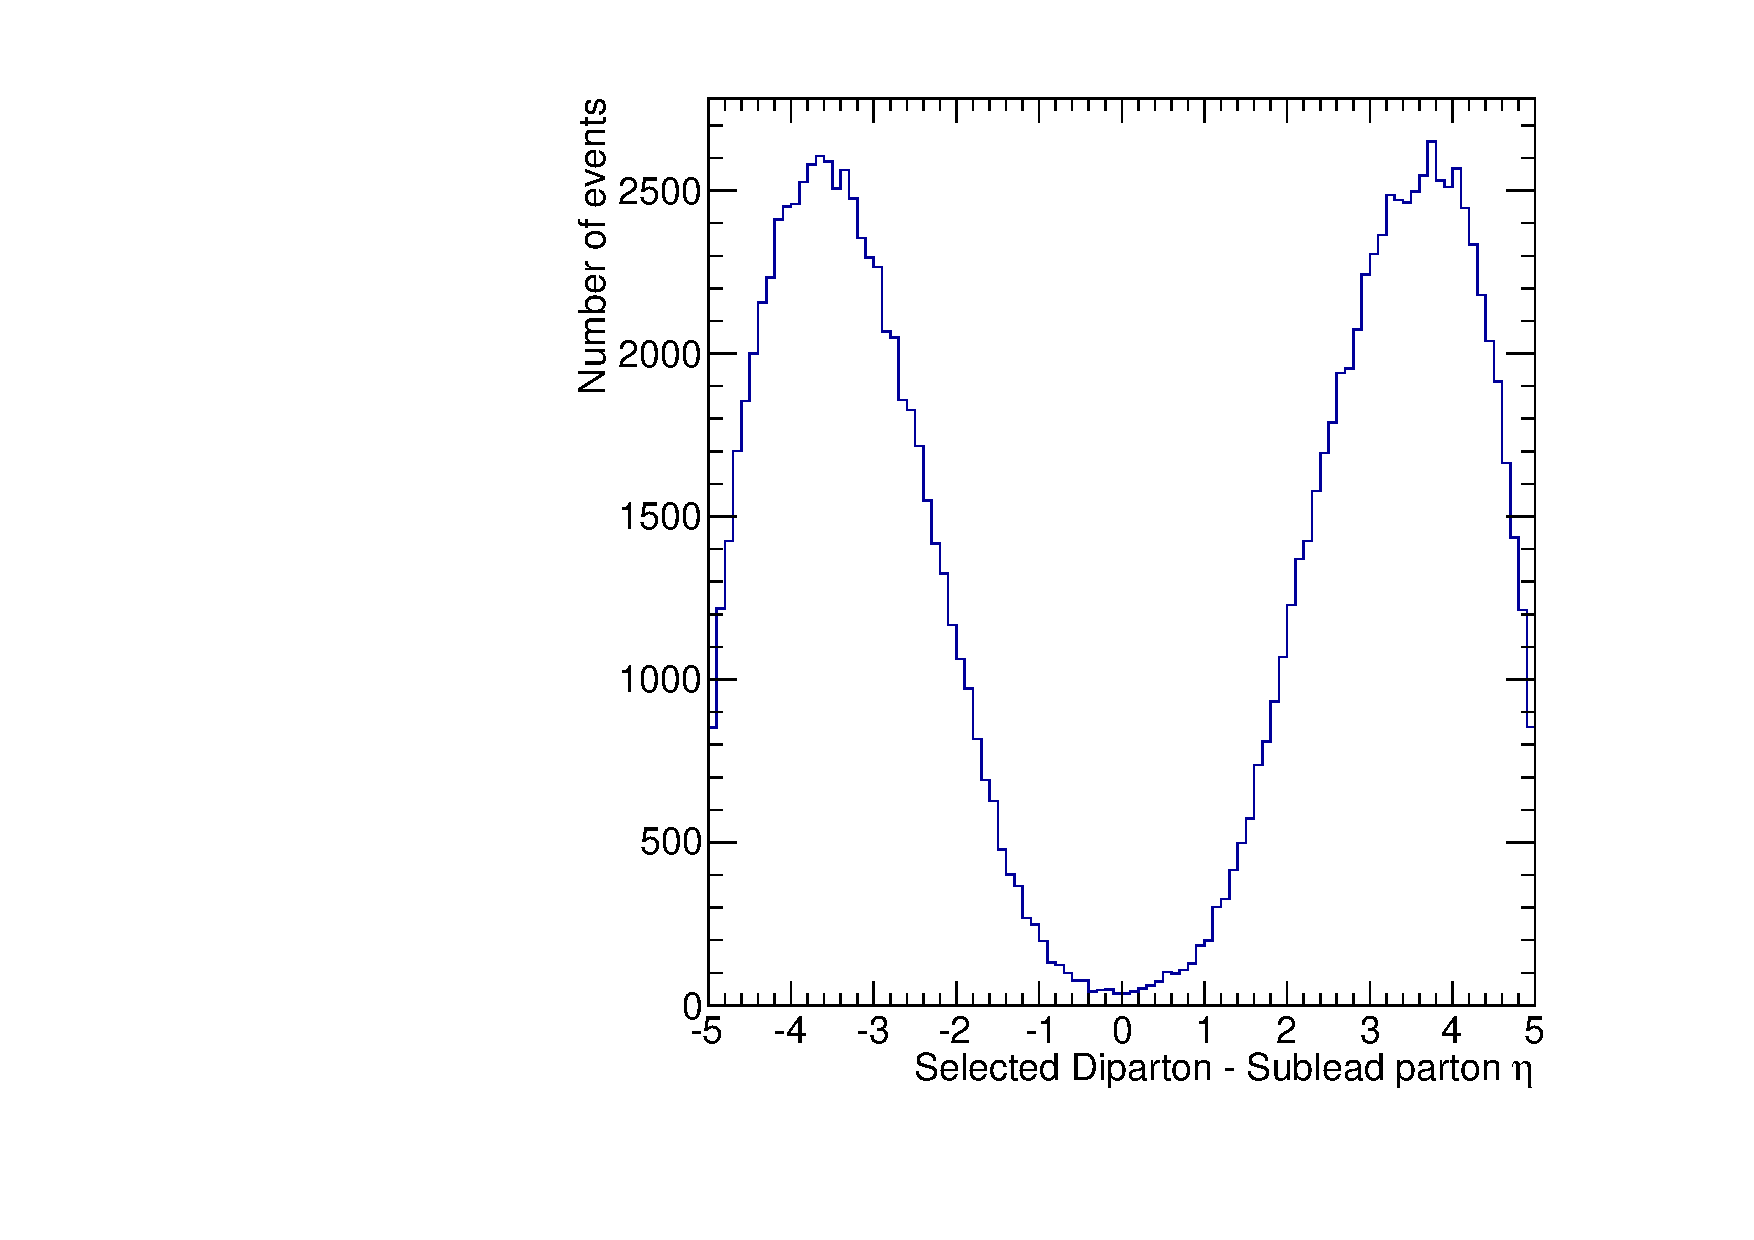
\includegraphics[width=0.40\linewidth]{Chapter08/QCDVBFSamples/PartonFilter/Images/SelDiParton_Parton2_Eta.pdf}}\\
% \subfloat[][]{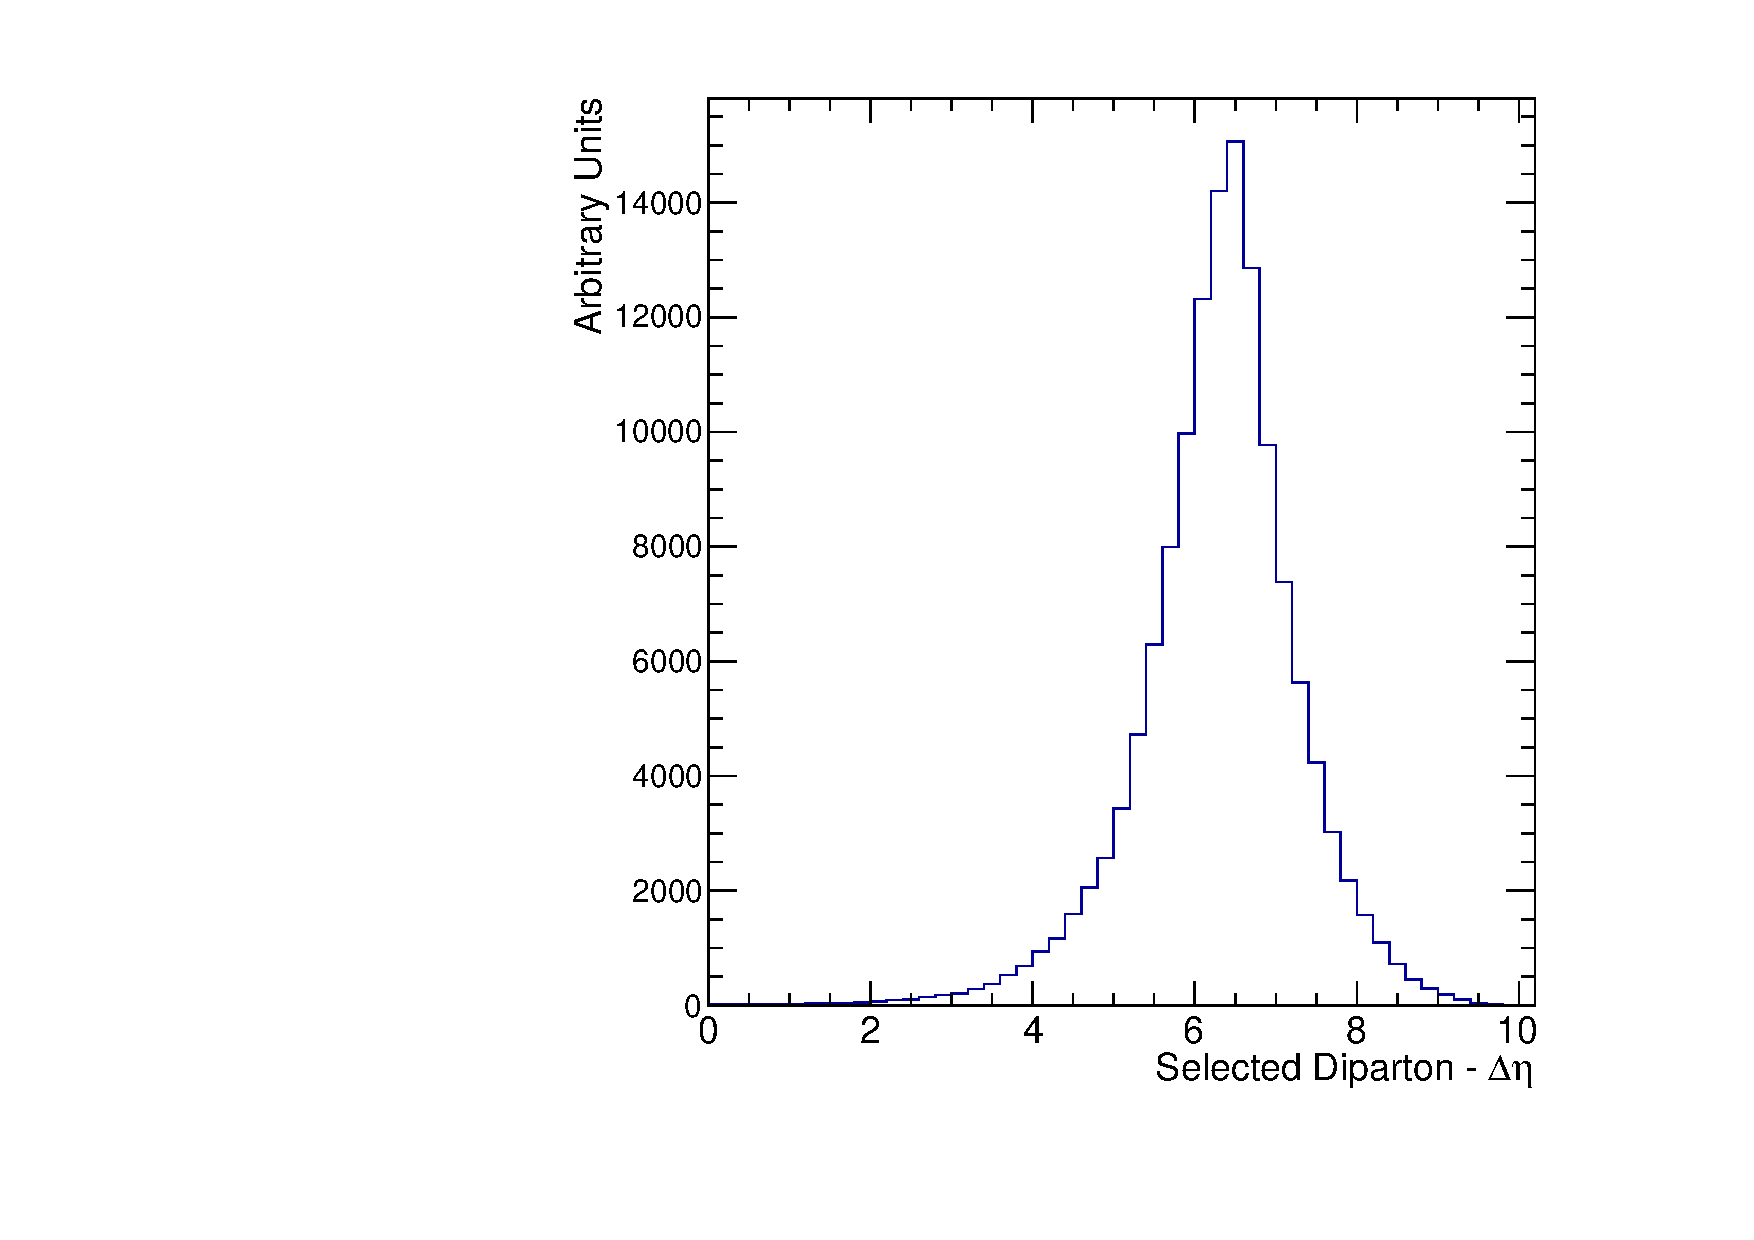
\includegraphics[width=0.45\linewidth]{Chapter08/QCDVBFSamples/PartonFilter/Images/SelDiParton_DEta.pdf}}\qquad
% \subfloat[][]{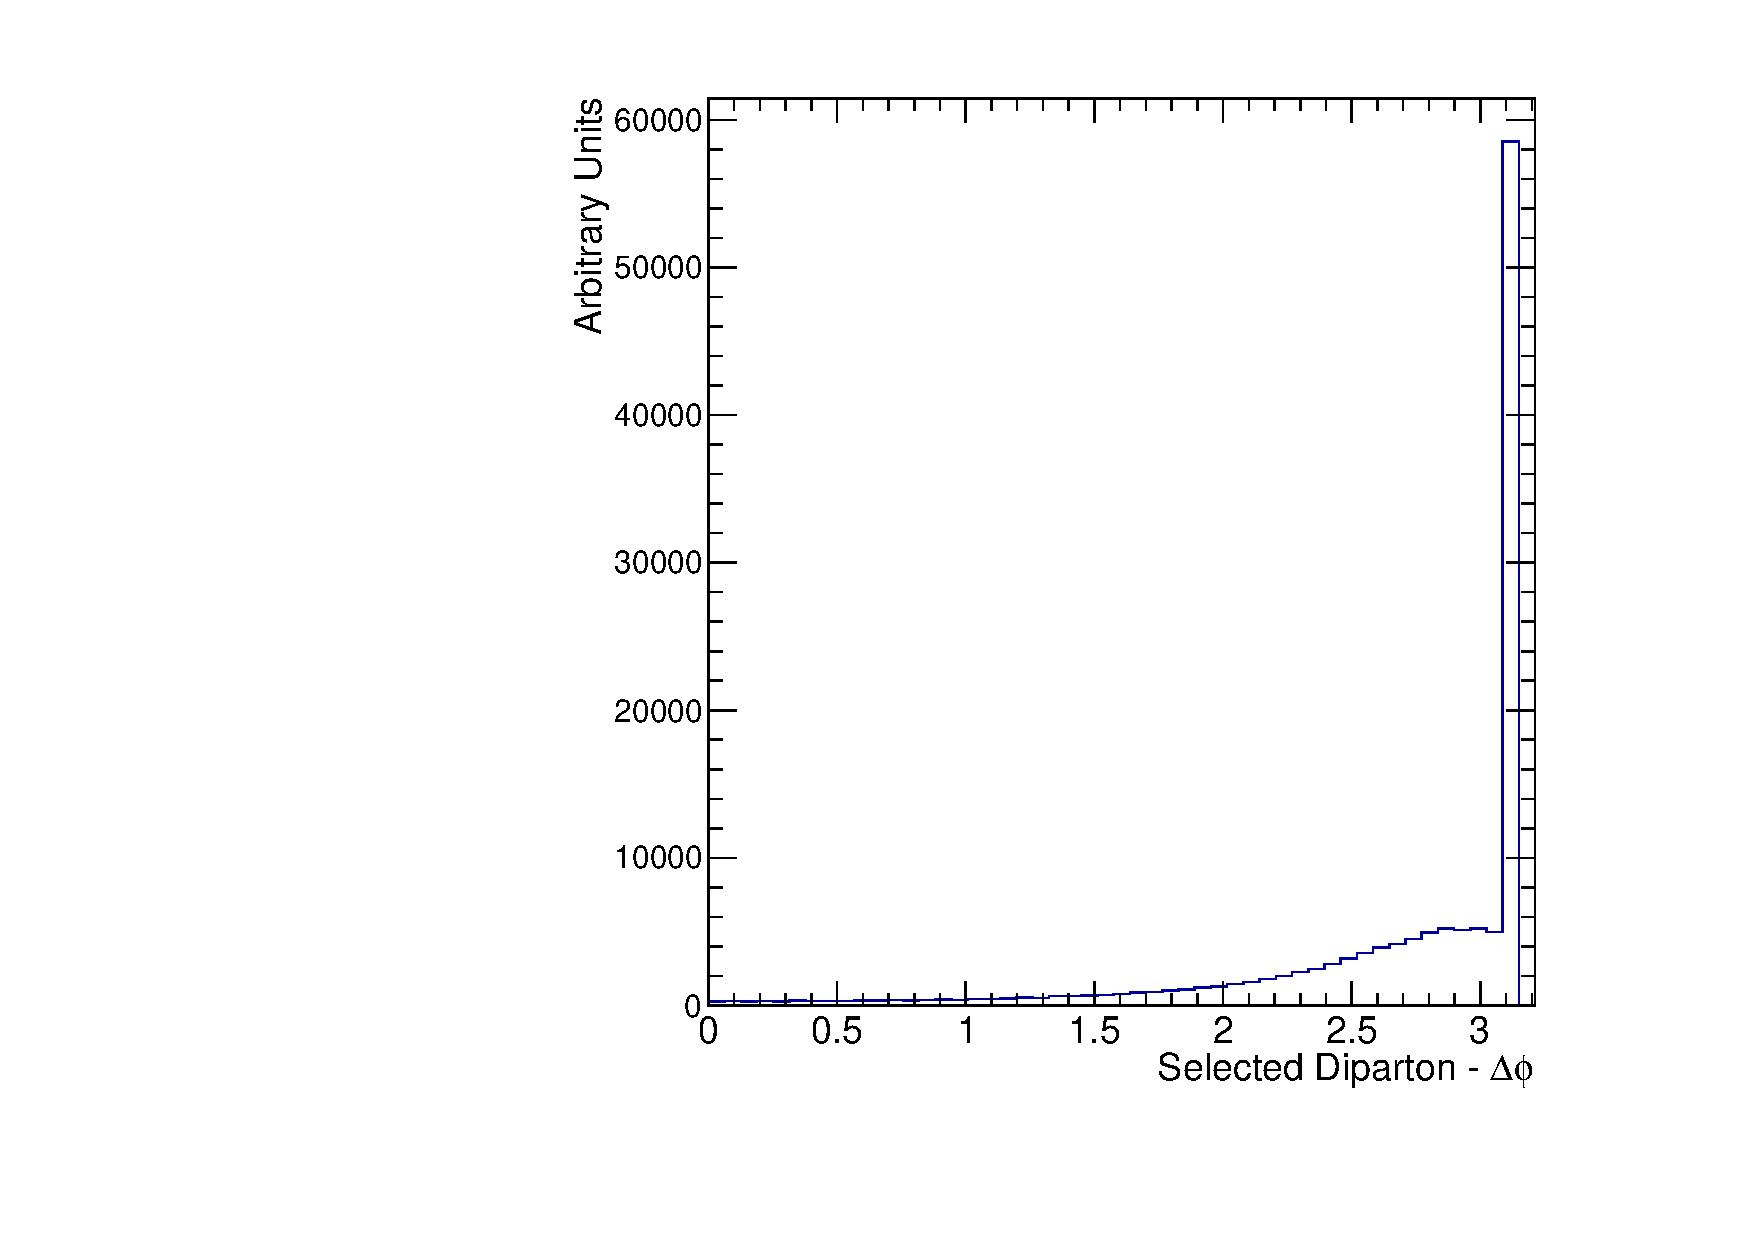
\includegraphics[width=0.45\linewidth]{Chapter08/QCDVBFSamples/PartonFilter/Images/SelDiParton_DPhi.pdf}}\\
\subfloat[][]{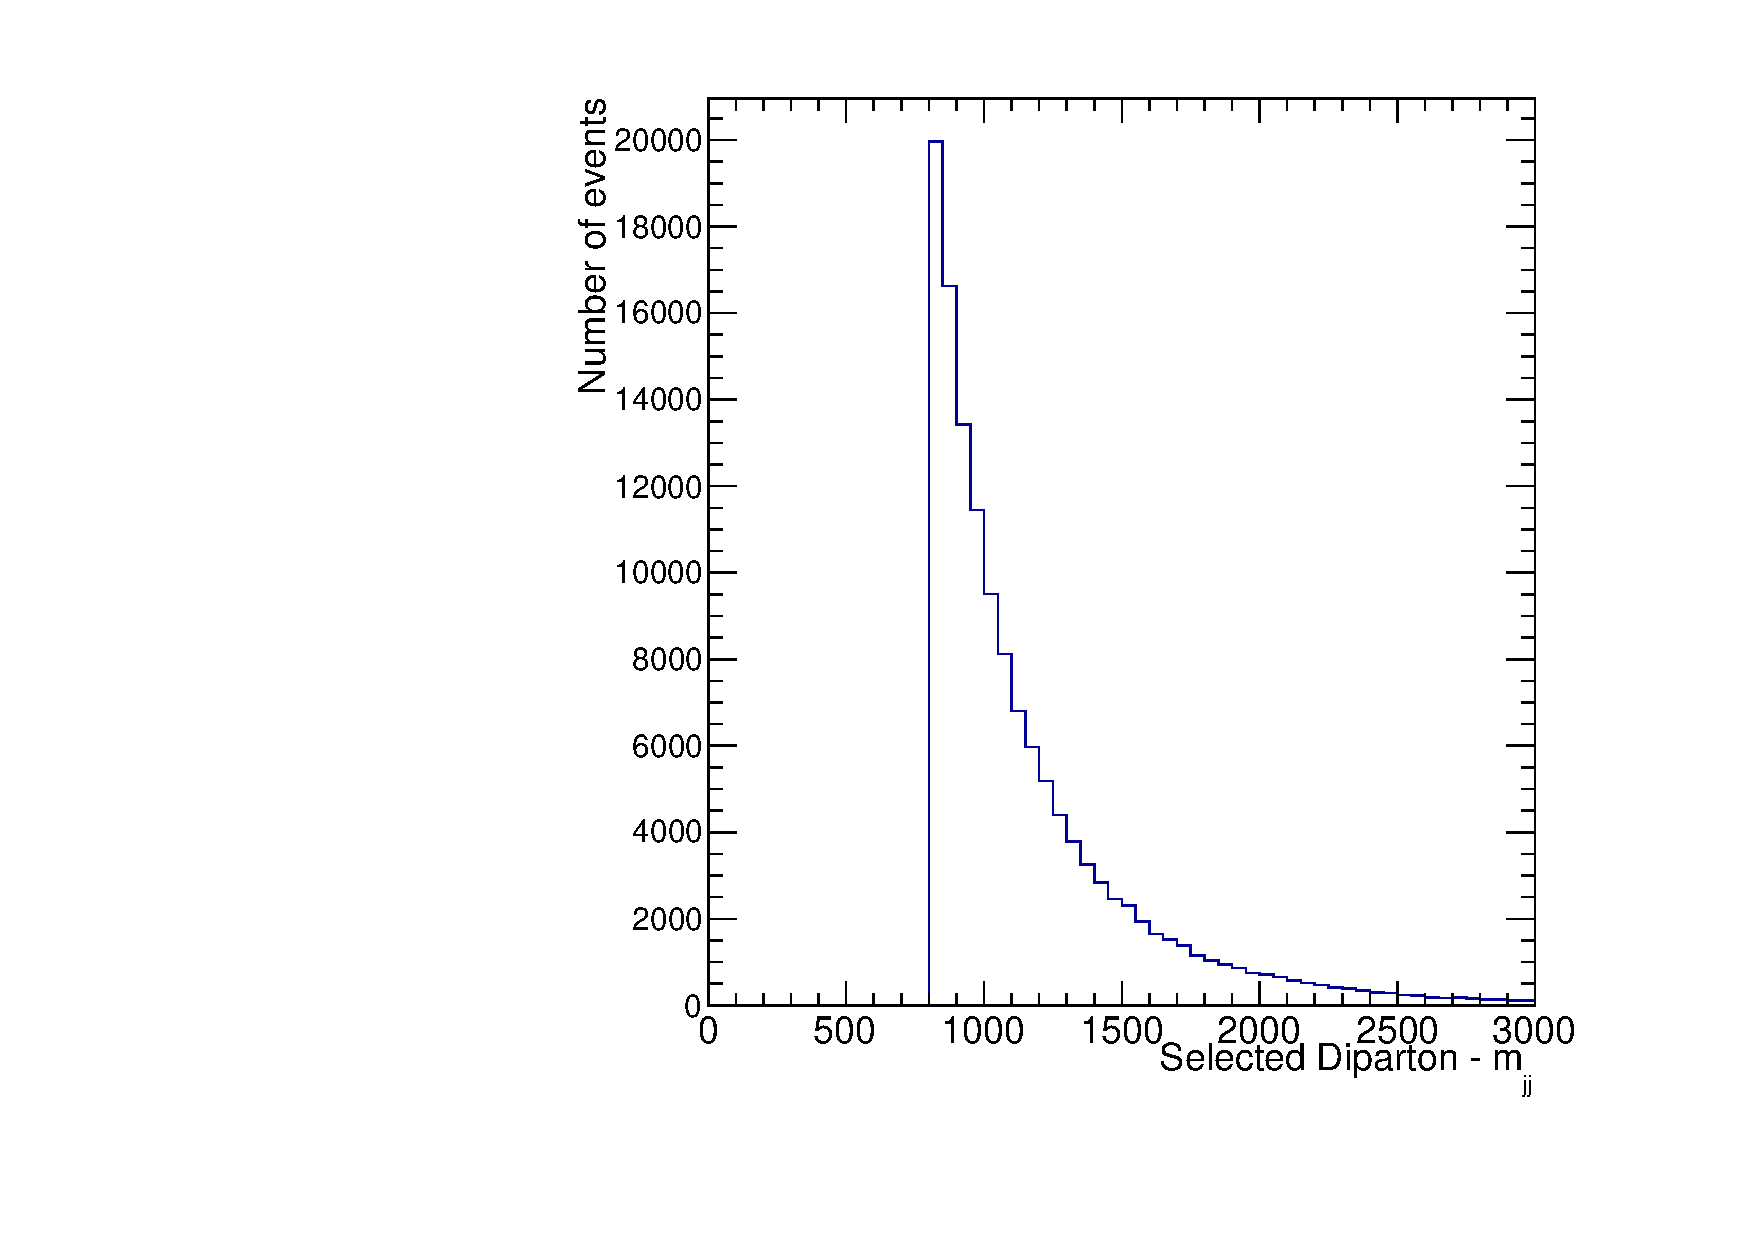
\includegraphics[width=0.40\linewidth]{Chapter08/QCDVBFSamples/PartonFilter/Images/SelDiParton_Mjj.pdf}}\\
\caption[Key variables of events passing the parton level filter]{Parton \pt, $\eta$ and di-parton $m_jj$ distributions for the leading di-parton passing cuts: parton $p_{T}>30\,\GeV$ and $|\eta|<5.0$, di-parton $M_{jj}>800\,\GeV$.}
\label{FIGURE:RunIIPreparation_PassPartonFilterDistributions}
\end{figure}

The estimated cross section for these processes and selection is $(1.029 \pm 0.002) \times 10^7 \,\pico\barn$ and we request the production of $1.2 \times 10^{10}$ events. That corresponds to just over $1.1\,\femto\barn^{-1}$ of equivalent integrated luminosity. 

%%%%%%%%%%%%%%%%%%%%%%%%%%%%%%%%%%%%%%%%%%%%%%%%%%%%%%%%%%%%%%%%%%%%%%%%%%%%%%%%%%%%%%%
%%% SUBSECTION
%%%%%%%%%%%%%%%%%%%%%%%%%%%%%%%%%%%%%%%%%%%%%%%%%%%%%%%%%%%%%%%%%%%%%%%%%%%%%%%%%%%%%%%
\subsection{Hadronization with \textsc{PYTHIA 8}}
\label{SUBSECTION:RunIIPreparation_HadronizationWithPythia8}

%Status: DONE (reviewed J.Pela x1)

The parton level events that have passed the initial filter are then hadronized. Similarly to other samples produced in \gls{CMS}, \textsc{PYTHIA 8} was chosen for this. As described in section \ref{SECTION:EventReconstructionAndSimulation_MonteCarloSimulation}, when using a \gls{ME} generator with a shower generator we need to filter the overlapping phase-space. As recommened by the \gls{CMS} generator group we used the MLM scheme~\cite{ARTICLE:MLMScheme} with the same parameters used for the production of previous official samples. The results of the hadronization process are summarized in table \ref{TABLE:RunIIPreparation_Pythia8HadronizationResults}.

\begin{table}[!htp]
\centering

\resizebox{1.0\textwidth}{!}{
\begin{tabular}{|c|c|c|c|c|c|}
\hline
                          & \multicolumn{3}{c|}{Events}      & \multicolumn{2}{c|}{Cross Section [pb]}                \\
\hline
Process                   &  Tried  & Passed & accepted [\%]  & Before                    & After                     \\
\hline\hline 
$p p \rightarrow j j$     &  231789 &  54291 & $23.4 \pm 1.01$ & $1.675 \times 10^6 \pm 4.536 \times 10^3$ & $3.924 \times 10^5 \pm 1.817 \times 10^3$ \\
$p p \rightarrow j j j$   &  502287 &  36250 & $ 7.2 \pm 0.03$ & $3.622 \times 10^6 \pm 9.809 \times 10^3$ & $2.614 \times 10^5 \pm 1.500 \times 10^3$ \\
$p p \rightarrow j j j j$ &  692600 &  44299 & $ 6.4 \pm 0.03$ & $4.972 \times 10^6 \pm 1.346 \times 10^4$ & $3.180 \times 10^5 \pm 1.697 \times 10^3$ \\
\hline\hline
Total                     & 1426676 & 134840 & $9.45 \pm 0.03$ & $1.027 \times 10^7 \pm 1.727 \times 10^4$ & $9.718 \times 10^5 \pm 2.903 \times 10^3$ \\
\hline
\end{tabular}
}
\caption{Summary of the results of the Hadronization with Pythia 8 of 1.4M MadGraph events passing the parton level filter.}
\label{TABLE:RunIIPreparation_Pythia8HadronizationResults}
\end{table}

% --------------------------------------------------------------------------------------------------------------------------------------------------------------------------
% Process and cross-section statistics
% --------------------------------------------------------------------------------------------------------------------------------------------------------------------------
% Process         xsec_before [pb]                passed  nposw   nnegw   tried   nposw   nnegw   xsec_match [pb]                 accepted [%]     event_eff [%]
% 0               1.675e+06 +/- 4.536e+03         54291   54291   0       231789  231789  0       3.924e+05 +/- 1.817e+03         23.4 +/- 0.1    23.4 +/- 0.1       1.0052431
% 1               3.622e+06 +/- 9.809e+03         36250   36250   0       502287  502287  0       2.614e+05 +/- 1.500e+03          7.2 +/- 0.0     7.2 +/- 0.0       0.037905486
% 2               4.972e+06 +/- 1.346e+04         44299   44299   0       692600  692600  0       3.180e+05 +/- 1.697e+03          6.4 +/- 0.0     6.4 +/- 0.0       0.030388865
% --------------------------------------------------------------------------------------------------------------------------------------------------------------------------
% Total           1.027e+07 +/- 1.727e+04         134840  134840  0       1426676 1426676 0       9.718e+05 +/- 2.903e+03          9.5 +/- 0.0     9.5 +/- 0.0
% --------------------------------------------------------------------------------------------------------------------------------------------------------------------------


The efficiency of the post-hadronization event matching has been estimated to be $9.45\% \pm 0.03\%$, leading to a sample cross section of $(9.718 \pm 0.03) \times 10^5\,\pico\barn$. The lower matching efficiency in the 3 and 4 jets final states is due to the absence of a restriction on minimum jet \pt on any additional jets to the dijet passing the parton level cuts. These additional generator jets, if low enough in energy, will hardlybe picked up by the clustering algorithm and therefore cannot be matched to their seed parton.

%%%%%%%%%%%%%%%%%%%%%%%%%%%%%%%%%%%%%%%%%%%%%%%%%%%%%%%%%%%%%%%%%%%%%%%%%%%%%%%%%%%%%%%
%%% SUBSECTION
%%%%%%%%%%%%%%%%%%%%%%%%%%%%%%%%%%%%%%%%%%%%%%%%%%%%%%%%%%%%%%%%%%%%%%%%%%%%%%%%%%%%%%%
\subsection{Generator level cuts}
\label{SUBSECTION:RunIIPreparation_GeneratorLevelCuts}

%Status: DONE (reviewed J.Pela x1)

After hadronization we cluster the outgoing stable particles with the anti-$k_T$ algorithm with $R=0.4$ while ignoring muons. The reason for ignoring muons is that \gls{CMS} muon detector coverage only goes up to $|\eta|<2.4$, so all muons outside this region will not be seen by the experiment and therefore will not be clustered into jets. Most of our signal like events will have at least one jet in the region $|\eta|>2.4$. For the jets inside the muon systems acceptance, the jet \pt will be underestimated when a muon is present, but this effect was assumed to be small.

We start by making an initial selection of the events with at least one generator level dijet passing $\Delta\eta > 3.0$, $M_{jj} > 1000\,\GeV$ where both jets pass $\pt > 40\,\GeV$ and $|\eta|<4.8$, this selection is thresholds are below all offline requirements of the parked data analysis. The events passing this selection are split into two sub-samples. Sub-sample A has events where the selected dijet passes $\Delta\phi \leq 2.15$ and sub-sample B where at least one dijet passes all initial conditions and an inverted $\Delta\phi$ requirement. Plots over all the relevant variable before the $\Delta\phi$ requirement and for the leading dijet passing the cuts can be found in figure \ref{FIGURE:RunIIPreparation_PassGeneratorFilterDistributions1} and \ref{FIGURE:RunIIPreparation_PassGeneratorFilterDistributions2}.

\begin{figure}[!htp]%
\centering
\subfloat[][]{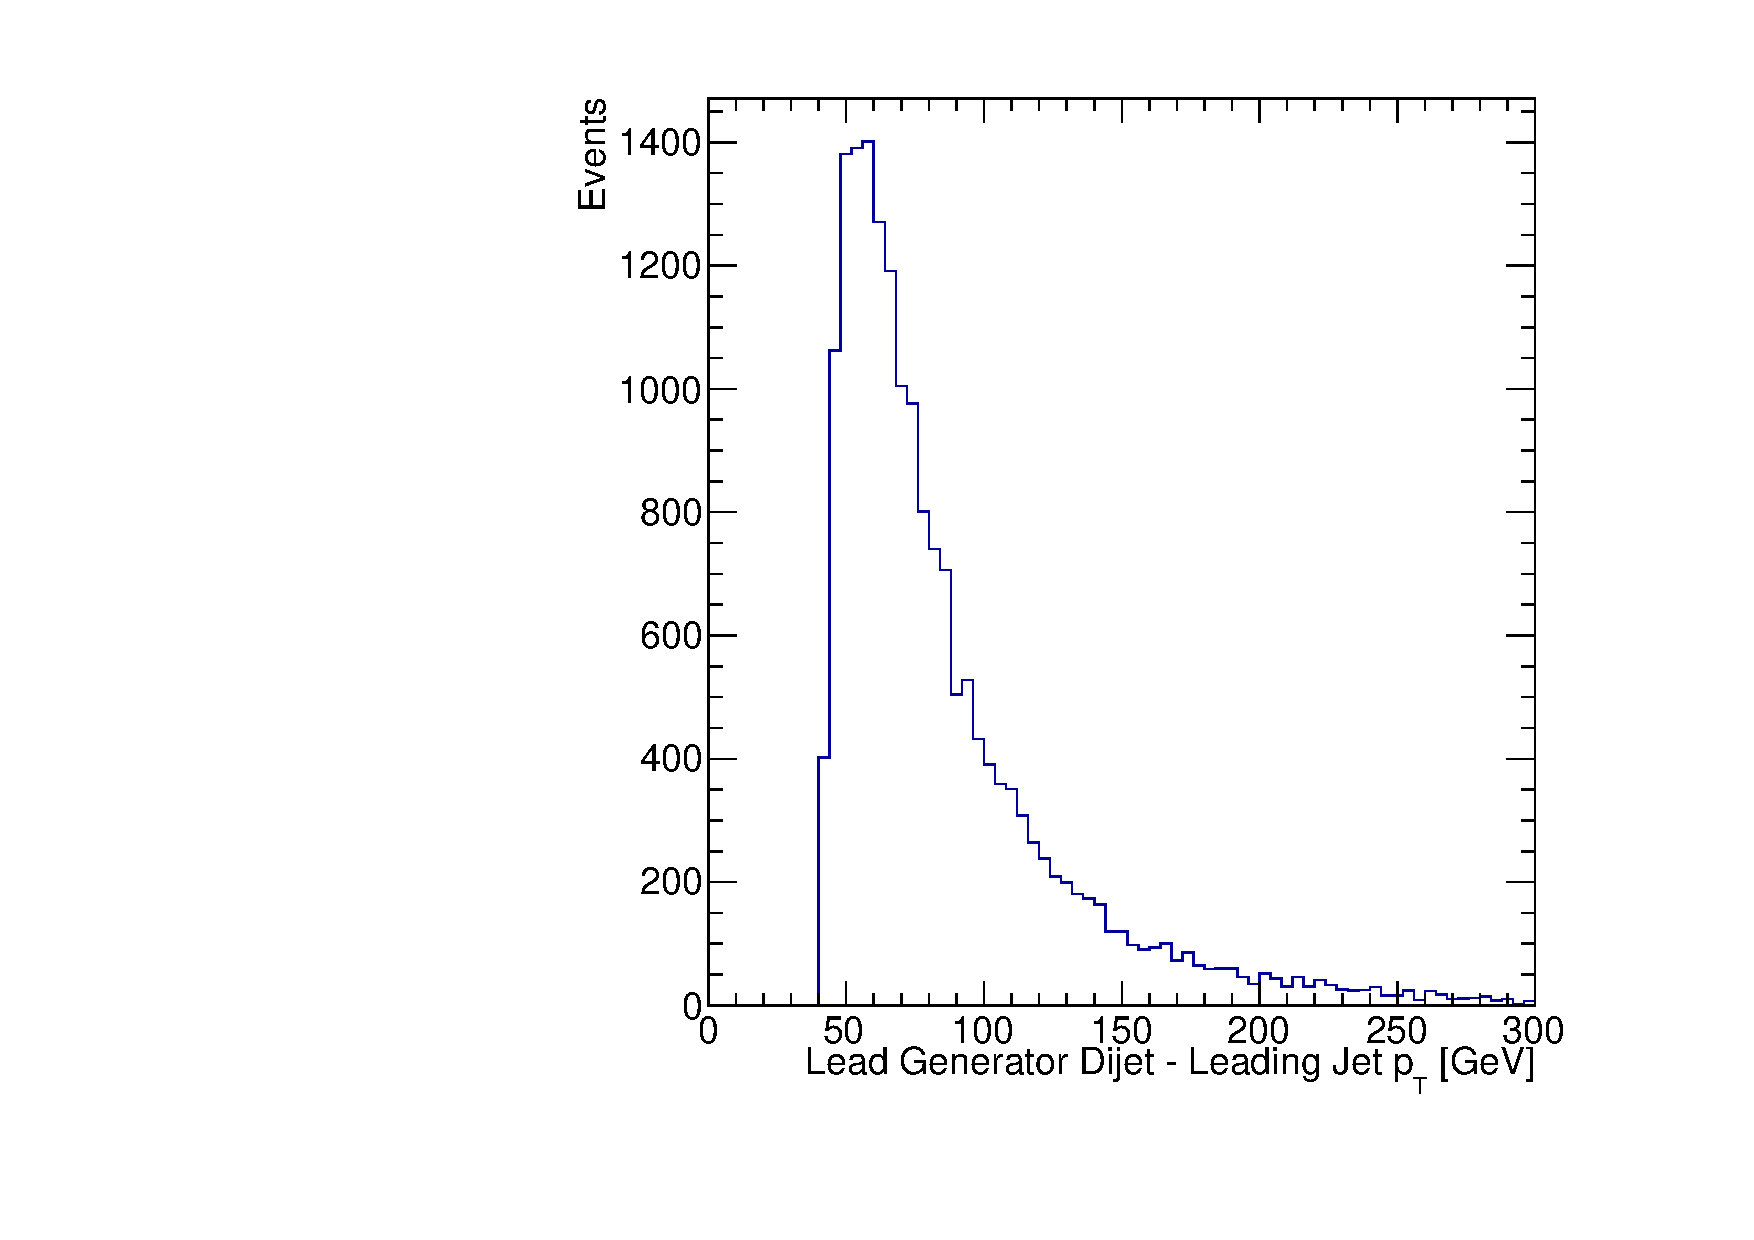
\includegraphics[width=0.40\linewidth]{Chapter08/QCDVBFSamples/GeneratorFilter/Pt40_Eta4p8_DEta3p0_Mjj1000/Images/LeadDijet_Jet0_Pt.pdf}}\qquad
\subfloat[][]{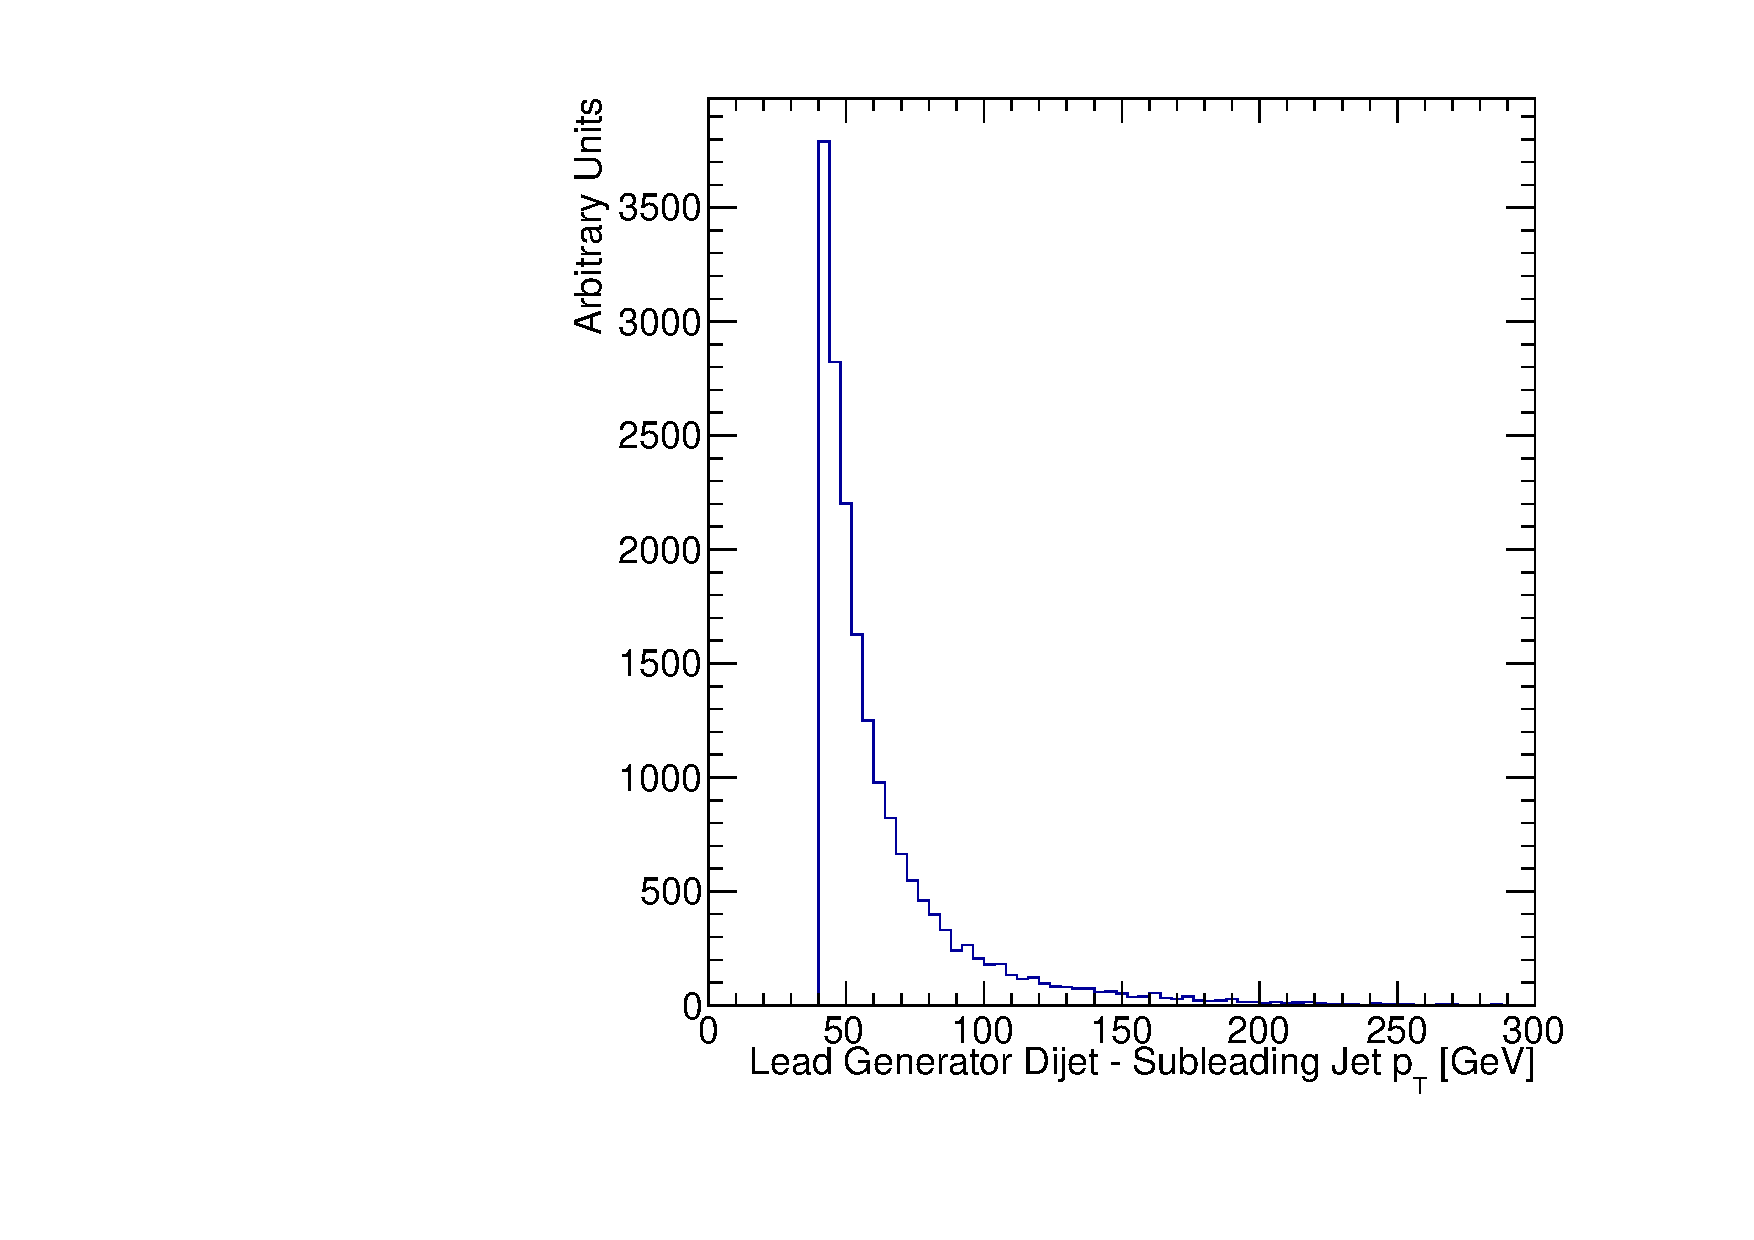
\includegraphics[width=0.40\linewidth]{Chapter08/QCDVBFSamples/GeneratorFilter/Pt40_Eta4p8_DEta3p0_Mjj1000/Images/LeadDijet_Jet1_Pt.pdf}}\\
\subfloat[][]{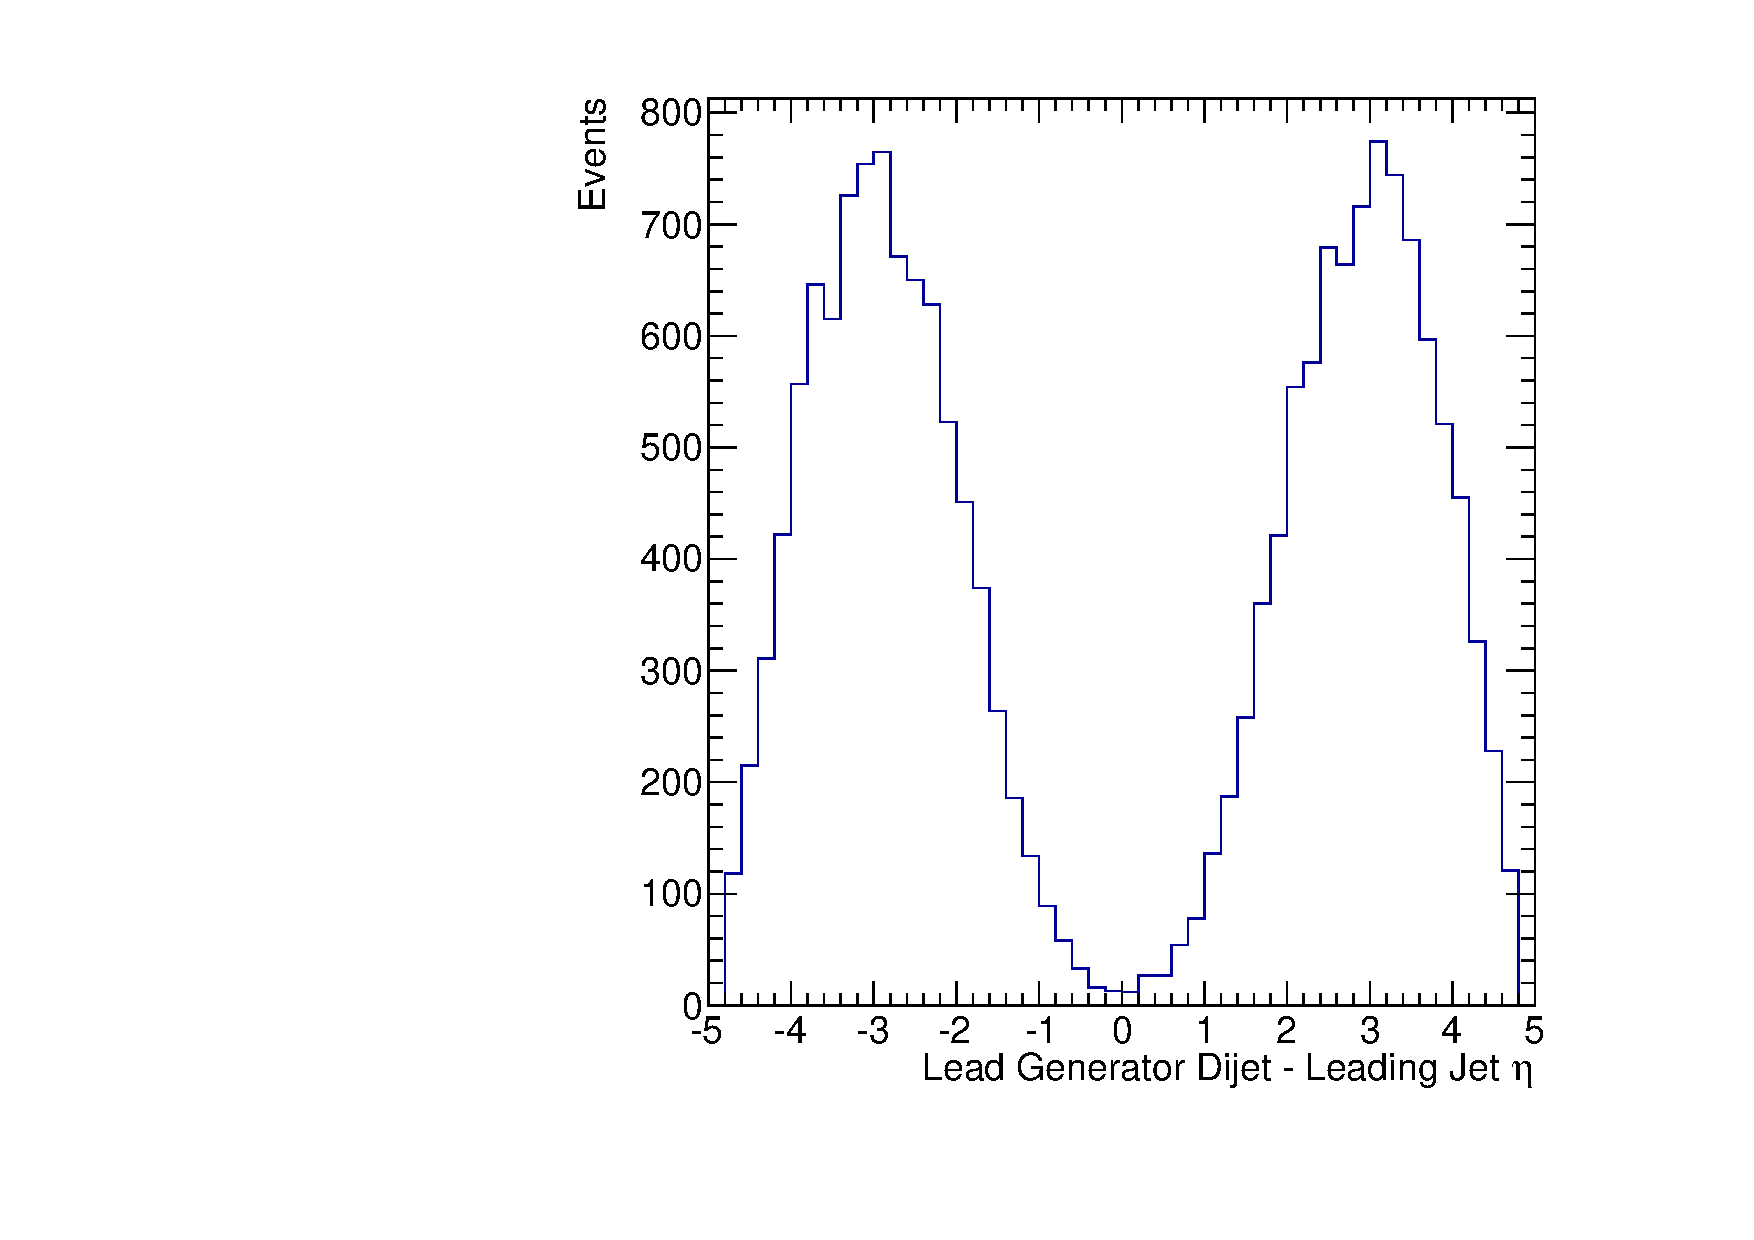
\includegraphics[width=0.40\linewidth]{Chapter08/QCDVBFSamples/GeneratorFilter/Pt40_Eta4p8_DEta3p0_Mjj1000/Images/LeadDijet_Jet0_Eta.pdf}}\qquad
\subfloat[][]{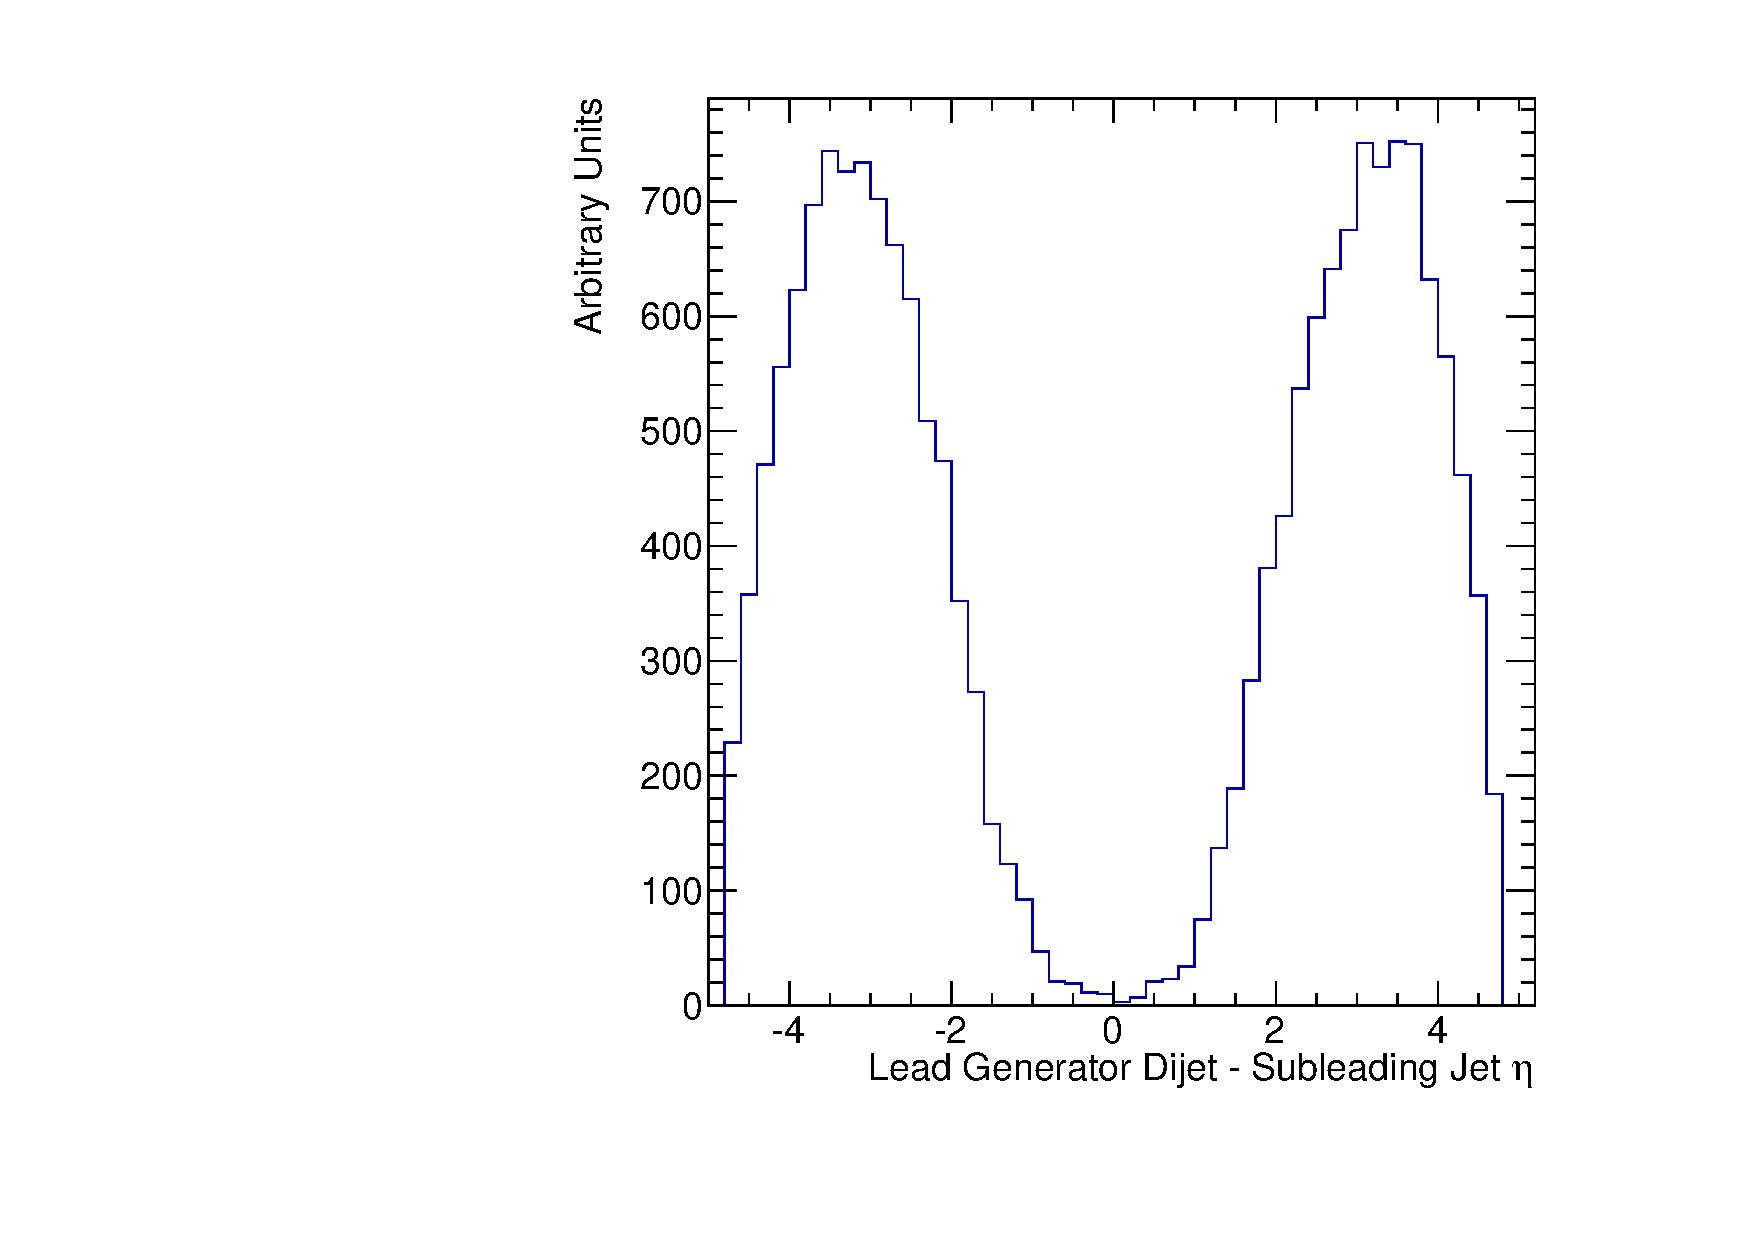
\includegraphics[width=0.40\linewidth]{Chapter08/QCDVBFSamples/GeneratorFilter/Pt40_Eta4p8_DEta3p0_Mjj1000/Images/LeadDijet_Jet1_Eta.pdf}}\\
\caption{Relevant distributions for the two jets comprising the the leading dijet passing a generator filter requiring at least one dijet with $\Delta\eta>3.0$ and $M_{jj}>1000\,\GeV$ where the jets have $\pt>40\,\GeV$ and $|\eta|<4.8$}
\label{FIGURE:RunIIPreparation_PassGeneratorFilterDistributions1}
\end{figure}

All the distributions show the expected features of the generator level filter cuts. As expected the peak of the $\Delta\phi$ distribution is at \pi when the 2 jets are back to back, but a tail of events is visible down to zero.

\begin{figure}[!htp]%
\centering
\subfloat[][]{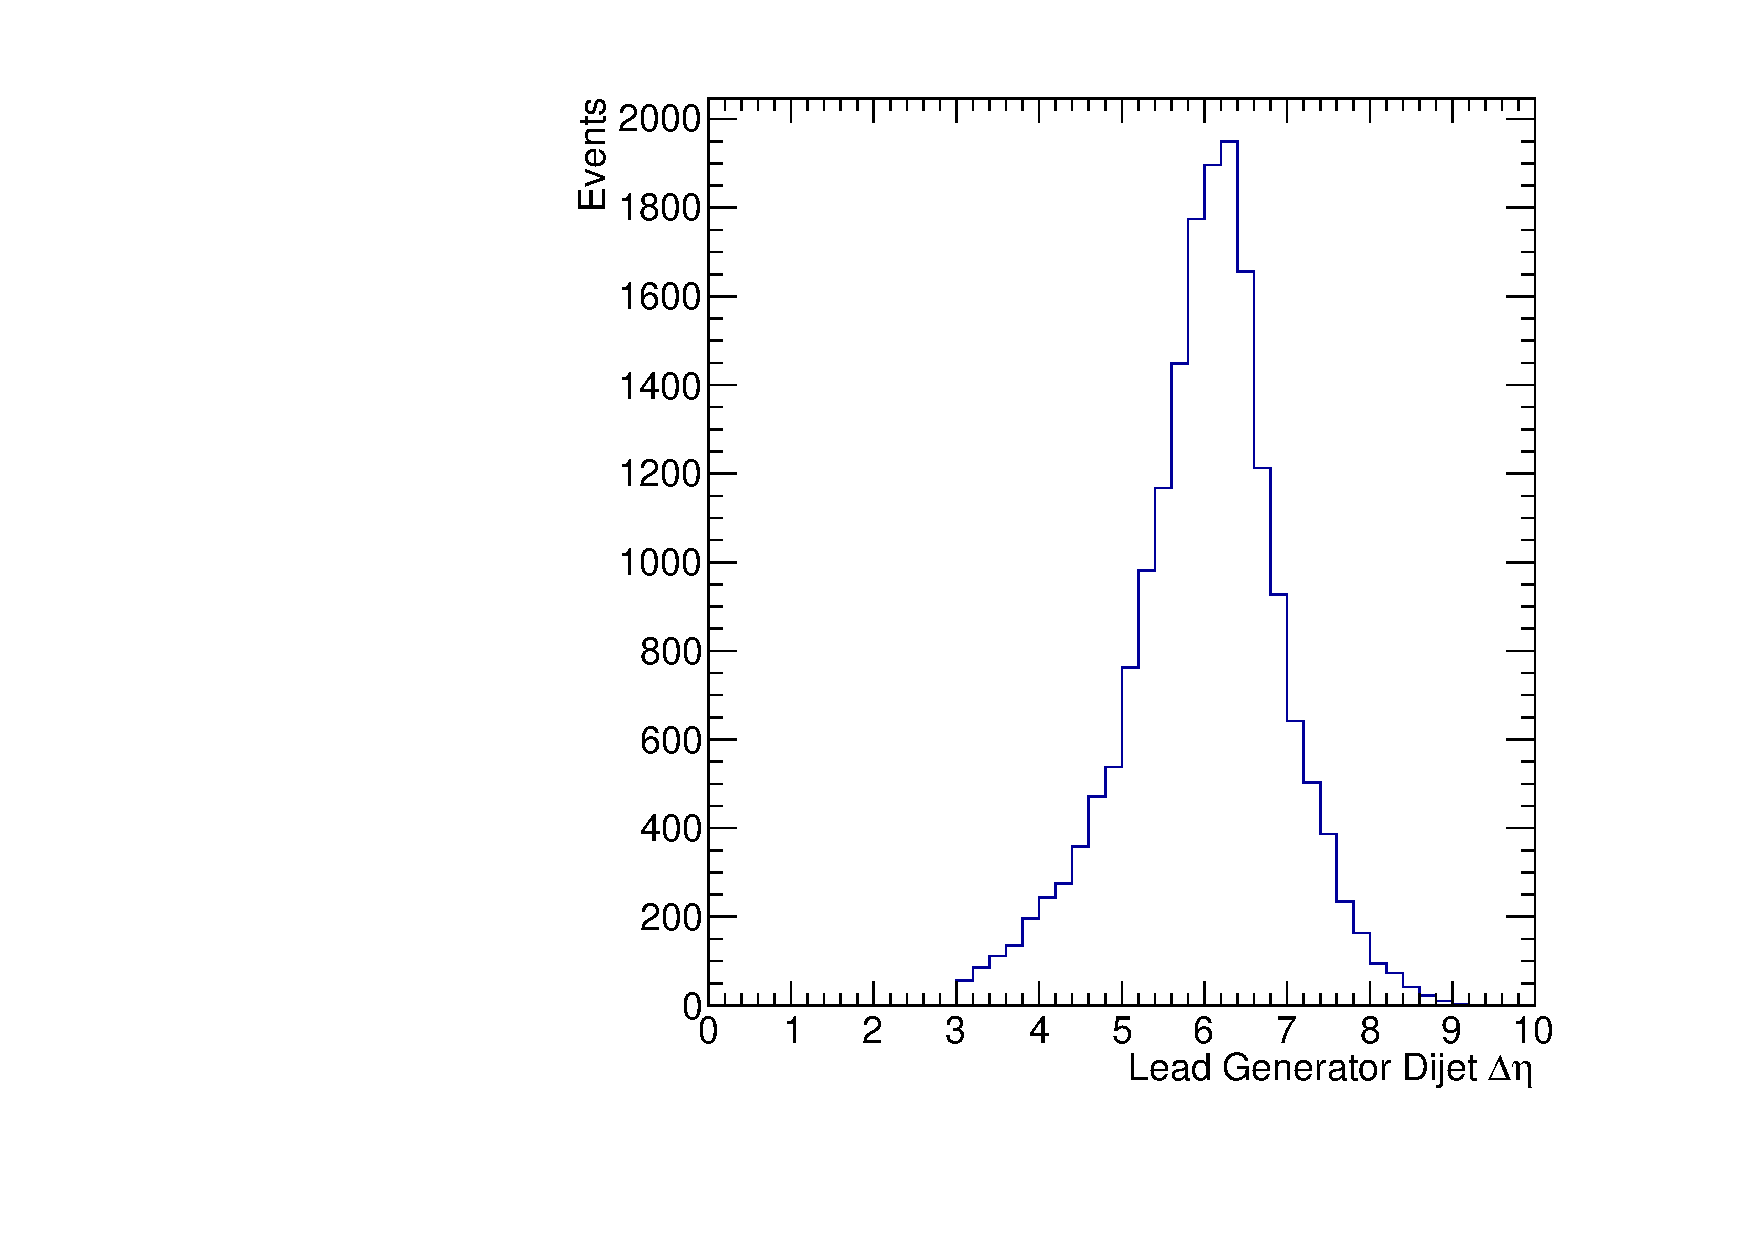
\includegraphics[width=0.40\linewidth]{Chapter08/QCDVBFSamples/GeneratorFilter/Pt40_Eta4p8_DEta3p0_Mjj1000/Images/LeadDijet_DEta.pdf}}\qquad
\subfloat[][]{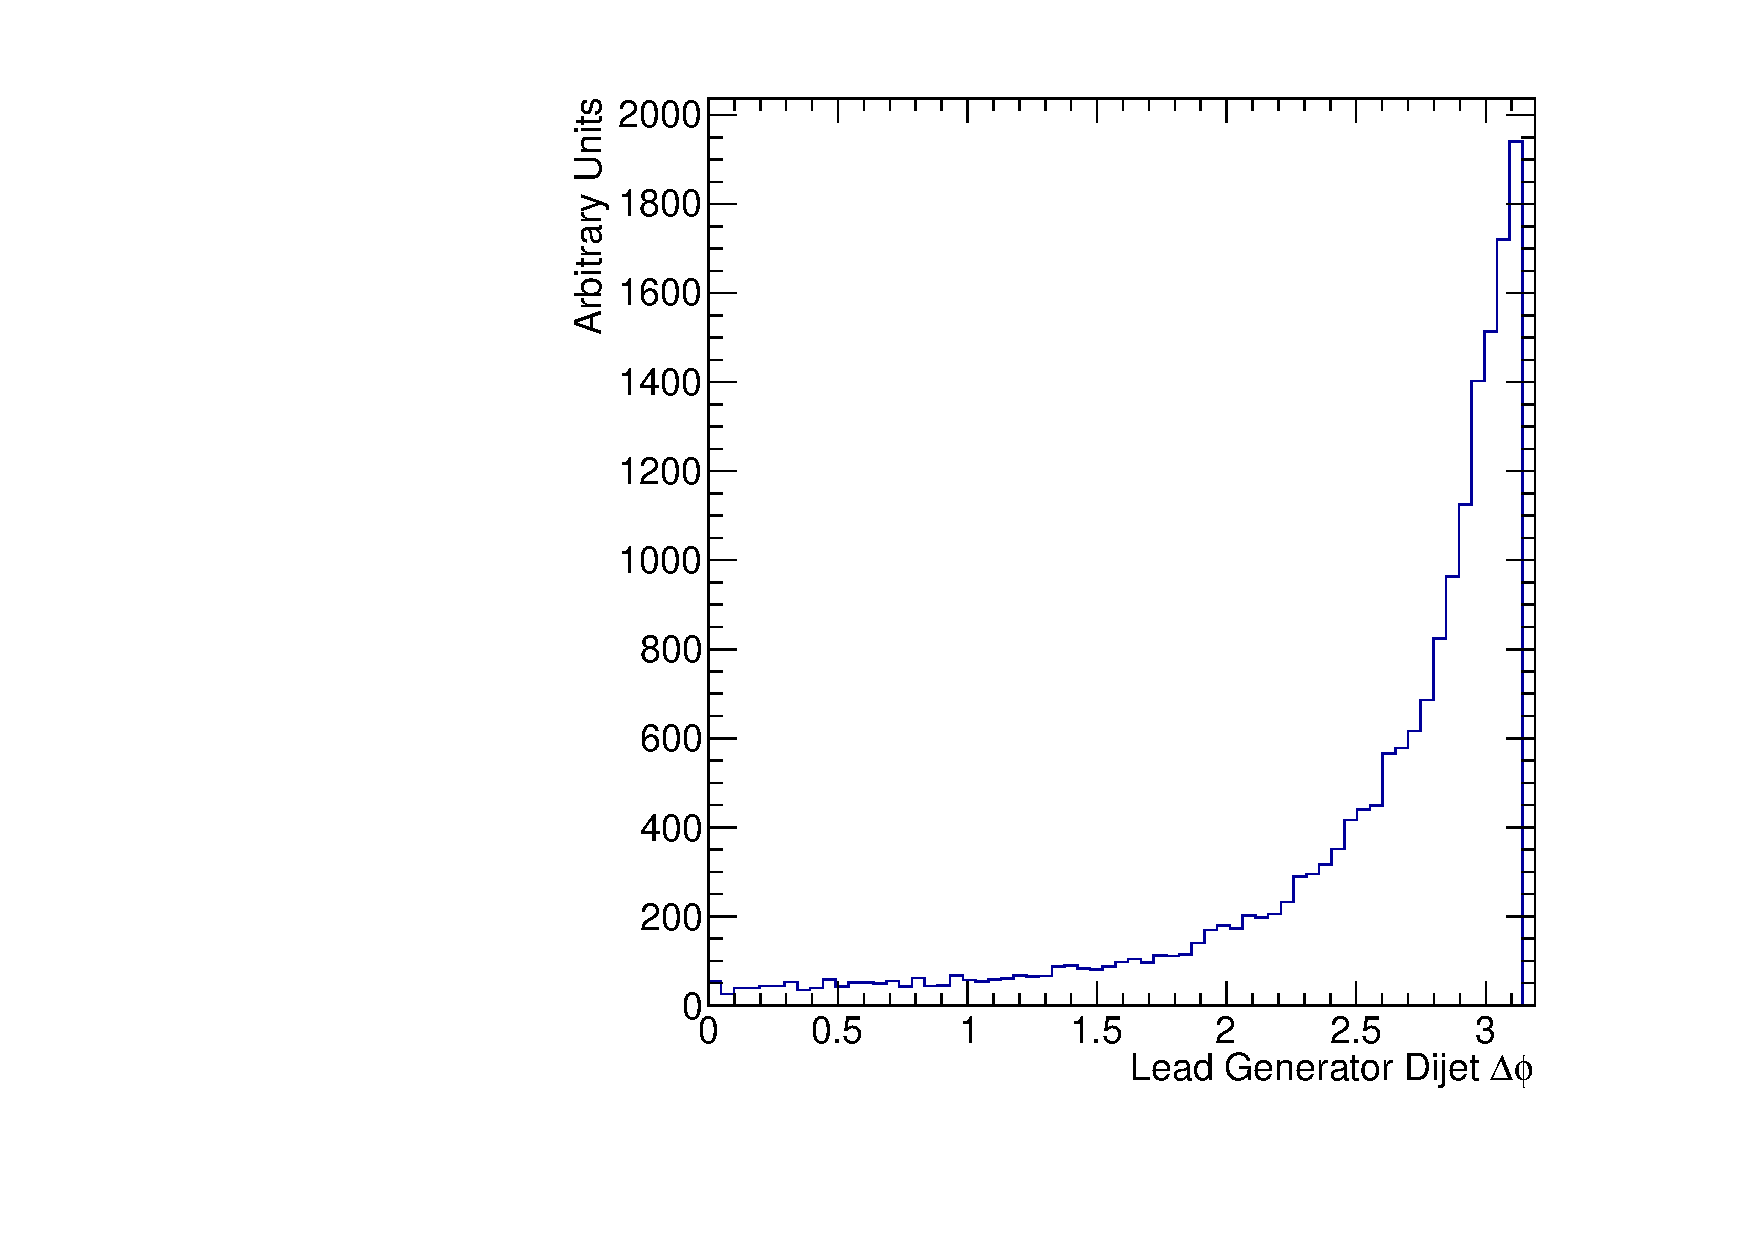
\includegraphics[width=0.40\linewidth]{Chapter08/QCDVBFSamples/GeneratorFilter/Pt40_Eta4p8_DEta3p0_Mjj1000/Images/LeadDijet_DPhi.pdf}}\\
\subfloat[][]{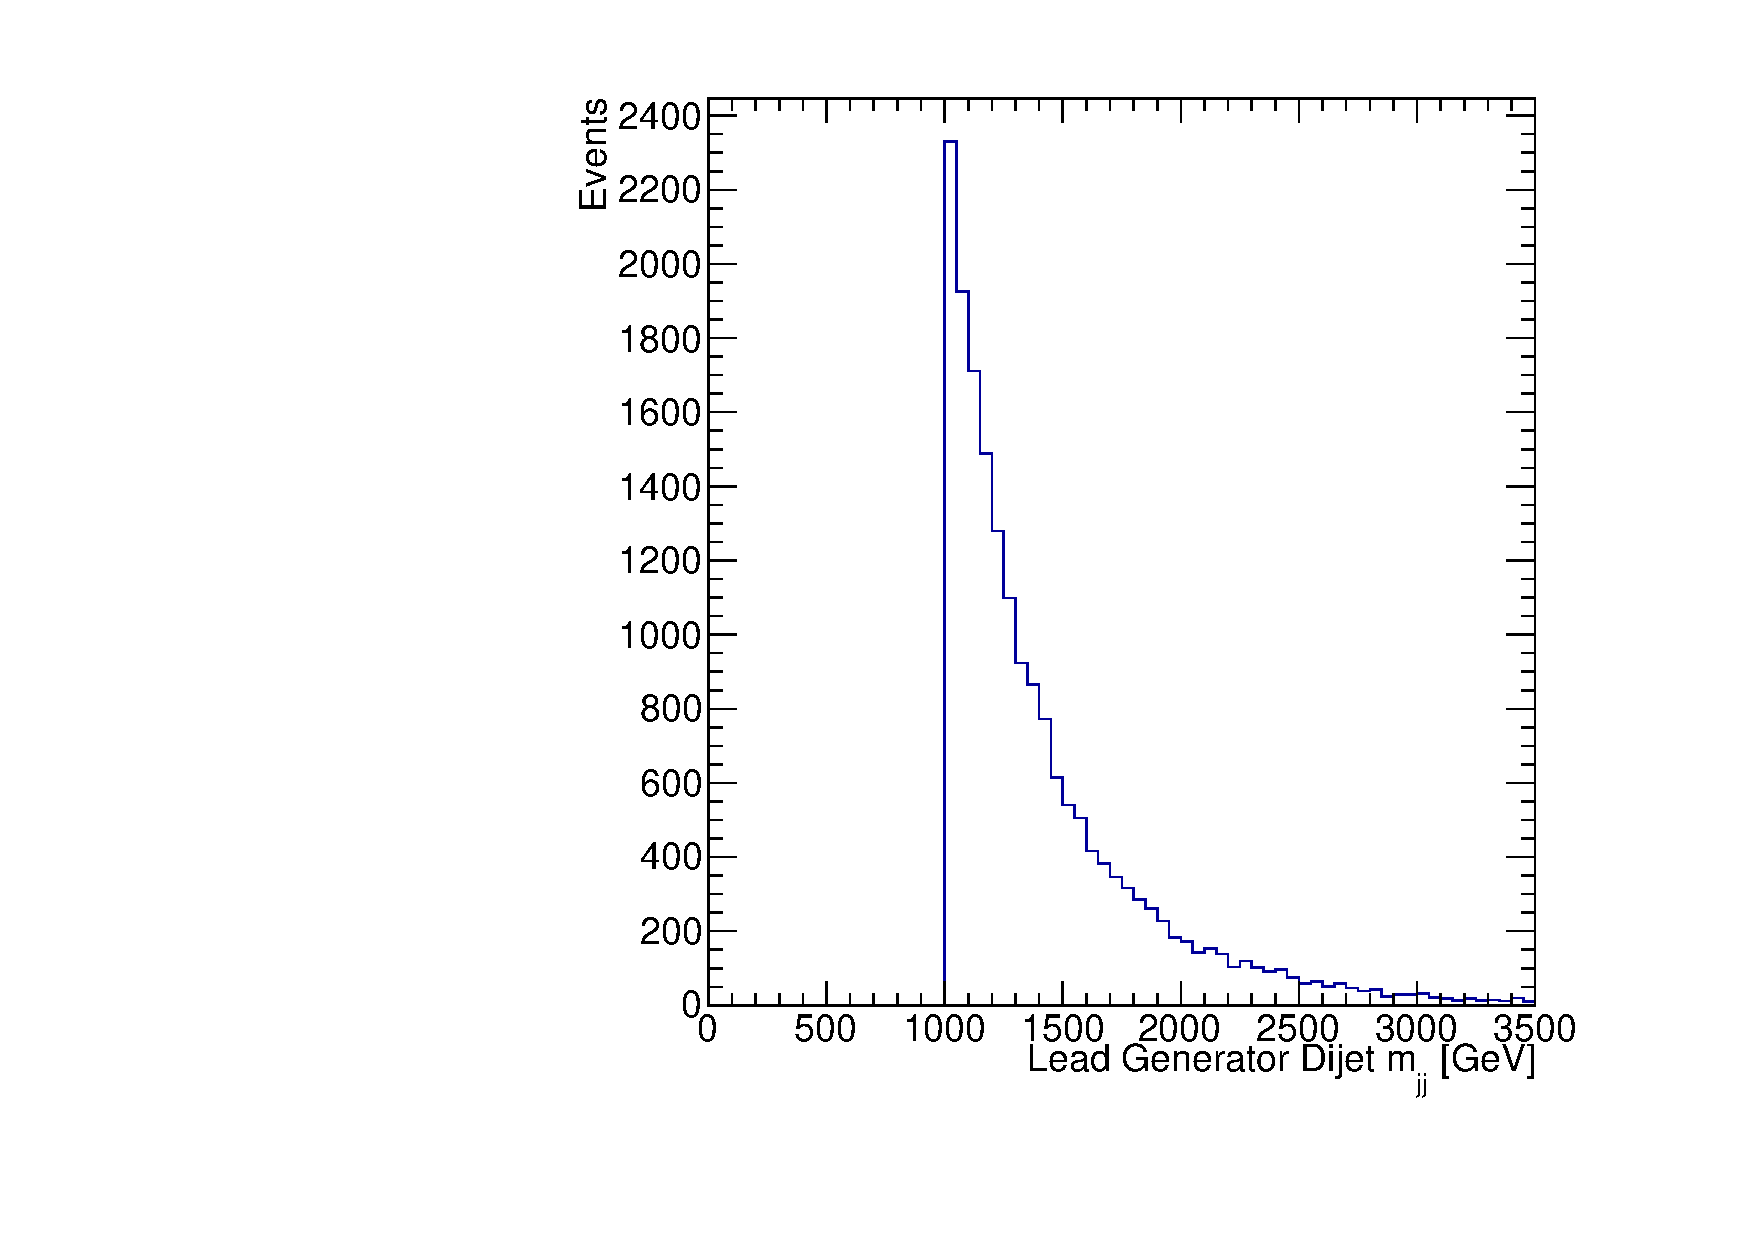
\includegraphics[width=0.40\linewidth]{Chapter08/QCDVBFSamples/GeneratorFilter/Pt40_Eta4p8_DEta3p0_Mjj1000/Images/LeadDijet_Mjj.pdf}}\\
\caption{Relevant distributions for the leading dijet passing a generator filter requiring at least one dijet with $\Delta\eta>3.0$ and $M_{jj}>1000\,\GeV$ where the jets have $\pt>40\,\GeV$ and $|\eta|<4.8$}
\label{FIGURE:RunIIPreparation_PassGeneratorFilterDistributions2}
\end{figure}

Sub-sample A will be produced by running over all the events produced up to the hadronization step. Its estimated filter efficiency is $(2.938 \pm 0.005) \times 10^{-1}$ which would lead to a sample size of approximately 29 million events and corresponding to an equivalent luminosity of over $1.1\,\femto\barn^{-1}$.

Sub-sample B will result from running over only 10\% of the events available at the hadronization step. This filter has an efficiency $(1.125 \pm 0.009) \times 10^{-1}$  and would lead to sample of about 14 million events, corresponding to an equivalent luminosity of over $110\,\pico\barn$. If additional computing resources would become available this sample could be expanded up to 100\% of the base sample to a total of 141 million events and equivalent luminosity over $1.1\,\femto\barn^{-1}$.

It is necessary to determine the overlap between these two sub-samples. From table \ref{TABLE:RunIIPreparation_PassFilterNJetsDphi}, we can see that a significant number of events of each sub-sample have additional jets, passing all required jet conditions. 

\begin{table}[!htp]
\centering
\begin{tabular}{|c||c|c|c|}
\hline
           & \multicolumn{3}{c|}{$\Delta\phi$ cut} \\
\hline
$N_{Jets}$ & no cut        & $<2.15$        & $\gtrsim 2.15$ \\
\hline\hline
 2         & 63.83 \pm 0.59 & 15.80 \pm 0.63 & 73.38 \pm 0.70 \\
 3         & 23.53 \pm 0.36 & 50.21 \pm 1.13 & 17.59 \pm 0.34 \\
 4         &  9.43 \pm 0.23 & 24.34 \pm 0.78 &  6.70 \pm 0.21 \\
 5         &  2.42 \pm 0.11 &  7.14 \pm 0.42 &  1.70 \pm 0.11 \\
+6         &  0.79 \pm 0.07 &  2.50 \pm 0.25 &  0.63 \pm 0.06 \\
\hline
\end{tabular}
\caption[Table showing the percentage of events for a given multiplicity of generator anti-$k_T$ jets with $R=0.4$ passing cuts $p_T>40\,\GeV$ and $|\eta|<4.8$. Only events with at least one such dijet with $\Delta\eta<3.0$ and $m_{jj}<1000\,\GeV$ are considered and results are presented according to a possible additional dijet $\Delta\phi$ cut.]
{Table showing the percentage of events for a given multiplicity of generator anti-$k_T$ jets with $R=0.4$ passing cuts $p_T>40\,\GeV$ and $|\eta|<4.8$. Only events with at least one such dijet with $\Delta\eta<3.0$ and $m_{jj}<1000\,\GeV$ are considered and results are presented according to a possible additional dijet $\Delta\phi$ cut.}
\label{TABLE:RunIIPreparation_PassFilterNJetsDphi}
\end{table}

% Information extracted to do this table:
%#######################################################
% Printing cuts: Pt40_Eta4p8_DEta3p0_Mjj1000
%#######################################################
% => Number Jets Passing pT and Eta cuts multiplicity (at least one combination passes all cuts):
% N_Jets= 0 entries=         0 fraction=0.000000 +/- 0.000000
% N_Jets= 1 entries=         0 fraction=0.000000 +/- 0.000000
% N_Jets= 2 entries=     11757 fraction=0.638274 +/- 0.005887
% N_Jets= 3 entries=      4335 fraction=0.235342 +/- 0.003574
% N_Jets= 4 entries=      1737 fraction=0.094300 +/- 0.002263
% N_Jets= 5 entries=       446 fraction=0.024213 +/- 0.001147
% N_Jets= 6 entries=       117 fraction=0.006352 +/- 0.000587
% N_Jets= 7 entries=        22 fraction=0.001194 +/- 0.000255
% N_Jets= 8 entries=         4 fraction=0.000217 +/- 0.000109
% N_Jets= 9 entries=         2 fraction=0.000109 +/- 0.000077
% N_Jets=10 entries=         0 fraction=0.000000 +/- 0.000000
%####################################################### 
% N_Jets=+6 entries=       145 fraction=0.007872 +/- 0.000654
%#######################################################
%
%
%######################################################
%Printing cuts: Pt40_Eta4p8_DEta3p0_Dphi2p15_Mjj1000
%######################################################
% => Number Jets Passing pT and Eta cuts multiplicity (at least one combination passes all cuts):
% N_Jets= 0 entries=         0 fraction=0.000000 +/- 0.000000
% N_Jets= 1 entries=         0 fraction=0.000000 +/- 0.000000
% N_Jets= 2 entries=       626 fraction=0.158041 +/- 0.006317
% N_Jets= 3 entries=      1989 fraction=0.502146 +/- 0.011259
% N_Jets= 4 entries=       964 fraction=0.243373 +/- 0.007839
% N_Jets= 5 entries=       283 fraction=0.071447 +/- 0.004247
% N_Jets= 6 entries=        81 fraction=0.020449 +/- 0.002272
% N_Jets= 7 entries=        15 fraction=0.003787 +/- 0.000978
% N_Jets= 8 entries=         2 fraction=0.000505 +/- 0.000357
% N_Jets= 9 entries=         1 fraction=0.000252 +/- 0.000252
% N_Jets=10 entries=         0 fraction=0.000000 +/- 0.000000
%####################################################### 
% N_Jets=+6 entries=        99 fraction=0.024994 +/- 0.002512
%####################################################### 
%
%
%#######################################################
%Printing cuts: Pt40_Eta4p8_DEta3p0_MinDphi2p15_Mjj1000
%####################################################### 
% => Number Jets Passing pT and Eta cuts multiplicity (at least one combination passes all cuts):
% N_Jets= 0 entries=         0 fraction=0.000000 +/- 0.000000
% N_Jets= 1 entries=         0 fraction=0.000000 +/- 0.000000
% N_Jets= 2 entries=     11131 fraction=0.733799 +/- 0.006955
% N_Jets= 3 entries=      2668 fraction=0.175885 +/- 0.003405
% N_Jets= 4 entries=      1017 fraction=0.067045 +/- 0.002102
% N_Jets= 5 entries=       258 fraction=0.017008 +/- 0.001059
% N_Jets= 6 entries=        75 fraction=0.004944 +/- 0.000571
% N_Jets= 7 entries=        15 fraction=0.000989 +/- 0.000255
% N_Jets= 8 entries=         3 fraction=0.000198 +/- 0.000114
% N_Jets= 9 entries=         2 fraction=0.000132 +/- 0.000093
% N_Jets=10 entries=         0 fraction=0.000000 +/- 0.000000
%#######################################################
% N_Jets=+6 entries=        95 fraction=0.006263 +/- 0.000643
%#######################################################


These additional jets lead to additional combinations that may pass the criteria of the opposite sub-sample. As it can be seen in table \ref{TABLE:RunIIPreparation_PassFilterNDijetsDphi} in as much as 5\% of the events in the $\Delta\phi \leq 2.15$ sub-sample there is a second combination of two jets that would pass the criteria to be in that sub-sample.

\begin{table}[!htp]
\centering
\begin{tabular}{|c|c|c|c|}
\hline
           & \multicolumn{3}{c|}{$\Delta\phi$ cut} \\
\hline
$N_{Jets}$ & no cut        & $<2.15$        & $\gtrsim 2.15$ \\
\hline\hline
 1         & 93.53 \pm 0.71 & 94.29 \pm 1.54 & 97.51 \pm 0.80 \\
 2         &  5.84 \pm 0.18 &  5.35 \pm 0.37 &  2.39 \pm 0.13 \\
 3         &  0.44 \pm 0.05 &  0.30 \pm 0.09 &  0.07 \pm 0.02 \\
+4         &  0.19 \pm 0.03 &  0.05 \pm 0.04 &  0.03 \pm 0.01 \\
\hline
\end{tabular}
\caption{Table showing the percentage of generator AK4 dijets passing cuts $p_T^{jet}>40\,\GeV$, $|\eta|^{jet}<4.8$, $\Delta\eta<3.0$ and $m_{jj}<1000\,\GeV$ and according to an additional dijet $\Delta\phi$ cut.}
\end{table}

% #######################################################
% Printing cuts: Pt40_Eta4p8_DEta3p0_Mjj1000
% #######################################################
% => Dijets passing all cuts multiplicity:
% N_Dijets= 0 entries=         0 fraction=0.000000 +/- 0.000000
% N_Dijets= 1 entries=     17228 fraction=0.935288 +/- 0.007126
% N_Dijets= 2 entries=      1076 fraction=0.058415 +/- 0.001781
% N_Dijets= 3 entries=        81 fraction=0.004397 +/- 0.000489
% N_Dijets= 4 entries=        31 fraction=0.001683 +/- 0.000302
% N_Dijets= 5 entries=         2 fraction=0.000109 +/- 0.000077
% N_Dijets= 6 entries=         2 fraction=0.000109 +/- 0.000077
% N_Dijets= 7 entries=         0 fraction=0.000000 +/- 0.000000
% N_Dijets= 8 entries=         0 fraction=0.000000 +/- 0.000000
% N_Dijets= 9 entries=         0 fraction=0.000000 +/- 0.000000
% N_Dijets=10 entries=         0 fraction=0.000000 +/- 0.000000
% ####################################################### 
% N_Dijets=+4 entries=        35 fraction=0.001900 +/- 0.000321
% #######################################################
%
% 
% #######################################################
% Printing cuts: Pt40_Eta4p8_DEta3p0_Dphi2p15_Mjj1000
% #######################################################
% => Dijets passing all cuts multiplicity:
% N_Dijets= 0 entries=         0 fraction=0.000000 +/- 0.000000
% N_Dijets= 1 entries=      3735 fraction=0.942944 +/- 0.015429
% N_Dijets= 2 entries=       212 fraction=0.053522 +/- 0.003676
% N_Dijets= 3 entries=        12 fraction=0.003030 +/- 0.000875
% N_Dijets= 4 entries=         2 fraction=0.000505 +/- 0.000357
% N_Dijets= 5 entries=         0 fraction=0.000000 +/- 0.000000
% N_Dijets= 6 entries=         0 fraction=0.000000 +/- 0.000000
% N_Dijets= 7 entries=         0 fraction=0.000000 +/- 0.000000
% N_Dijets= 8 entries=         0 fraction=0.000000 +/- 0.000000
% N_Dijets= 9 entries=         0 fraction=0.000000 +/- 0.000000
% N_Dijets=10 entries=         0 fraction=0.000000 +/- 0.000000
% ####################################################### 
%
% #######################################################
% 
% 
% #######################################################
% Printing cuts: Pt40_Eta4p8_DEta3p0_MinDphi2p15_Mjj1000
% #######################################################
% => Dijets passing all cuts multiplicity:
% N_Dijets= 0 entries=         0 fraction=0.000000 +/- 0.000000
% N_Dijets= 1 entries=     14791 fraction=0.975081 +/- 0.008018
% N_Dijets= 2 entries=       363 fraction=0.023930 +/- 0.001256
% N_Dijets= 3 entries=        11 fraction=0.000725 +/- 0.000219
% N_Dijets= 4 entries=         4 fraction=0.000264 +/- 0.000132
% N_Dijets= 5 entries=         0 fraction=0.000000 +/- 0.000000
% N_Dijets= 6 entries=         0 fraction=0.000000 +/- 0.000000
% N_Dijets= 7 entries=         0 fraction=0.000000 +/- 0.000000
% N_Dijets= 8 entries=         0 fraction=0.000000 +/- 0.000000
% N_Dijets= 9 entries=         0 fraction=0.000000 +/- 0.000000
% N_Dijets=10 entries=         0 fraction=0.000000 +/- 0.000000
% ####################################################### 
%
% #######################################################


The overlap between the two sub-samples has been determined to be $3.95\% \pm 0.14\%$ of the events passing the initial selection. Since this number is relevant, and to avoid event double counting, events with combinations that would pass both sub-sample definitions should be selected into the smallest equivalent luminosity sub-sample.

%%%%%%%%%%%%%%%%%%%%%%%%%%%%%%%%%%%%%%%%%%%%%%%%%%%%%%%%%%%%%%%%%%%%%%%%%%%%%%%%%%%%%%%
%%% SUBSECTION
%%%%%%%%%%%%%%%%%%%%%%%%%%%%%%%%%%%%%%%%%%%%%%%%%%%%%%%%%%%%%%%%%%%%%%%%%%%%%%%%%%%%%%%
\subsection{Migration study}
\label{SUBSECTION:RunIIPreparation_MigrationStudy}

%Status: DONE (reviewed J.Pela x1)

One concern when making cuts at steps below event reconstruction is the possibility of removing events that may pass analysis level event selections. This migration of events needs to be taken into account while defining the requirements at parton and generator levels. The signal region selection used during the 2012-13 parked data analysis selected events with a dijet passing $\Delta\eta>3.6$, $M_{jj}>1200\,\GeV$ where the lead jet $\pt > 50\,\GeV$ and sub-lead jet $\pt > 45\,\GeV$ and both have $|\eta|<4.7$ (condition to guarantee the used AK5 jets are fully contained in the detector). It is unlikely that the Run II offline selection would be able to cut below jet $\pt > 50\,\GeV$.

In order to study migration, a second \gls{MC} sample with lower parton cuts was generated. \textsc{MADGRAPH} was used again to generate events with the same parameters with the only difference being the dijet cuts. Events are selected with at least a pair of outgoing partons with invariant mass of $600\,\GeV$, where both partons are inside the detector volume with $|\eta|<5.0$ and $p_{T}>10\,\GeV$. Hadronization was then performed with the same procedure described in the previous section.

In order to compare generator jets to the partons that created them, matching is needed. For each parton, all generator jet, are selected which are located at $\Delta R < 0.4$ and from those we select the generator jet closest in \pt to the selected parton. This procedure attempts to account for the situation where more than one jet is within the matching distance, but the best match in \pt is not the closest one in $\Delta R$. Using this procedure, a match for the di-parton passing the imposed cuts can be found for 73.24\% of the events and the matched generator jet is not the closest one in $\Delta R$ for 3.45\% of the partons. A table of the matching efficiency discriminated by physics process can be found in table \ref{TABLE:RunIIPreparation_PartonGenJetMatchingEfficiency}. 

\begin{table}[!htp]
\centering

\begin{tabular}{|c||c|c|c||c|}
\hline
            &          \multicolumn{4}{c|}{Process} \\
\hline
$n_{match}$ &      jj &    jjj  &    jjjj &   Total \\
\hline\hline 
          0 & 22.04\% \pm 0.22\%  &  2.18\% \pm  0.09\% &  0.14\% \pm  0.03\% & 11.62\% \pm 0.11\% \\
          1 & 38.60\% \pm 0.30\%  & 17.82\% \pm  0.25\% &  3.02\% \pm  0.13\% & 25.27\% \pm 0.17\% \\
          2 & 39.35\% \pm 0.30\%  & 42.35\% \pm  0.39\% & 16.91\% \pm  0.32\% & 35.99\% \pm 0.20\% \\
          3 &                     & 37.65\% \pm  0.37\% & 41.88\% \pm  0.50\% & 19.83\% \pm 0.15\% \\
          4 &                     &                     & 38.05\% \pm  0.47\% &  7.29\% \pm 0.09\% \\
\hline
\end{tabular}
\caption{Table showing the percentage of partons successfully matched to a generator AK4 jets. Numbers obtained for a total of 88282 events over all 3 possible hard scattering processes and for events with at least on di-parton with $m_{jj}>600\,GeV$ where each parton has $\pt < 10\,\GeV$ and $|\eta|<5.0$}
\label{TABLE:RunIIPreparation_PartonGenJetMatchingEfficiency}
\end{table}               

% => Parton to GenJet matching results:                                                                                                                                       
% all partons entries 88282                                                                                                                                                   
% Matched #0 partons:  10257 percentage: 11.62 +/-  0.11                                                                                                                      
% Matched #1 partons:  22308 percentage: 25.27 +/-  0.17                                                                                                                      
% Matched #2 partons:  31771 percentage: 35.99 +/-  0.20                                                                                                                      
% Matched #3 partons:  17506 percentage: 19.83 +/-  0.15                                                                                                                      
% Matched #4 partons:   6440 percentage:  7.29 +/-  0.09                                                                                                                      
% 
% jj partons entries 43689                                                                                                                                                    
% Matched #0 partons:   9631 percentage: 22.04 +/-  0.22                                                                                                                      
% Matched #1 partons:  16866 percentage: 38.60 +/-  0.30                                                                                                                      
% Matched #2 partons:  17192 percentage: 39.35 +/-  0.30                                                                                                                      
% 
% jjj partons entries 27667                                                                                                                                                   
% Matched #0 partons:    603 percentage:  2.18 +/-  0.09                                                                                                                      
% Matched #1 partons:   4930 percentage: 17.82 +/-  0.25                                                                                                                      
% Matched #2 partons:  11716 percentage: 42.35 +/-  0.39                                                                                                                      
% Matched #3 partons:  10418 percentage: 37.65 +/-  0.37                                                                                                                      
% 
% jjjj partons entries 16926                                                                                                                                                  
% Matched #0 partons:     23 percentage:  0.14 +/-  0.03                                                                                                                      
% Matched #1 partons:    512 percentage:  3.02 +/-  0.13                                                                                                                      
% Matched #2 partons:   2863 percentage: 16.91 +/-  0.32                                                                                                                      
% Matched #3 partons:   7088 percentage: 41.88 +/-  0.50                                                                                                                      
% Matched #4 partons:   6440 percentage: 38.05 +/-  0.47 




Partons are being simulated with fairly low \pt, two jets with $\pt > 10\,\GeV$ and up to two more with no restriction on energy. It is not a surprise that in significant number of events all partons cannot be matched to generator jets. This is due to the spread of energy over a larger area than the jet algorithm can cluster and due to the default AK4 minimum \pt necessary to form a jet of $3\,\GeV$. A set of plots of the relevant variables is shown in figure \ref{FIGURE:RunIIPreparation_VariablesPartonVsGenJet}. The selected di-partons are taken and each variable is plotted against the matched dijet.


\begin{figure}[!htp]%
\centering
\subfloat[][]{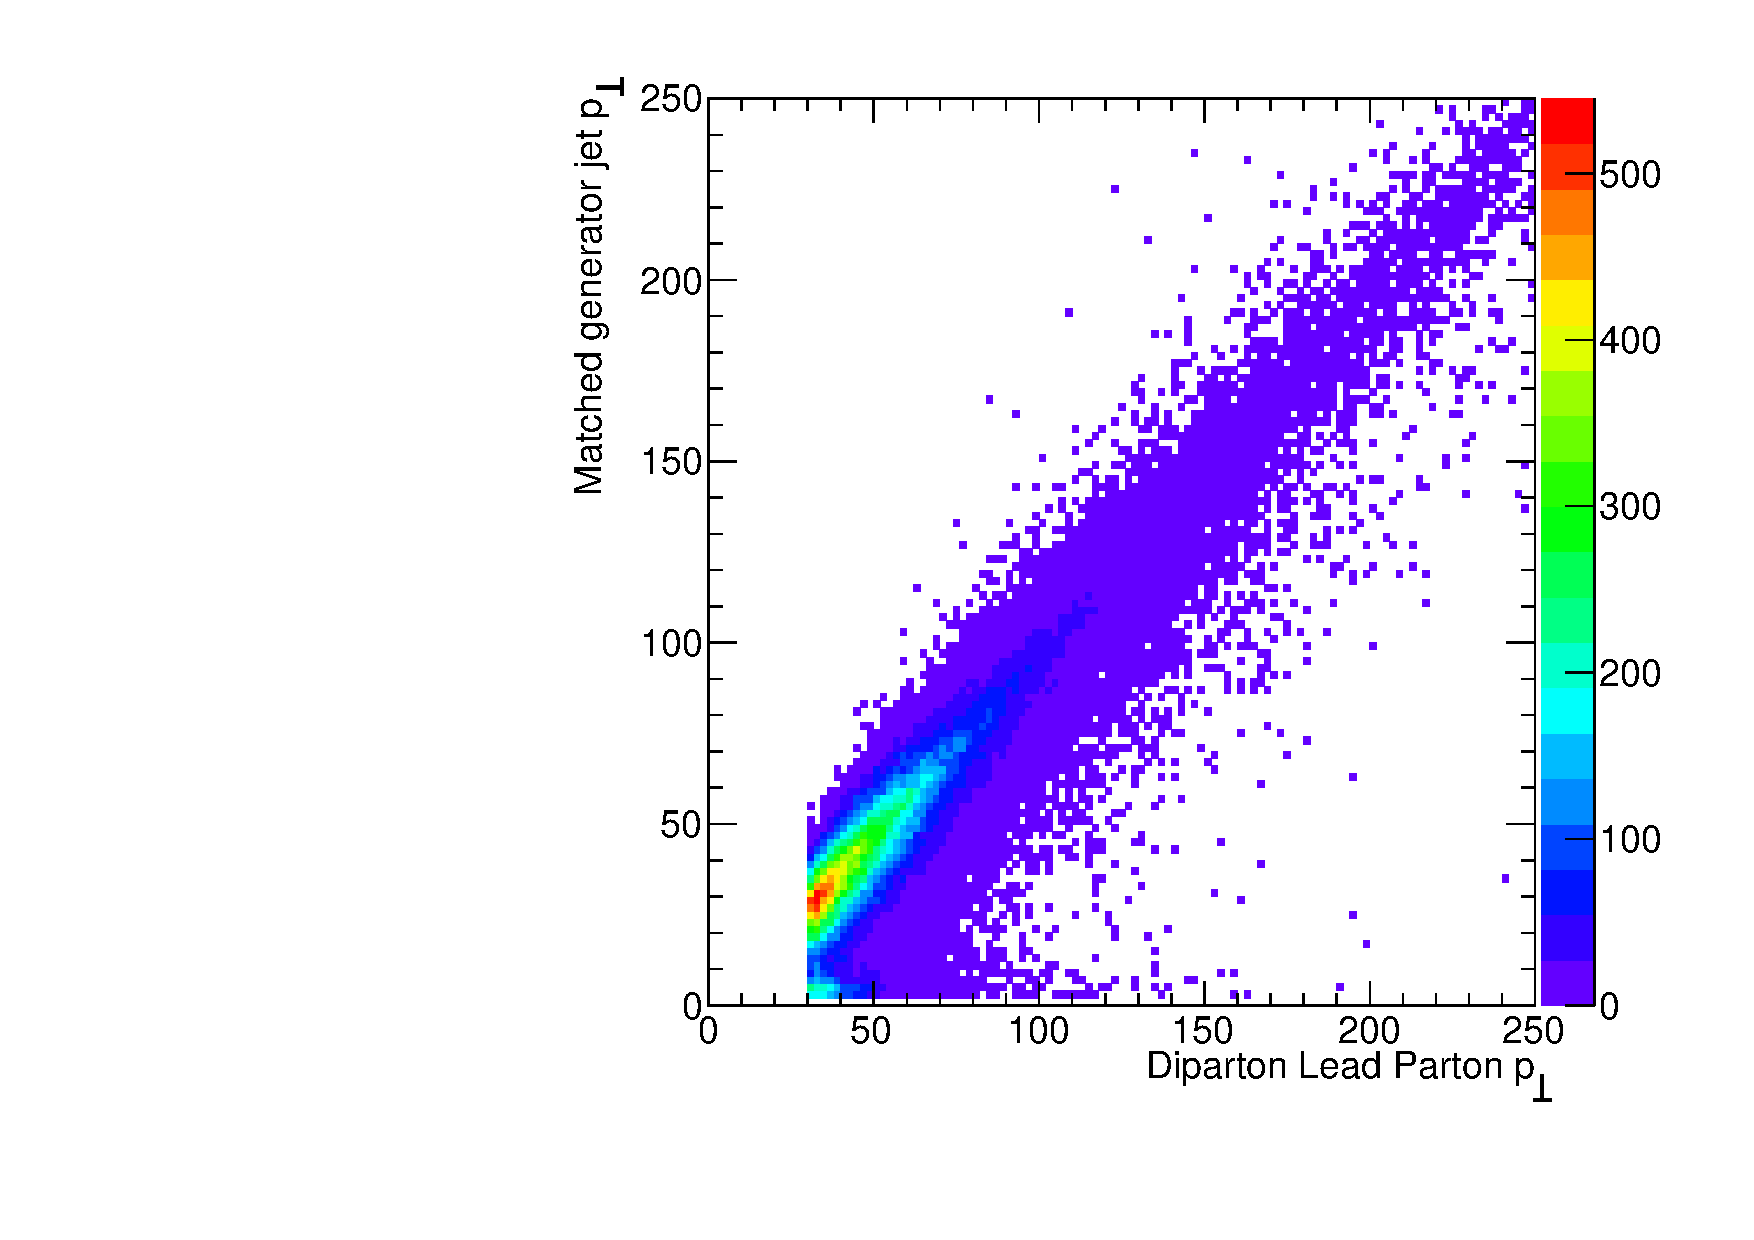
\includegraphics[width=0.40\linewidth]{Chapter08/QCDVBFSamples/Migrations/Images/SelDiParton_MatchedGenJet_Parton1_Pt.pdf}}\qquad
\subfloat[][]{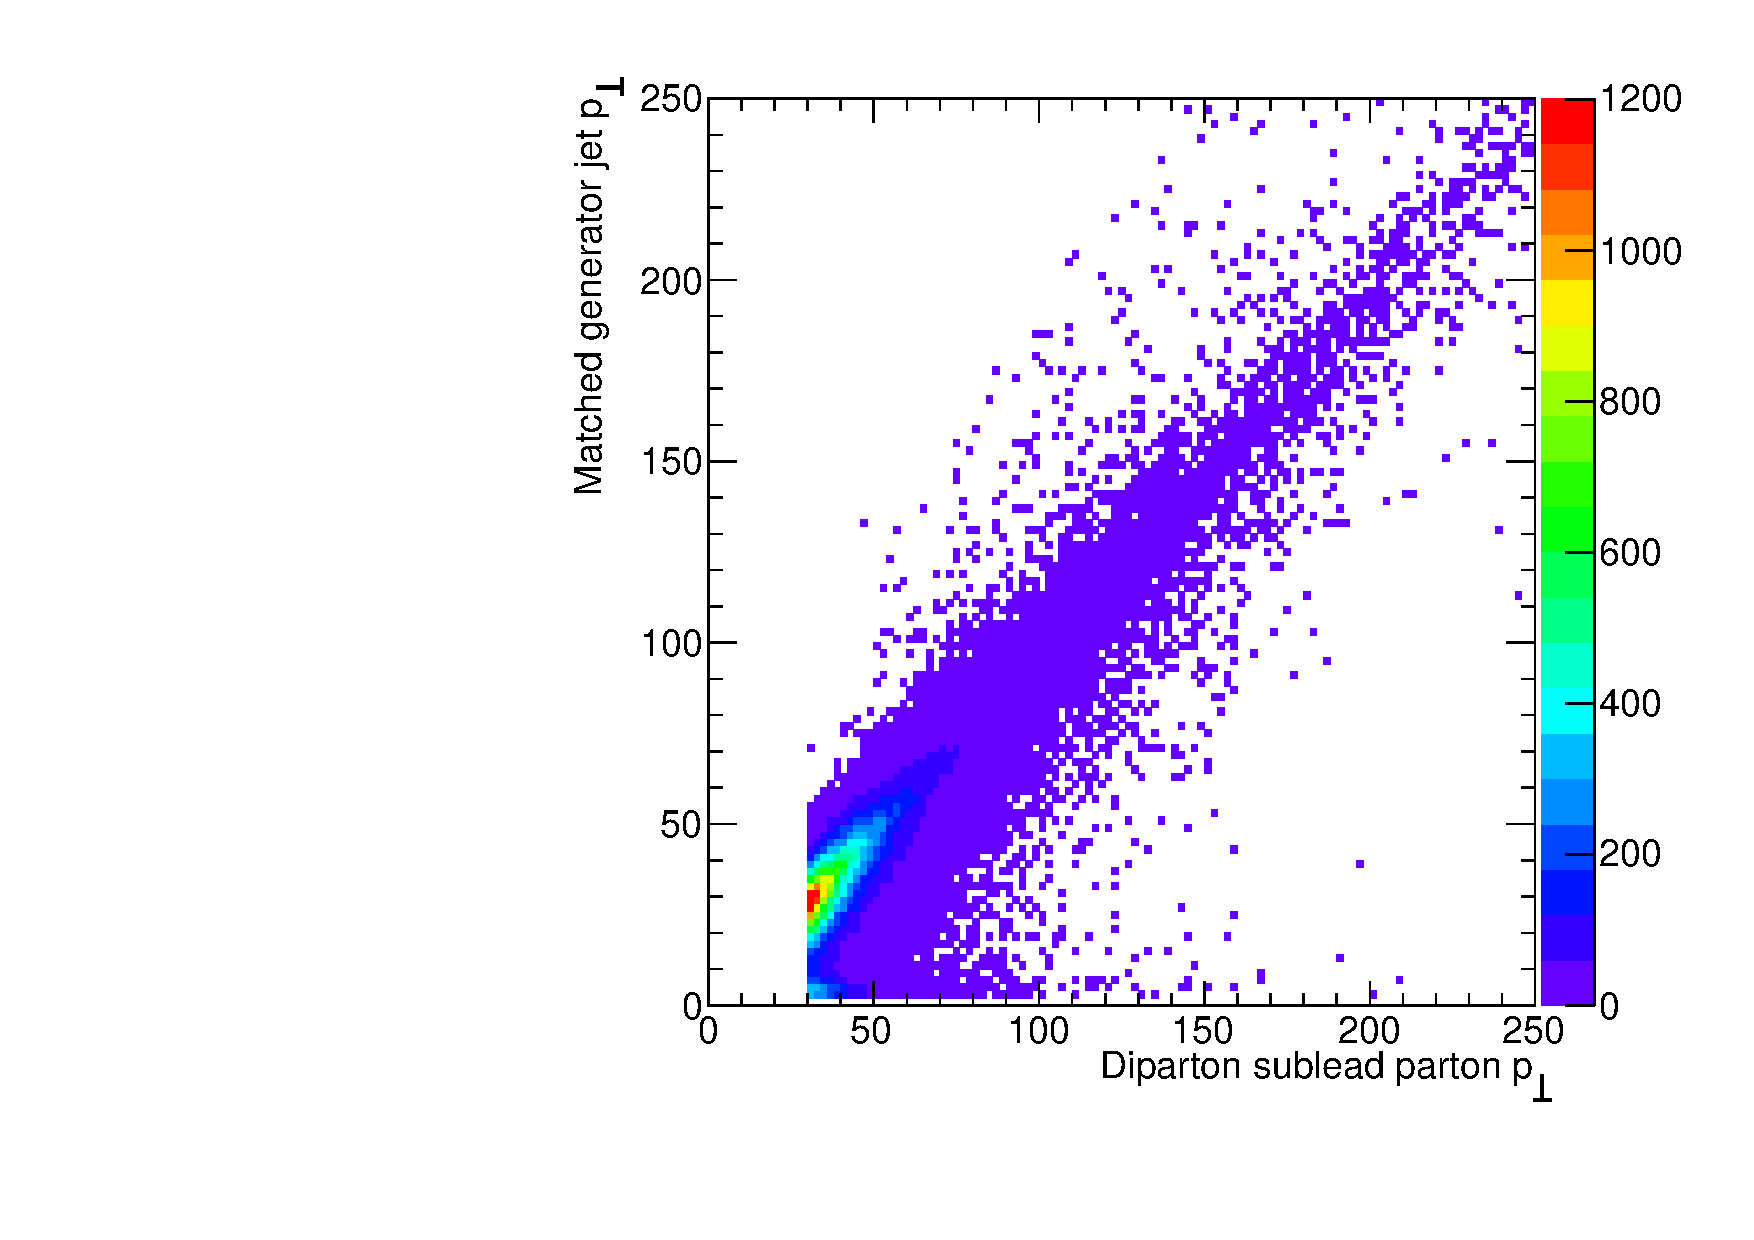
\includegraphics[width=0.40\linewidth]{Chapter08/QCDVBFSamples/Migrations/Images/SelDiParton_MatchedGenJet_Parton2_Pt.pdf}}\\
\subfloat[][]{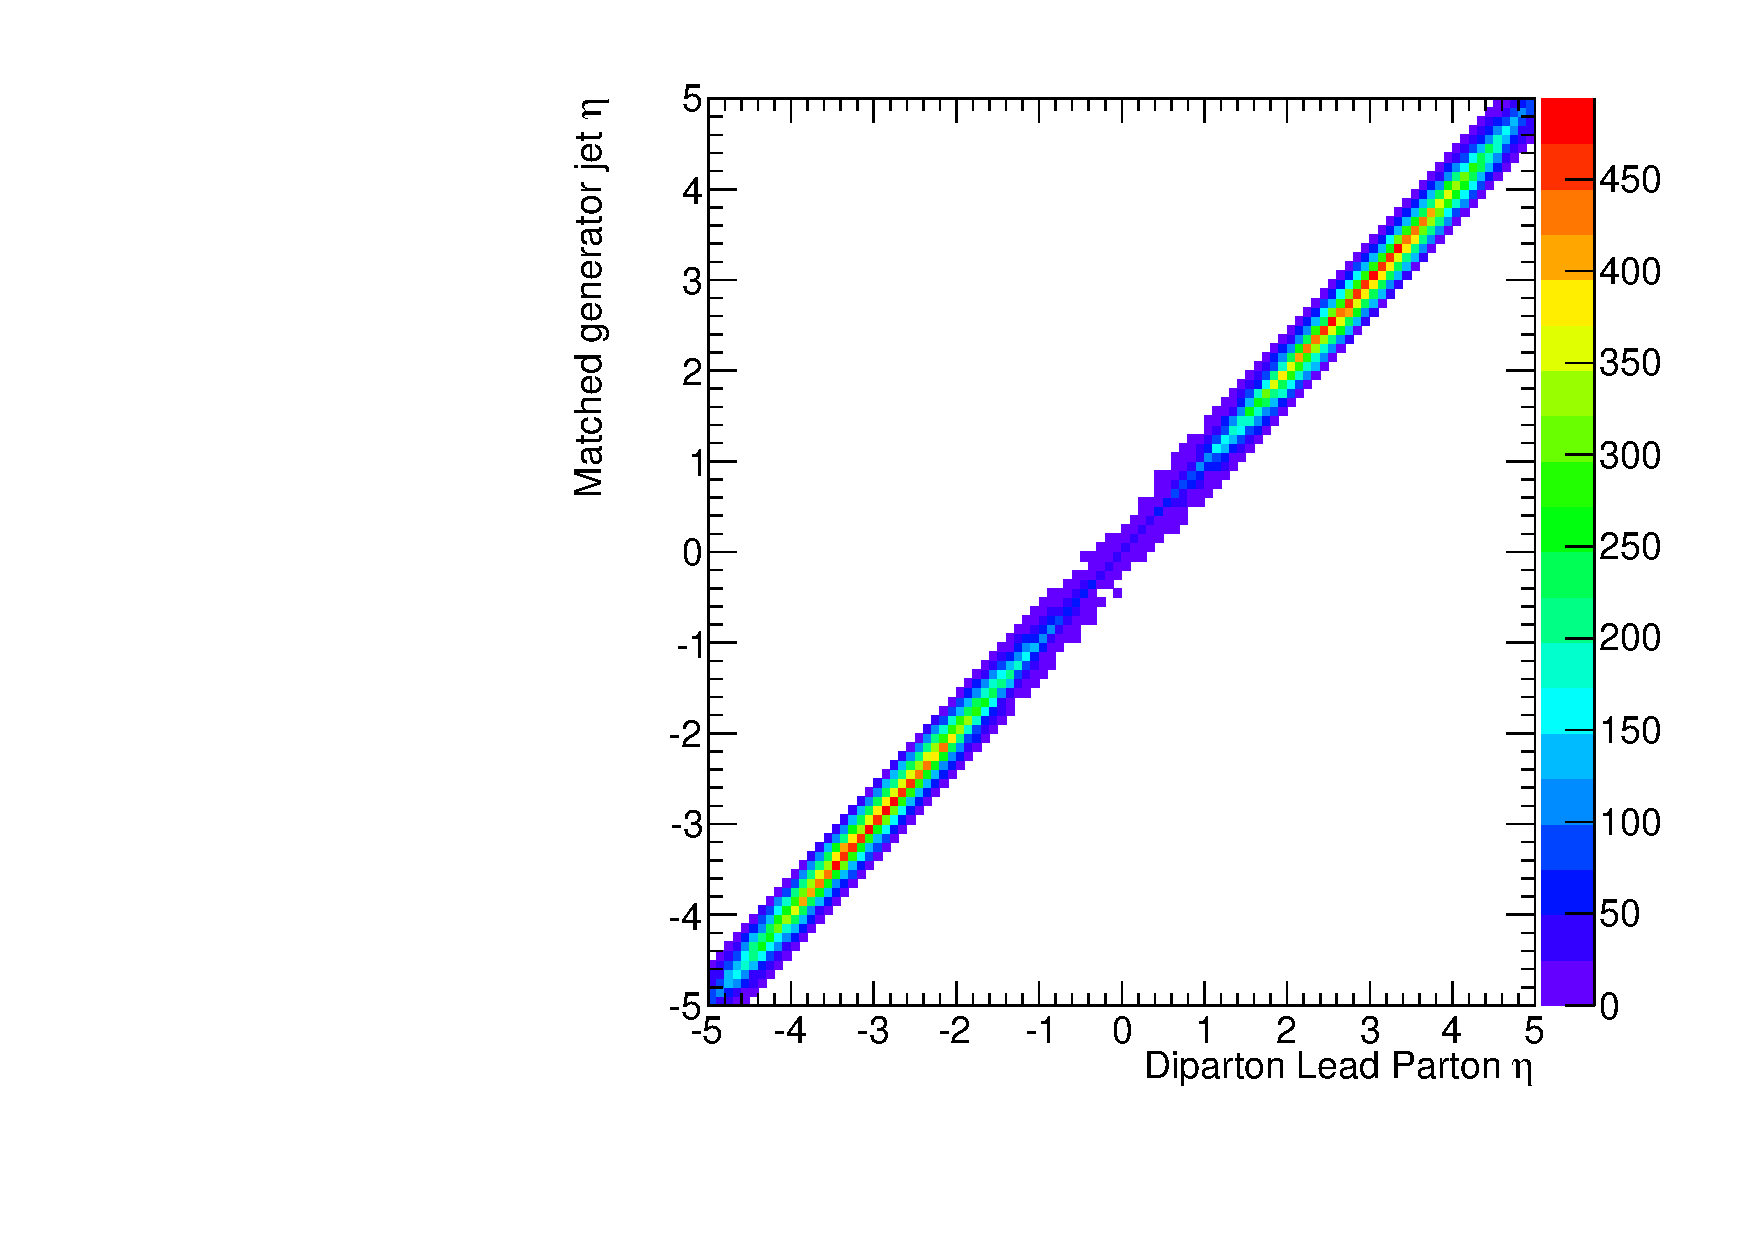
\includegraphics[width=0.40\linewidth]{Chapter08/QCDVBFSamples/Migrations/Images/SelDiParton_MatchedGenJet_Parton1_Eta.pdf}}\qquad
\subfloat[][]{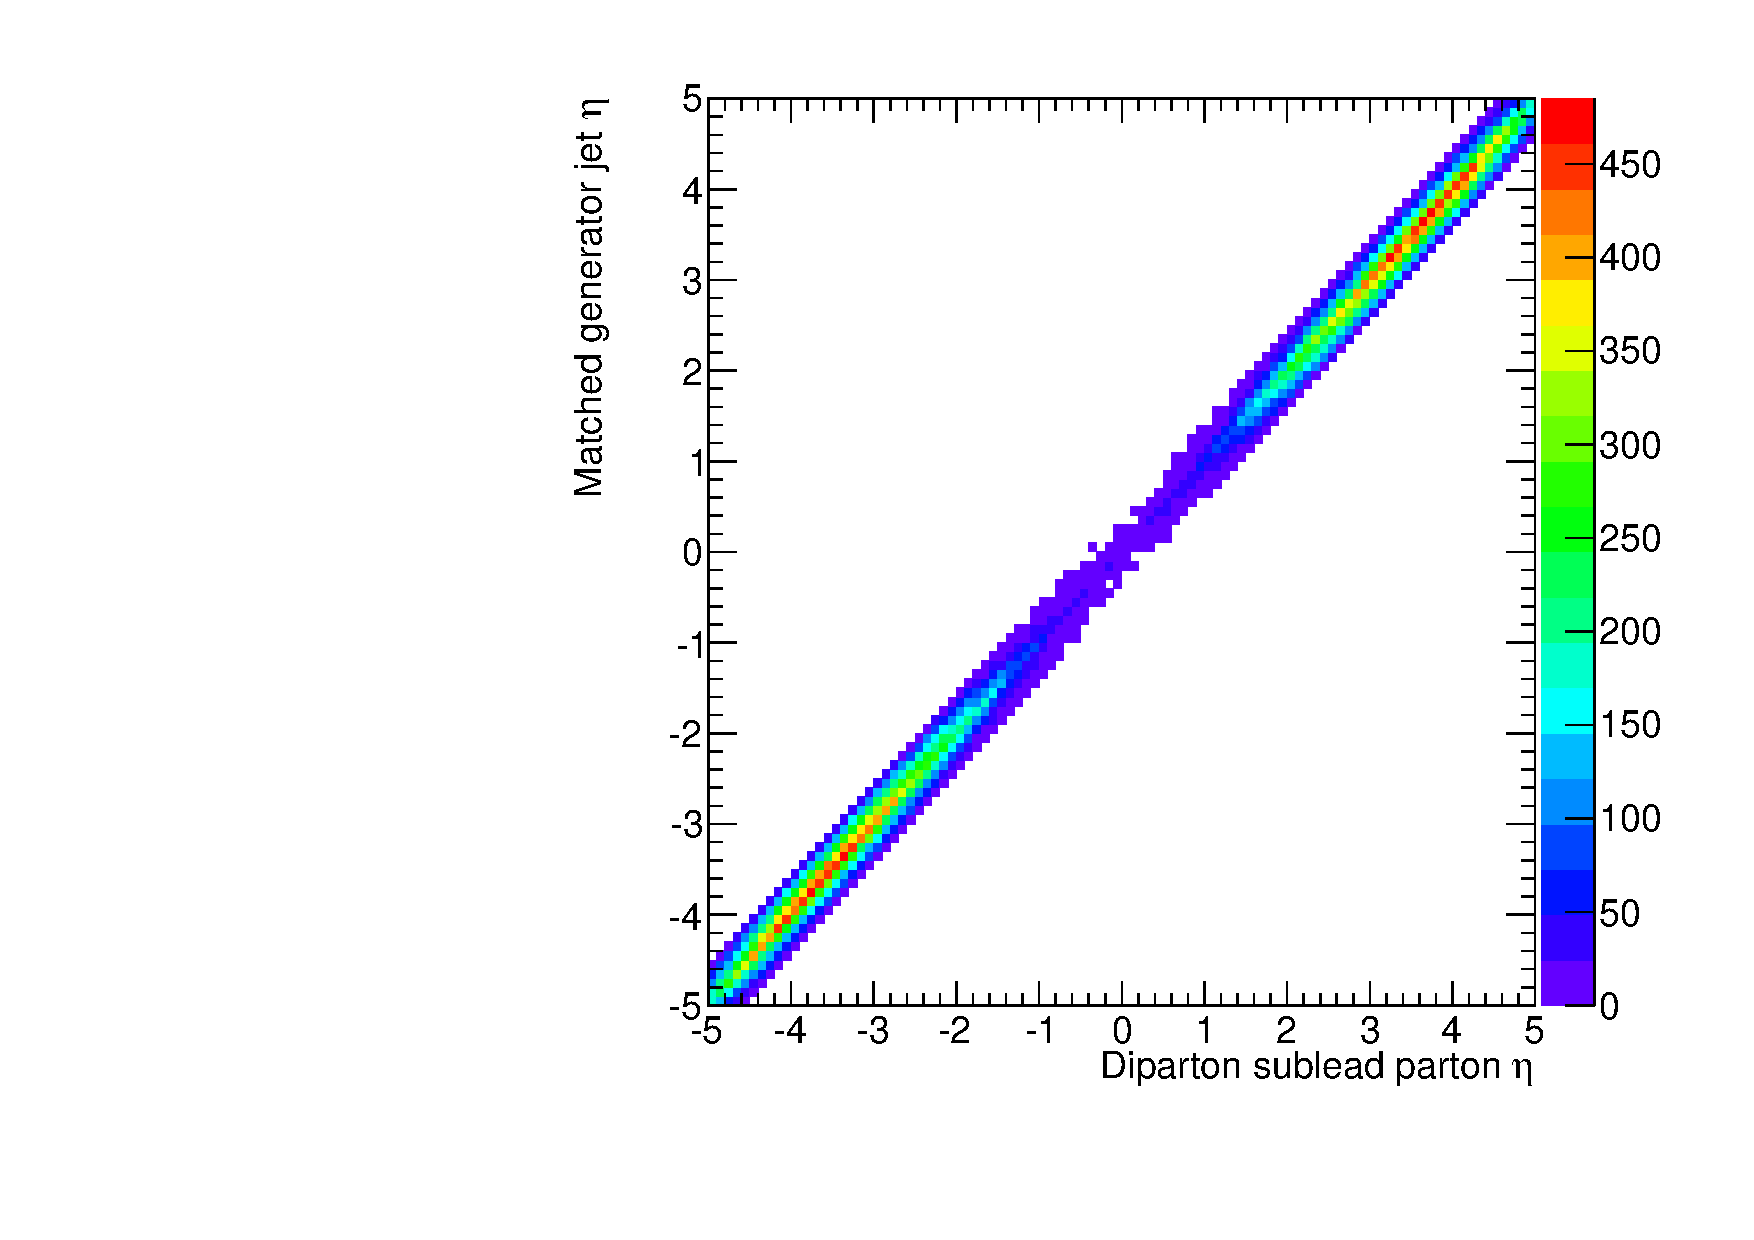
\includegraphics[width=0.40\linewidth]{Chapter08/QCDVBFSamples/Migrations/Images/SelDiParton_MatchedGenJet_Parton2_Eta.pdf}}\\
\subfloat[][]{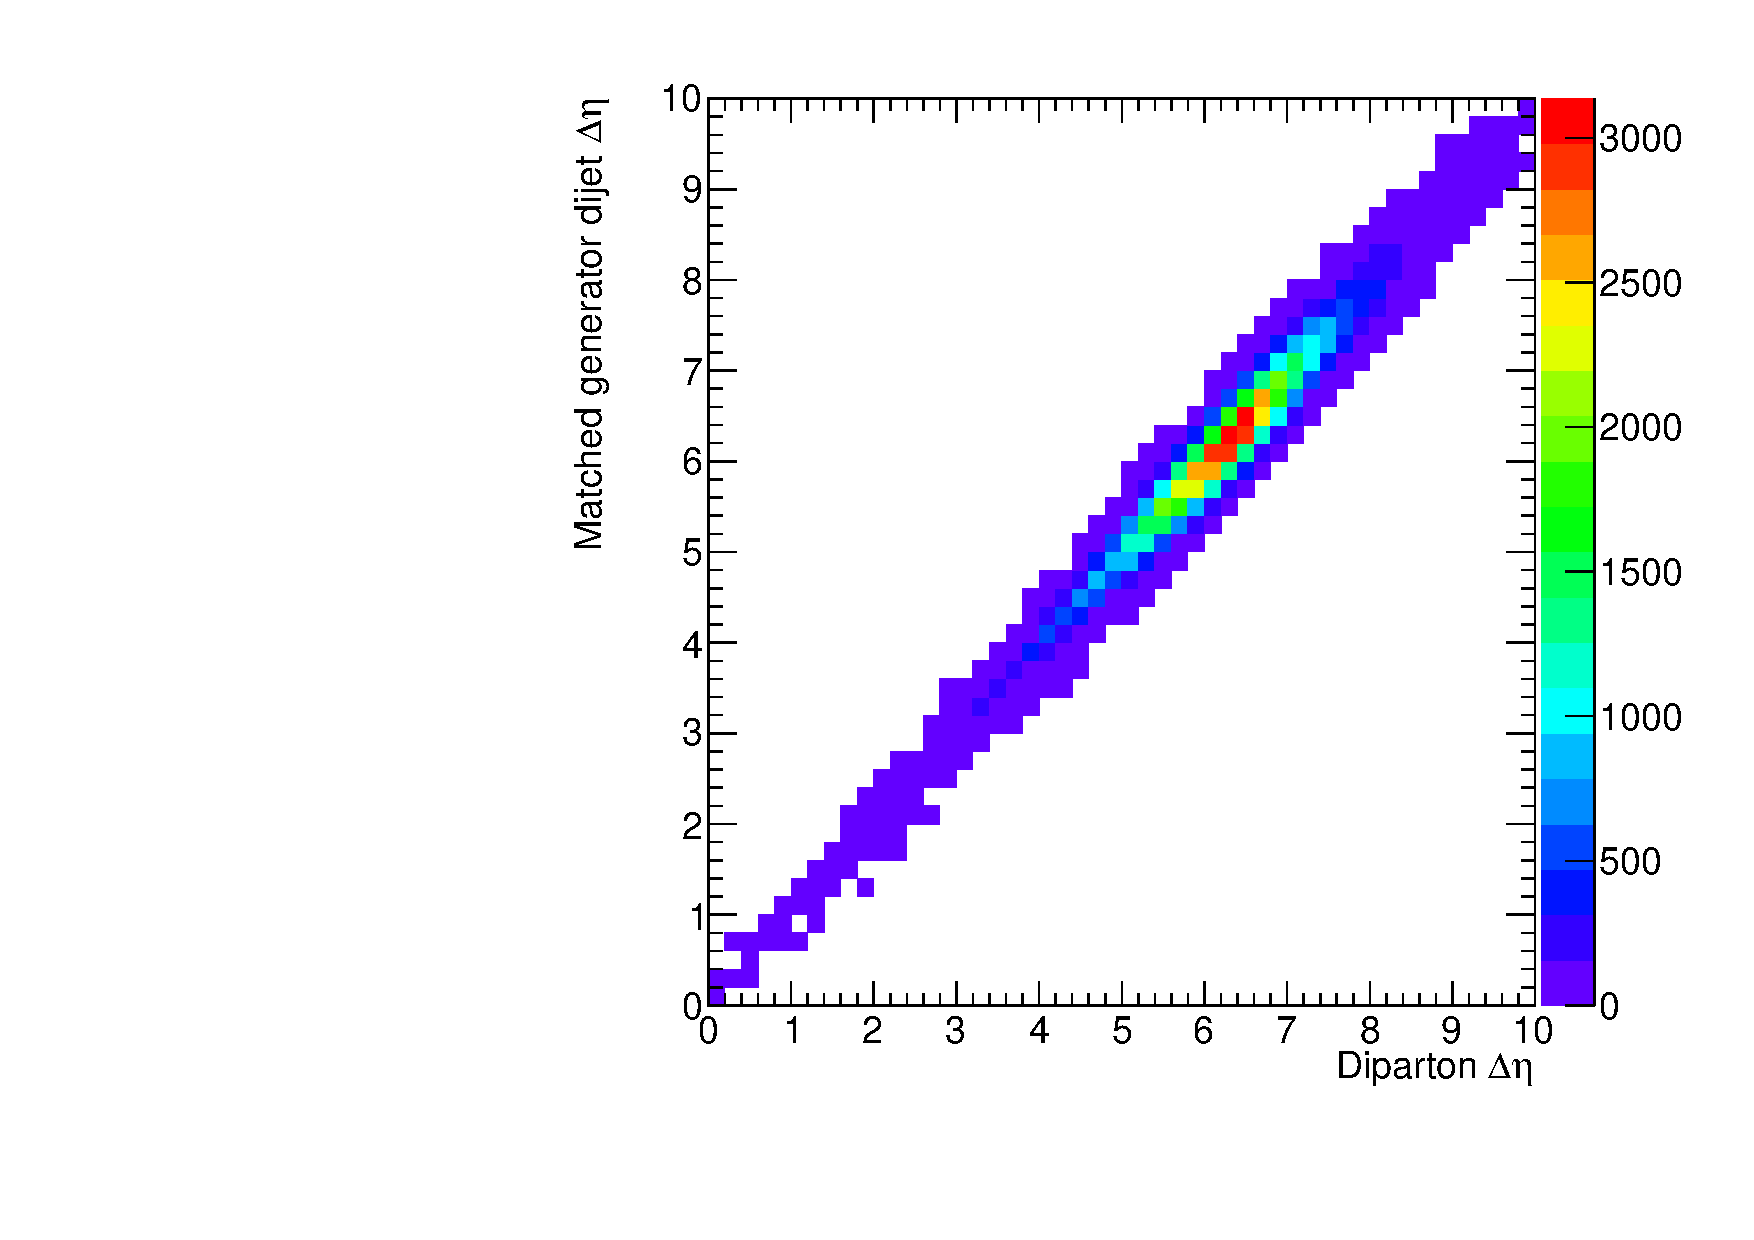
\includegraphics[width=0.40\linewidth]{Chapter08/QCDVBFSamples/Migrations/Images/SelDiParton_MatchedGenJet_DEta.pdf}}\qquad
\subfloat[][]{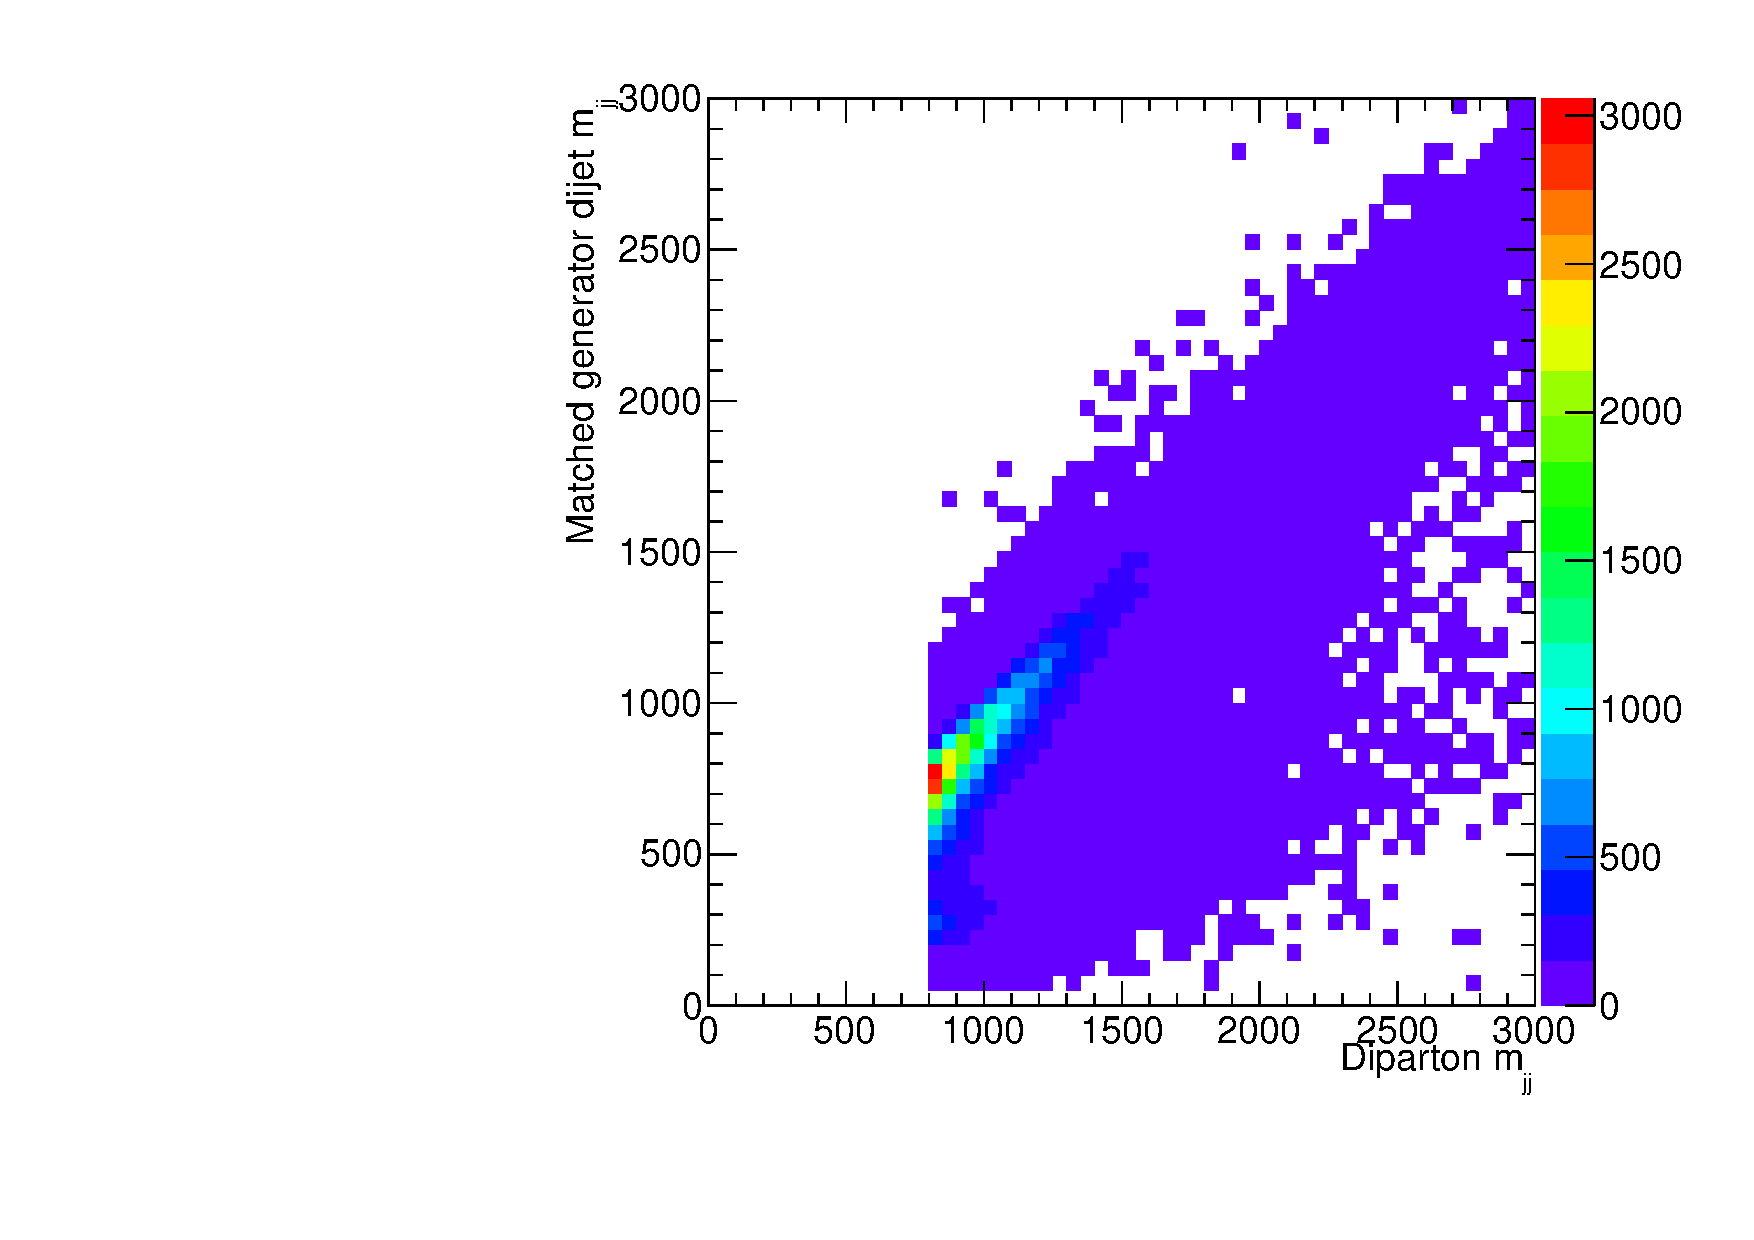
\includegraphics[width=0.40\linewidth]{Chapter08/QCDVBFSamples/Migrations/Images/SelDiParton_MatchedGenJet_Mjj.pdf}}\\
\caption[]{Plots for relevant variables of the selected di-parton against its matched dijet. On plot a) lead parton \pt b) sub-leading parton \pt c) lead parton $\eta$ d) sub-lead parton $\eta$ e) di-parton $\Delta\eta$ d) di-parton $M_{jj}$}
\label{FIGURE:RunIIPreparation_VariablesPartonVsGenJet}
\end{figure}

On plots \ref{FIGURE:RunIIPreparation_VariablesPartonVsGenJet} a), b) and f) two populations can be seen. In the parton \pt plots they are along the diagonal and along the line of generator jet \pt equal to zero and in the $M_{jj}$ plot along the diagonal and along the line of $y=x/2$. In both cases the non-diagonal population probably arises from mismatching a parton to a low \pt jet. In the $M_{jj}$ plot, the second diagonal line is due to the fact that at parton level the partons are perfectly matched in energy and momentum but if they are matched to only one correct generator jet and the other jet has \pt close to zero, the system will have half the mass of the correctly assigned events.

Event migrations can now be calculate from the events that did not pass the parton event selection but could have passed the generator level selection. This effect can be from jet dispersion, overlap, or clustering artefacts. Let's first consider the migrations on each variable separately, lead jet \pt (eq. \ref{EQUATION:RunIIPreparation_SigleVariableMigrationLeadPt}), sub-lead jet \pt (eq. \ref{EQUATION:RunIIPreparation_SigleVariableMigrationSubleadPt}) and dijet $M_{jj}$ (eq. \ref{EQUATION:RunIIPreparation_SigleVariableMigrationMjj}).

\small
\begin{equation}
\label{EQUATION:RunIIPreparation_SigleVariableMigrationLeadPt}
\frac{p_{T}^{Parton}<30 \wedge p_{T}^{GenJet} \geq 40}{p_{T}^{GenJet} \geq 40}=0.27\% \pm 0.04\%
\end{equation}

\begin{equation}
\label{EQUATION:RunIIPreparation_SigleVariableMigrationSubleadPt}
\frac{p_{T}^{Parton}<30 \wedge p_{T}^{GenJet} \geq 40}{p_{T}^{GenJet} \geq 40}=0.56\% \pm 0.08\%
\end{equation}

\begin{equation}
\label{EQUATION:RunIIPreparation_SigleVariableMigrationMjj}
\frac{M_{jj}^{Parton}<800 \wedge M_{jj}^{GenJet} \geq 1000}{M_{jj}^{GenJet} \geq 800}=0.13\% \pm 0.04\%
\end{equation}
\normalsize

Migrations of events over all variables simultaneously can now be consider using equation \ref{EQUATION:RunIIPreparation_All}.

\small
\begin{equation}
\label{EQUATION:RunIIPreparation_All}
\frac{(p_{T}^{GenJet}>40 \wedge M_{jj}^{GenJet}>1000) \wedge (p_{T}^{Parton}<30 \vee M_{jj}^{Parton}<800)}{p_{T}^{GenJet}>40 \cup M_{jj}^{GenJet}>1000} = 0.23\% \pm 0.13\%
\end{equation}
\normalsize

Global migrations of events from below the selected parton level cuts to above the selected generator cuts are of $0.23\% \pm 0.13\%$ of the total number events passing the generator filter. This is an acceptable value which should not bias in any relevant way the physics usage of this sample.

%%%%%%%%%%%%%%%%%%%%%%%%%%%%%%%%%%%%%%%%%%%%%%%%%%%%%%%%%%%%%%%%%%%%%%%%%%%%%%%%%%%%%%%
%%% SUBSECTION
%%%%%%%%%%%%%%%%%%%%%%%%%%%%%%%%%%%%%%%%%%%%%%%%%%%%%%%%%%%%%%%%%%%%%%%%%%%%%%%%%%%%%%%
\subsection{Summary}
\label{SUBSECTION:RunIIPreparation_Summary}

%Status: DONE (reviewed J.Pela x1)

The production of a new \gls{QCD} \gls{MC} event sample with \gls{VBF} characteristics was studied and all objectives were achieved. The \textsc{MADGRAPH} event generator is used and configured to produce proton-proton to two, three or four outgoing partons, where these partons can be gluons or quarks except the top quark. At this stage events are filtered by only accepting those that have at least one di-parton with $M_{jj}>800\,\GeV$ where each parton has at least $30\,\GeV$ and is contained inside the detector acceptance of $|\eta|<5.0$. This process has a cross section of $1.029 \times 10^7 \pm 1.614 \times 10^4 \,\pico\barn$. 

Event hadronization is performed using \textsc{PYTHIA 8} event generator with the MLM jet matching scheme as traditionally done in the \gls{CMS} experiment. The estimated efficiency of this step is $9.45\% \pm 0.03\%$ which leads cross section of $(9.718 \pm 0.029) \times 10^5\,\pico\barn$. From those events, the ones containing at least one generator dijet passing $\Delta\eta > 3.0$, $M_{jj} > 1000\,\GeV$, where both jets pass $\pt > 40\,\GeV$ and $|\eta|<4.8$, are kept. The sample is split into 2 sub-samples according if the dijet passing all cuts is below (sub-sample A) of above $\Delta\phi=2.15$ (sub-sample B). The filter efficiency for sub-sample A is $(2.938 \pm 0.005) \times 10^{-1}$ and this sub-sample is aimed to have $1\,\femto\barn^{-1}$ of equivalent integrated luminosity. Sub-sample B filter efficiency is $(1.125 \pm 0.009) \times 10^{-1}$ and will have $0.1-1.0\,\femto\barn^{-1}$ of equivalent integrated luminosity depending on available resources. The overlap between the two sub-samples has been estimated to be $3.95\% \pm 0.14\%$ thus requiring care in combining them.

Migrations from events below the parton level cuts to above the generator level cuts have been determined to be $0.23\% \pm 0.13\%$ of the total number of events passing the generator filters.

The \textsc{MADGRAPH} code for event generation has been approved by the \gls{CMS} \gls{MC} production team. The additional code necessary for the generator level filtering has been also approved and is queued for integration in the experiment's software. Final approval of this sample production is under way. 

%TODO: Update if sample is approved.
